%!TEX program = lualatex
%!TEX encoding = UTF-8 Unicode  
%!TEX root = chapter01.tex  
\documentclass[main.tex]{subfiles} 
\begin{document} 
%----------------------------------------------------------------------------------------
%	CHAPTER 1
%----------------------------------------------------------------------------------------
\cleardoublepage 
\loadgeometry{marginlayout}  
\pagestyle{scrheadings} % Print headers again  
\KOMAoptions{
headwidth=textwithmarginpar,
headsepline=true,
headsepline= 0.5pt,
footwidth=textwithmarginpar,
}   
\onehalfspacing 
\chapter{Fonctions quadratiques}

\begin{definition} Un monôme en $x$ de \textbf{degré $n(\in\mathbb{N})$} est une expression de la forme $ax^n$. 
Deux monômes sont semblables s'ils ont le même degré.\\
Une somme de monômes est \textbf{ordonnée réduite} si les monômes sont rangés par degré décroissant et ne sont pas semblables.  
\end{definition}
\begin{example} 
	\begin{enumerate}[leftmargin=*, label=\textbullet]
		\item   $5$, $0$ sont des termes constants.  
	\item   $4x^3$ est un monôme de degré $3$. Le coefficient est $4$.
	\item   $-x$ est un monôme de degré $1$. Le coefficient est $-1$.
\end{enumerate} 
\end{example}
\begin{example}  $3x+5$ est un polynôme ordonné réduit de degré 1.\sidenote{expression \textbf{affine} en $x$}  
\begin{enumerate}[leftmargin=*, label=\textbullet]
%	\item $3x+5$ est un polynôme ordonné réduit de degré 1.\sidenote{expression \textbf{affine} en $x$}
	\item $-3x^2+2x+5$ est un polynôme ordonné réduit de degré 2.\sidenote{expression \textbf{quadratique} en $x$}
	\item $5x^3-x^2+5$ est un polynôme ordonné réduit de degré 3.\sidenote{expression \textbf{cubique} en $x$}
\end{enumerate} 
\end{example} 
\begin{definition} Une fonction	définie sur $\mathbb{R}$ 
%	$f\colon \begin{aligned}[t] \mathbb{R}&\to \mathbb{R}\\
%		x&\mapsto y=f(x)\end{aligned}$ 
est une fonction polynôme de degré 2\sidenote{nous dirons fonction quadratique} 
	si il existe $a\neq0$, $b$ et $c\in\mathbb{R}$ tel que : 
	\setlength{\abovedisplayskip}{3pt}
	\setlength{\belowdisplayskip}{3pt}
	$$\text{pour tout} \;x\in\mathbb{R} \qquad f(x)=ax^2+bx+c$$   
Sa représentation graphique s'appelle une \textbf{parabole}.
\end{definition} 
\begin{figure*}[!h] 
	\begin{tikzpicture}[xscale=0.9, yscale=0.9,
		xkcd/.style={
			decoration={
				name=random steps,
				segment length=2pt,
				amplitude=0.3pt,
			},
			line width=1pt,
			line join=round,
			line cap=round,
			decorate,
			>=Classical TikZ Rightarrow ,   
		},   
		] 
		\tkzSetUpPoint[size=3, fill=black]
		\tkzfctset{tan style/.style={->,>=latex, color=red, line width=1.2pt}}  
		\tkzInit[xmin=-4,xmax=4,ymin=-1,ymax=6.5,xstep=1.0, ystep=1.0]; 
		\tkzDrawX[  xkcd ,>=Classical TikZ Rightarrow,  font=\scriptsize, line width=2pt, label={\fontspec{xkcd Script}x}   ] 
		\tkzDrawY[  xkcd ,>=Classical TikZ Rightarrow, noticks,  font=\scriptsize, line width=2pt , label={\fontspec{xkcd Script}y}  ]  
		%	\tkzLabelX[xkcd ,   font= \scriptsize  ]
		\foreach \i in {-4,-3,...,4}{  
			\tkzText[below=1pt, font=\scriptsize,fill=white](\i,0){\fontspec{xkcd}{\i}}
		}
		
		
		\def\a{0.25}
		\def\b{0.75}
		\def\c{1.5}
		
		
		\tkzFct[xkcd, domain = -4.0:4.0, line width=1.2pt, samples=25, color = blue]{\a*x**2+\b*x+\c}   
		\tkzFct[xkcd, domain = -4.0:4.0, line width=1.2pt, samples=2, color = blue, dashed]{\b*x+\c} 
		
		\tkzFct[xkcd, domain = 2.35:3.65, line width=1.2pt, samples=2, color = blue]{\b*\x+\c-1}  
		\foreach \i in {-3,-2,-1,1,2,3}{  
			\pgfmathparse{\i*\i} \let \ii \pgfmathresult;
			\tkzDefPointByFct[with=a](\i) \tkzGetPoint{A}% \tkzDrawPoint[color = blue](A) 
			\tkzDefPointByFct[with=b](\i) \tkzGetPoint{B}% \tkzDrawPoint[color = blue](B)  
			\tkzDrawSegments[xkcd ,->,line width=1pt,  color=blue,dashed](B,A) 
			\tkzLabelSegment[right,font=\scriptsize](B,A){\fontspec{xkcd Script}\pgfmathprintnumber{\ii}a} 
		}  
		
		\tkzDefPointByFct[with=c](2.5) \tkzGetPoint{P}
		\tkzDefPointByFct[with=c](3.5) \tkzGetPoint{Q} 
		\tkzGetPointCoord(P){P}
		\tkzGetPointCoord(Q){Q}
		\tkzDefPoint(\Qx,\Py){R} 
		\tkzDrawSegments[xkcd, line width=1pt, color=blue,dashed](P,R R,Q) 
		\tkzLabelSegment[right,font=\small](R,Q){\fontspec{xkcd Script}b}
		\tkzLabelSegment[below,font=\small](P,R){\fontspec{xkcd Script}1} 
		
		\tkzText[below right, font=\small](0,\c){\fontspec{xkcd Script}c}
		\tkzText[draw,xkcd, font=\small](-3,6){\fontspec{xkcd Script}f(x)=ax$^2$+bx+c}
		\tkzText[draw,xkcd, font=\small](-3,5){\fontspec{xkcd Script}a>0}
		
	\end{tikzpicture} 
	\begin{tikzpicture}[xscale=0.9, yscale=0.9,
		xkcd/.style={
			decoration={
				name=random steps,
				segment length=2pt,
				amplitude=0.3pt,
			},
			line width=1pt,
			line join=round,
			line cap=round,
			decorate,
			>=Classical TikZ Rightarrow ,  
		},     
		] 
		
		
		
		\tkzSetUpPoint[size=3, fill=black]
		\tkzfctset{tan style/.style={->,>=latex, color=red, line width=1.2pt}}  
		\tkzInit[xmin=-4,xmax=4,ymin=-3,ymax=4.5,xstep=1.0, ystep=1.0]; 
		\tkzDrawX[  xkcd ,>=Classical TikZ Rightarrow,   font=\scriptsize, line width=2pt, label={\fontspec{xkcd Script}x}   ] 
		\tkzDrawY[  xkcd ,>=Classical TikZ Rightarrow, noticks,  font=\scriptsize, line width=2pt , label={\fontspec{xkcd Script}y}  ]  
		%	\tkzLabelX[xkcd ,   font= \scriptsize  ]
		\foreach \i in {-4,-3,...,4}{  
			\tkzText[below=1pt, font=\scriptsize,fill=white](\i,0){\fontspec{xkcd}{\i}}
		}
		
		\def\a{(-0.25)}
		\def\b{(0.75)}
		\def\c{(1.75)}
		
		
		\tkzFct[xkcd, domain = -4.0:4.0, line width=1.2pt, samples=25, color = blue]{\a*x**2+\b*x+\c+0.0}   
		\tkzFct[xkcd, domain = -4.0:4.0, line width=1.2pt, samples=2, color = blue, dashed]{\b*x+\c} 
		
		\tkzFct[xkcd, domain = -3.65:-2.35, line width=1.2pt, samples=2, color = blue]{\b*\x+\c+2}  
		
		\foreach \i in {-3.0,-2.0,-1.0,1.0,2.0,3.0}{  
			\pgfmathparse{\i*\i} \let \ii \pgfmathresult;
			\tkzDefPointByFct[with=a](\i) \tkzGetPoint{A}  
			\tkzDefPointByFct[with=b](\i) \tkzGetPoint{B}  
			\tkzDrawSegments[xkcd ,->,line width=1pt,  color=blue,dashed](B,A) 
			\tkzLabelSegment[right,font=\scriptsize](B,A){\fontspec{xkcd Script}\pgfmathprintnumber{\ii}a} 
		}  
		
		\tkzDefPointByFct[with=c](-3.5) \tkzGetPoint{P}
		\tkzDefPointByFct[with=c](-2.5) \tkzGetPoint{Q} 
		\tkzGetPointCoord(P){P}
		\tkzGetPointCoord(Q){Q}
		\tkzDefPoint(\Qx,\Py){R} 
		\tkzDrawSegments[xkcd, line width=1pt, color=blue,dashed](P,R R,Q) 
		\tkzLabelSegment[right,font=\small](R,Q){\fontspec{xkcd Script}b}
		\tkzLabelSegment[below,font=\small](P,R){\fontspec{xkcd Script}1} 
		
		\tkzText[below right, font=\small](0,\c){\fontspec{xkcd Script}c}
%			\tkzText[draw,xkcd, font=\small](-3,3.5){\fontspec{xkcd Script}f(x)=ax$^2$+bx+c}
					\tkzText[draw,xkcd, font=\small](-3,3.0){\fontspec{xkcd Script}a<0}
	\end{tikzpicture}
%\caption{Représentation graphique d'une fonction quadratique $f(x)=ax^2+bx+c$, cas $a>0$ et $a<0$.}
\end{figure*}

%----------------------------------------------------------------------------------------
%	EXERCICES
%----------------------------------------------------------------------------------------

\newpage 
\loadgeometry{widelayout}  
\pagestyle{scrheadings} % Print headers again  
\KOMAoptions{
	headwidth=textwithmarginpar,
	headsepline=true,
	headsepline= 0.5pt,
	footwidth=textwithmarginpar,
} 
\onehalfspacing
\begin{example} Représentez les courbes $\mathscr{P}$ données par leur équation.
	
	\end{example}  
\noindent  \hfill
$\mathscr{P}_1\colon y=2x^2$
\hfill 
$\mathscr{P}_2\colon y=-x^2$
\hfill \null

\noindent 
\parbox{0.15\linewidth}{
	\begin{tabularx}{1\linewidth}{?c?Y?}\hline
		$  x $& $y$ \\ \hline
		$-3$&  \\ \hline
		$-2$&  \\ \hline
		$-1$&  \\ \hline
		$0$&  \\ \hline
		$1$&  \\ \hline
		$2$&  \\ \hline
		$3$ &  \\ \hline
	\end{tabularx}
}
\parbox{0.32\linewidth}{ 
	\begin{tikzpicture}[xscale=0.75, yscale=1.2]
		%----------------------- 
		\tkzSetUpPoint[size=3, fill=black]
		\tkzfctset{tan style/.style={->,>=latex, color=red, line width=1.2pt}}  
		\tkzInit[xmin=-3,xmax=3,ymin=-5,ymax=20,xstep=1.0, ystep=5.0  ];
		\tkzGrid[color=gray, line width=0.5pt,]
		\begin{scope}[dashed] 
			\tkzGrid[sub,subxstep=1, subystep=1,color=gray, line width=0.5pt, ]
		\end{scope}  
		\tkzDrawX[  noticks, font=\scriptsize, line width=2pt, label=$x$, above =5pt  ] 
		\tkzDrawY[  noticks,  font=\scriptsize, line width=2pt , up space=0.2pt, label={$y$}, right=5pt, ]  
		\tkzLabelXY[orig = false,  font=\scriptsize]
		%	\tkzRep[color  = Maroon,line width = 2pt, posxlabel=below, posylabel=left, xnorm=1, ynorm=1]
		%----------------------- 
%		\tkzFct[domain = -3.0:6.0, line width=2pt,samples=100,color = blue]{(2*\x**2)}   
		%-----------------------  
	\end{tikzpicture} 
}
\parbox{0.15\linewidth}{
	\begin{tabularx}{1\linewidth}{?c?Y?}\hline
		$  x $& $y$ \\ \hline
		$-3$&  \\ \hline
		$-2$&  \\ \hline
		$-1$&  \\ \hline
		$0$&  \\ \hline
		$1$&  \\ \hline
		$2$&  \\ \hline
		$3$ &  \\ \hline
	\end{tabularx}
}
\parbox{0.32\linewidth}{ 
	\begin{tikzpicture}[xscale=0.75, yscale=0.9]
		%----------------------- 
		\tkzSetUpPoint[size=3, fill=black]
		\tkzfctset{tan style/.style={->,>=latex, color=red, line width=1.2pt}}  
		\tkzInit[xmin=-4,xmax=4,ymin=-10,ymax=2,xstep=1.0, ystep=2.0  ];
		\tkzGrid[color=gray, line width=0.5pt,]
		\begin{scope}[dashed] 
			\tkzGrid[sub,subxstep=1, subystep=1,color=gray, line width=0.5pt, ]
		\end{scope}  
		\tkzDrawX[  noticks, font=\scriptsize, line width=2pt, label=$x$, above =5pt  ] 
		\tkzDrawY[  noticks,  font=\scriptsize, line width=2pt , up space=0.2pt, label={$y$}, right=5pt, ]  
		\tkzLabelXY[orig = false,  font=\scriptsize]
		%	\tkzRep[color  = Maroon,line width = 2pt, posxlabel=below, posylabel=left, xnorm=1, ynorm=1]
		%----------------------- 
%		\tkzFct[domain = -4.0:6.0, line width=2pt,samples=100,color = blue]{(-1*\x**2)}   
		%-----------------------  
	\end{tikzpicture} 
}


\noindent \hfill
$\mathscr{P}_3\colon y=x^2-3$
\hfill 
$\mathscr{P}_4\colon y=(x-2)^2$
\hfill \null

\noindent 
\parbox{0.15\linewidth}{
\begin{tabularx}{1\linewidth}{?c?Y?}\hline
	$  x $& $y$ \\ \hline
	$-3$&  \\ \hline
	$-2$& $1$ \\ \hline
	$-1$&  \\ \hline
	$0$&  \\ \hline
	$1$&  \\ \hline
	$2$&  \\ \hline
	$3$ &  \\ \hline
\end{tabularx}
}
\parbox{0.32\linewidth}{ 
\begin{tikzpicture}[xscale=0.8, yscale=2.1]
	%----------------------- 
	\tkzSetUpPoint[size=3, fill=black]
	\tkzfctset{tan style/.style={->,>=latex, color=red, line width=1.2pt}}  
	\tkzInit[xmin=-3,xmax=3,ymin=-5,ymax=10,xstep=1.0, ystep=5.0  ];
		\tkzGrid[color=gray, line width=0.5pt,]
	\begin{scope}[dashed] 
		\tkzGrid[sub,subxstep=1, subystep=1,color=gray, line width=0.5pt, ]
	\end{scope}  
	\tkzDrawX[  noticks, font=\scriptsize, line width=2pt, label=$x$, above =5pt  ] 
	\tkzDrawY[  noticks,  font=\scriptsize, line width=2pt , up space=0.2pt, label={$y$}, right=5pt, ]  
	\tkzLabelXY[orig = false,  font=\scriptsize]
%	\tkzRep[color  = Maroon,line width = 2pt, posxlabel=below, posylabel=left, xnorm=1, ynorm=1]
	%----------------------- 
%	\tkzFct[domain = -3.0:6.0, line width=2pt,samples=100,color = blue]{(\x**2-3)}   
	%----------------------- 
%	\tkzDefPointByFct(3) \tkzGetPoint{A}
%	\tkzDefPointByFct(6) \tkzGetPoint{B}
%	\tkzDefPointByFct(4.5) \tkzGetPoint{D}
%	\tkzGetPointCoord(A){A}
%	\tkzGetPointCoord(B){B}
%	\tkzDefPoint(\Bx,\Ay){C}
%	\tkzDrawSegments[line width=1pt, color=blue,dashed](A,C C,B) 
%	\tkzLabelSegment[right,font=\scriptsize](C,B){$2$}
%	\tkzLabelSegment[below,font=\scriptsize](A,C){$3$}
%	\tkzText[above left,color=blue,font=\scriptsize](D){$m=\frac{2}{3}$}
%	\tkzText[below, draw, font=\scriptsize,fill=white](4,-1){$f(x)=\frac{2}{3}x+1$}  
	%	\tkzPointShowCoord[ color=blue, line width=1.2pt  ](1,1) \tkzPointShowCoord[  color=blue, line width=1.2pt ](-1,1) 
\end{tikzpicture} 
}
\parbox{0.15\linewidth}{
\begin{tabularx}{1\linewidth}{?c?Y?}\hline
	$  x $& $y$ \\ \hline 
	$-2$& -4  \\ \hline
	$-1$&  \\ \hline
	$0$&  \\ \hline
	$1$&  \\ \hline
	$2$&  \\ \hline
	$3$ & -9 \\ \hline 
\end{tabularx}
}
\parbox{0.32\linewidth}{ 
\begin{tikzpicture}[xscale=0.75, yscale=0.75]
	%----------------------- 
	\tkzSetUpPoint[size=3, fill=black]
	\tkzfctset{tan style/.style={->,>=latex, color=red, line width=1.2pt}}  
	\tkzInit[xmin=-3,xmax=5,ymin=-2,ymax=16,xstep=1.0, ystep=2.0  ];
	\tkzGrid[color=gray, line width=0.5pt,]
	\begin{scope}[dashed] 
		\tkzGrid[sub,subxstep=1, subystep=1,color=gray, line width=0.5pt, ]
	\end{scope}  
	\tkzDrawX[  noticks, font=\scriptsize, line width=2pt, label=$x$, above =5pt  ] 
	\tkzDrawY[  noticks,  font=\scriptsize, line width=2pt , up space=0.2pt, label={$y$}, right=5pt, ]  
	\tkzLabelXY[orig = false,  font=\scriptsize]
	%	\tkzRep[color  = Maroon,line width = 2pt, posxlabel=below, posylabel=left, xnorm=1, ynorm=1]
	%----------------------- 
%	\tkzFct[domain = -3.0:5.0, line width=2pt,samples=100,color = blue]{((\x-2)**2)}   
	%-----------------------  
\end{tikzpicture} 
}



\noindent  \hfill
$\mathscr{P}_5\colon y=x^2+3$
\hfill 
$\mathscr{P}_6\colon y=(x+1)^2$
\hfill \null

\noindent
\parbox{0.15\linewidth}{
	\begin{tabularx}{1\linewidth}{?c?Y?}\hline
		$  x $& $y$ \\ \hline  
		$-3$ &  \\ \hline
		$-2$&  $7$\\ \hline
		$-1$&  \\ \hline
		$0$&  \\ \hline
		$1$&  \\ \hline
		$2$&  \\ \hline
		$3$ &  \\ \hline
	\end{tabularx}
}
\parbox{0.39\linewidth}{ 
	\begin{tikzpicture}[xscale=1, yscale=1.00]
		%----------------------- 
		\tkzSetUpPoint[size=3, fill=black]
		\tkzfctset{tan style/.style={->,>=latex, color=red, line width=1.2pt}}  
		\tkzInit[xmin=-3,xmax=3,ymin=-2,ymax=12,xstep=1.0, ystep=2.0  ];
		\tkzGrid[color=gray, line width=0.5pt,]
		\begin{scope}[dashed] 
			\tkzGrid[sub,subxstep=1, subystep=1,color=gray, line width=0.5pt, ]
		\end{scope}  
		\tkzDrawX[  noticks, font=\scriptsize, line width=2pt, label=$x$, above =5pt  ] 
		\tkzDrawY[  noticks,  font=\scriptsize, line width=2pt , up space=0.2pt, label={$y$}, right=5pt, ]  
		\tkzLabelXY[orig = false,  font=\scriptsize]
		%	\tkzRep[color  = Maroon,line width = 2pt, posxlabel=below, posylabel=left, xnorm=1, ynorm=1]
		%----------------------- 
%		\tkzFct[domain = -3.0:5.0, line width=2pt,samples=100,color = blue]{((\x)**2+3)}   
		%-----------------------  
	\end{tikzpicture} 
}
\parbox{0.15\linewidth}{
	\begin{tabularx}{1\linewidth}{?c?Y?}\hline
		$  x $& $y$ \\ \hline  
		$-3$ &  \\ \hline
		$-2$&  \\ \hline
		$-1$&  \\ \hline
		$0$&  \\ \hline
		$1$&  \\ \hline
		$2$&  \\ \hline
		$3$ &  \\ \hline
	\end{tabularx}
}
\parbox{0.30\linewidth}{ 
\begin{tikzpicture}[xscale=0.75, yscale=1.15]
	%----------------------- 
	\tkzSetUpPoint[size=3, fill=black]
	\tkzfctset{tan style/.style={->,>=latex, color=red, line width=1.2pt}}  
	\tkzInit[xmin=-4,xmax=3,ymin=-2,ymax=10,xstep=1.0, ystep=2.0  ];
	\tkzGrid[color=gray, line width=0.5pt,]
	\begin{scope}[dashed] 
		\tkzGrid[sub,subxstep=1, subystep=1,color=gray, line width=0.5pt, ]
	\end{scope}  
	\tkzDrawX[  noticks, font=\scriptsize, line width=2pt, label=$x$, above =5pt  ] 
	\tkzDrawY[  noticks,  font=\scriptsize, line width=2pt , up space=0.2pt, label={$y$}, right=5pt, ]  
	\tkzLabelXY[orig = false,  font=\scriptsize]
	%	\tkzRep[color  = Maroon,line width = 2pt, posxlabel=below, posylabel=left, xnorm=1, ynorm=1]
	%----------------------- 
%	\tkzFct[domain = -4.0:5.0, line width=2pt,samples=100,color = blue]{((\x+1)**2)}   
	%-----------------------  
\end{tikzpicture} 
}

\newpage
\begin{example} Dans chaque cas, représentez la courbe $\mathscr{P}$ et la droite $d$.
\end{example}   
\noindent  \hfill
$\mathscr{P}_1\colon y=x^2-x+3$ et $d\colon  y = -x+3$
\hfill 
$\mathscr{P}_2\colon y=x^2 +x-3$ et $d\colon y= x-3$
\hfill \null

\noindent 
\parbox{0.15\linewidth}{
	\begin{tabularx}{1\linewidth}{?c?Y?}\hline
		$  x $& $y$ \\ \hline
		$-3$&  \\ \hline
		$-2$&  \\ \hline
		$-1$&  \\ \hline
		$0$&  \\ \hline
		$1$&  \\ \hline
		$2$&  \\ \hline
		$3$ &  \\ \hline
	\end{tabularx}
}
\parbox{0.35\linewidth}{ 
\begin{tikzpicture}[xscale=0.75, yscale=0.8]
	%----------------------- 
	\tkzSetUpPoint[size=3, fill=black]
	\tkzfctset{tan style/.style={->,>=latex, color=red, line width=1.2pt}}  
	\tkzInit[xmin=-4,xmax=4,ymin=0,ymax=16,xstep=1.0, ystep=2.0  ];
	\tkzGrid[color=gray, line width=0.5pt,]
	\begin{scope}[dashed] 
		\tkzGrid[sub,subxstep=1, subystep=1,color=gray, line width=0.5pt, ]
	\end{scope}  
	\tkzDrawX[  noticks, font=\scriptsize, line width=2pt, label=$x$, above =5pt  ] 
	\tkzDrawY[  noticks,  font=\scriptsize, line width=2pt , up space=0.2pt, label={$y$}, right=5pt, ]  
	\tkzLabelXY[orig = false,  font=\scriptsize]
	%	\tkzRep[color  = Maroon,line width = 2pt, posxlabel=below, posylabel=left, xnorm=1, ynorm=1]
	%----------------------- 
%	\tkzFct[domain = -4.0:6.0, line width=2pt,samples=100,color = blue]{(1*\x**2-\x+3)} 
%	\tkzFct[domain = -4.0:6.0, line width=2pt,samples=100,color = red]{(-\x+3)}    
	%-----------------------  
\end{tikzpicture} 
}
\parbox{0.15\linewidth}{
	\begin{tabularx}{1\linewidth}{?c?Y?}\hline
		$  x $& $y$ \\ \hline
		$-3$&  \\ \hline
		$-2$&  \\ \hline
		$-1$&  \\ \hline
		$0$&  \\ \hline
		$1$&  \\ \hline
		$2$&  \\ \hline
		$3$ &  \\ \hline
	\end{tabularx}
}
\parbox{0.30\linewidth}{ 
	\begin{tikzpicture}[xscale=0.75, yscale=1.6]
		%----------------------- 
		\tkzSetUpPoint[size=3, fill=black]
		\tkzfctset{tan style/.style={->,>=latex, color=red, line width=1.2pt}}  
		\tkzInit[xmin=-3,xmax=3,ymin=-5,ymax=15,xstep=1.0, ystep=5.0  ];
		\tkzGrid[color=gray, line width=0.5pt,]
		\begin{scope}[dashed] 
			\tkzGrid[sub,subxstep=1, subystep=1,color=gray, line width=0.5pt, ]
		\end{scope}  
		\tkzDrawX[  noticks, font=\scriptsize, line width=2pt, label=$x$, above =5pt  ] 
		\tkzDrawY[  noticks,  font=\scriptsize, line width=2pt , up space=0.15pt, label={$y$}, right=5pt, ]  
		\tkzLabelXY[orig = false,  font=\scriptsize]
		%	\tkzRep[color  = Maroon,line width = 2pt, posxlabel=below, posylabel=left, xnorm=1, ynorm=1]
		%----------------------- 
%		\tkzFct[domain = -4.0:6.0, line width=2pt,samples=100,color = blue]{(1*\x**2+\x-3)}   
%		\tkzFct[domain = -4.0:6.0, line width=2pt,samples=100,color = red]{(\x-3)}   
		%-----------------------  
	\end{tikzpicture} 
}

\noindent  \hfill
$\mathscr{P}_3\colon y=2x^2+5x$ et $d\colon  y = 5x$
\hfill 
$\mathscr{P}_4\colon y=-x^2 +x$ et $d\colon y=  x$
\hfill \null

\noindent 
\parbox{0.15\linewidth}{
	\begin{tabularx}{1\linewidth}{?c?Y?}\hline
		$  x $& $y$ \\ \hline
		$-4$&  \\ \hline
		$-3$&  \\ \hline
		$-2$&  \\ \hline
		$-1$&  \\ \hline
		$0$&  \\ \hline
		$1$&  \\ \hline
		$2$&  \\ \hline 
	\end{tabularx}
}
\parbox{0.38\linewidth}{ 
\begin{tikzpicture}[xscale=0.70, yscale=1.2]
	%----------------------- 
	\tkzSetUpPoint[size=3, fill=black]
	\tkzfctset{tan style/.style={->,>=latex, color=red, line width=1.2pt}}  
	\tkzInit[xmin=-6,xmax=3,ymin=-5,ymax=20,xstep=1.0, ystep=5.0  ];
	\tkzGrid[color=gray, line width=0.5pt,]
	\begin{scope}[dashed] 
		\tkzGrid[sub,subxstep=1, subystep=1,color=gray, line width=0.5pt, ]
	\end{scope}  
	\tkzDrawX[  noticks, font=\scriptsize, line width=2pt, label=$x$, above =5pt  ] 
	\tkzDrawY[  noticks,  font=\scriptsize, line width=2pt , up space=0.2pt, label={$y$}, right=5pt, ]  
	\tkzLabelXY[orig = false,  font=\scriptsize]
	%	\tkzRep[color  = Maroon,line width = 2pt, posxlabel=below, posylabel=left, xnorm=1, ynorm=1]
	%----------------------- 
%	\tkzFct[domain = -5.0:6.0, line width=2pt,samples=100,color = blue]{(2*\x**2+5*\x)} 
%	\tkzFct[domain = -5.0:6.0, line width=2pt,samples=100,color = red]{(5*\x)}    
	%-----------------------  
\end{tikzpicture} 
}
\parbox{0.15\linewidth}{
\begin{tabularx}{1\linewidth}{?c?Y?}\hline
	$  x $& $y$ \\ \hline
	$-3$&  \\ \hline
	$-2$&  \\ \hline
	$-1$&  \\ \hline
	$0$&  \\ \hline
	$1$&  \\ \hline
	$2$&  \\ \hline
	$3$ &  \\ \hline
\end{tabularx}
}
\parbox{0.27\linewidth}{ 
\begin{tikzpicture}[xscale=0.75, yscale=1.5]
	%----------------------- 
	\tkzSetUpPoint[size=3, fill=black]
	\tkzfctset{tan style/.style={->,>=latex, color=red, line width=1.2pt}}  
	\tkzInit[xmin=-3,xmax=3,ymin=-15,ymax=5,xstep=1.0, ystep=5.0  ];
	\tkzGrid[color=gray, line width=0.5pt,]
	\begin{scope}[dashed] 
		\tkzGrid[sub,subxstep=1, subystep=1,color=gray, line width=0.5pt, ]
	\end{scope}  
	\tkzDrawX[  noticks, font=\scriptsize, line width=2pt, label=$x$, above =5pt  ] 
	\tkzDrawY[  noticks,  font=\scriptsize, line width=2pt , up space=0.15pt, label={$y$}, right=5pt, ]  
	\tkzLabelXY[orig = false,  font=\scriptsize]
	%	\tkzRep[color  = Maroon,line width = 2pt, posxlabel=below, posylabel=left, xnorm=1, ynorm=1]
	%----------------------- 
%	\tkzFct[domain = -4.0:6.0, line width=2pt,samples=100,color = blue]{(-1*\x**2+\x)}   
%	\tkzFct[domain = -4.0:6.0, line width=2pt,samples=100,color = red]{(\x)}   
	%-----------------------  
\end{tikzpicture} 
}


\noindent  \hfill
$\mathscr{P}_5\colon y=-x^2+x+10$ et $d\colon  y = x+10$
\hfill 
$\mathscr{P}_6\colon y=x^2 -2x+1$ et $d\colon y= -2x+1$
\hfill \null

\noindent 
\parbox{0.15\linewidth}{
	\begin{tabularx}{1\linewidth}{?c?Y?}\hline
		$  x $& $y$ \\ \hline
		$-4$&  \\ \hline
		$-3$&  \\ \hline
		$-2$&  \\ \hline
		$-1$&  \\ \hline
		$0$&  \\ \hline
		$1$&  \\ \hline
		$2$&  \\ \hline 
		$3$&  \\ \hline 
	\end{tabularx}
}
\parbox{0.38\linewidth}{ 
	\begin{tikzpicture}[xscale=0.70, yscale=0.75]
		%----------------------- 
		\tkzSetUpPoint[size=3, fill=black]
		\tkzfctset{tan style/.style={->,>=latex, color=red, line width=1.2pt}}  
		\tkzInit[xmin=-4,xmax=4,ymin=-4,ymax=12,xstep=1.0, ystep=2.0  ];
		\tkzGrid[color=gray, line width=0.5pt,]
		\begin{scope}[dashed] 
			\tkzGrid[sub,subxstep=1, subystep=1,color=gray, line width=0.5pt, ]
		\end{scope}  
		\tkzDrawX[  noticks, font=\scriptsize, line width=2pt, label=$x$, above =5pt  ] 
		\tkzDrawY[  noticks,  font=\scriptsize, line width=2pt , up space=0.2pt, label={$y$}, right=5pt, ]  
		\tkzLabelXY[orig = false,  font=\scriptsize]
		%	\tkzRep[color  = Maroon,line width = 2pt, posxlabel=below, posylabel=left, xnorm=1, ynorm=1]
		%----------------------- 
%		\tkzFct[domain = -5.0:6.0, line width=2pt,samples=100,color = blue]{(-1*\x**2+1*\x+10)} 
%		\tkzFct[domain = -5.0:6.0, line width=2pt,samples=100,color = red]{(1*\x+10)}    
		%-----------------------  
	\end{tikzpicture} 
}
\parbox{0.15\linewidth}{
	\begin{tabularx}{1\linewidth}{?c?Y?}\hline
		$  x $& $y$ \\ \hline
		$-3$&  \\ \hline
		$-2$&  \\ \hline
		$-1$&  \\ \hline
		$0$&  \\ \hline
		$1$&  \\ \hline
		$2$&  \\ \hline
		$3$ &  \\ \hline
	\end{tabularx}
}
\parbox{0.27\linewidth}{ 
	\begin{tikzpicture}[xscale=0.75, yscale=1.22  ]
		%----------------------- 
		\tkzSetUpPoint[size=3, fill=black]
		\tkzfctset{tan style/.style={->,>=latex, color=red, line width=1.2pt}}  
		\tkzInit[xmin=-3,xmax=3,ymin=-5,ymax=20,xstep=1.0, ystep=5.0  ];
		\tkzGrid[color=gray, line width=0.5pt,]
		\begin{scope}[dashed] 
			\tkzGrid[sub,subxstep=1, subystep=1,color=gray, line width=0.5pt, ]
		\end{scope}  
		\tkzDrawX[  noticks, font=\scriptsize, line width=2pt, label=$x$, above =5pt  ] 
		\tkzDrawY[  noticks,  font=\scriptsize, line width=2pt , up space=0.15pt, label={$y$}, right=5pt, ]  
		\tkzLabelXY[orig = false,  font=\scriptsize]
		%	\tkzRep[color  = Maroon,line width = 2pt, posxlabel=below, posylabel=left, xnorm=1, ynorm=1]
		%----------------------- 
%		\tkzFct[domain = -4.0:6.0, line width=2pt,samples=100,color = blue]{(1*\x**2-2*\x+1)}   
%		\tkzFct[domain = -4.0:6.0, line width=2pt,samples=100,color = red]{(-2*\x+1)}   
		%-----------------------  
	\end{tikzpicture} 
} 
\begin{eBox}
	Qu'observez vous ?
\end{eBox}
%----------------------------------------------------------------------------------------
%	EXERCICES
%----------------------------------------------------------------------------------------

\newpage 
\paragraph{Réponses}
\noindent  \hfill
$\mathscr{P}_1\colon y=2x^2$
\hfill 
$\mathscr{P}_2\colon y=-x^2$
\hfill \null

\noindent 
\parbox{0.15\linewidth}{
\begin{tabularx}{1\linewidth}{?c?Y?}\hline
	$  x $& $y$ \\ \hline
	$-3$&  \\ \hline
	$-2$&  \\ \hline
	$-1$&  \\ \hline
	$0$&  \\ \hline
	$1$&  \\ \hline
	$2$&  \\ \hline
	$3$ &  \\ \hline
\end{tabularx}
}
\parbox{0.32\linewidth}{ 
\begin{tikzpicture}[xscale=0.75, yscale=1.2]
	%----------------------- 
	\tkzSetUpPoint[size=3, fill=black]
	\tkzfctset{tan style/.style={->,>=latex, color=red, line width=1.2pt}}  
	\tkzInit[xmin=-3,xmax=3,ymin=-5,ymax=20,xstep=1.0, ystep=5.0  ];
	\tkzGrid[color=gray, line width=0.5pt,]
	\begin{scope}[dashed] 
		\tkzGrid[sub,subxstep=1, subystep=1,color=gray, line width=0.5pt, ]
	\end{scope}  
	\tkzDrawX[  noticks, font=\scriptsize, line width=2pt, label=$x$, above =5pt  ] 
	\tkzDrawY[  noticks,  font=\scriptsize, line width=2pt , up space=0.2pt, label={$y$}, right=5pt, ]  
	\tkzLabelXY[orig = false,  font=\scriptsize]
	%	\tkzRep[color  = Maroon,line width = 2pt, posxlabel=below, posylabel=left, xnorm=1, ynorm=1]
	%----------------------- 
	\tkzFct[domain = -3.0:6.0, line width=2pt,samples=100,color = blue]{(2*\x**2)}   
	%-----------------------  
\end{tikzpicture} 
}
\parbox{0.15\linewidth}{
\begin{tabularx}{1\linewidth}{?c?Y?}\hline
	$  x $& $y$ \\ \hline
	$-3$&  \\ \hline
	$-2$&  \\ \hline
	$-1$&  \\ \hline
	$0$&  \\ \hline
	$1$&  \\ \hline
	$2$&  \\ \hline
	$3$ &  \\ \hline
\end{tabularx}
}
\parbox{0.32\linewidth}{ 
\begin{tikzpicture}[xscale=0.75, yscale=0.9]
	%----------------------- 
	\tkzSetUpPoint[size=3, fill=black]
	\tkzfctset{tan style/.style={->,>=latex, color=red, line width=1.2pt}}  
	\tkzInit[xmin=-4,xmax=4,ymin=-10,ymax=2,xstep=1.0, ystep=2.0  ];
	\tkzGrid[color=gray, line width=0.5pt,]
	\begin{scope}[dashed] 
		\tkzGrid[sub,subxstep=1, subystep=1,color=gray, line width=0.5pt, ]
	\end{scope}  
	\tkzDrawX[  noticks, font=\scriptsize, line width=2pt, label=$x$, above =5pt  ] 
	\tkzDrawY[  noticks,  font=\scriptsize, line width=2pt , up space=0.2pt, label={$y$}, right=5pt, ]  
	\tkzLabelXY[orig = false,  font=\scriptsize]
	%	\tkzRep[color  = Maroon,line width = 2pt, posxlabel=below, posylabel=left, xnorm=1, ynorm=1]
	%----------------------- 
	\tkzFct[domain = -4.0:6.0, line width=2pt,samples=100,color = blue]{(-1*\x**2)}   
	%-----------------------  
\end{tikzpicture} 
}


\noindent \hfill
$\mathscr{P}_3\colon y=x^2-3$
\hfill 
$\mathscr{P}_4\colon y=(x-2)^2$
\hfill \null

\noindent 
\parbox{0.15\linewidth}{
\begin{tabularx}{1\linewidth}{?c?Y?}\hline
	$  x $& $y$ \\ \hline
	$-3$&  \\ \hline
	$-2$& $1$ \\ \hline
	$-1$&  \\ \hline
	$0$&  \\ \hline
	$1$&  \\ \hline
	$2$&  \\ \hline
	$3$ &  \\ \hline
\end{tabularx}
}
\parbox{0.32\linewidth}{ 
\begin{tikzpicture}[xscale=0.8, yscale=2.1]
	%----------------------- 
	\tkzSetUpPoint[size=3, fill=black]
	\tkzfctset{tan style/.style={->,>=latex, color=red, line width=1.2pt}}  
	\tkzInit[xmin=-3,xmax=3,ymin=-5,ymax=10,xstep=1.0, ystep=5.0  ];
	\tkzGrid[color=gray, line width=0.5pt,]
	\begin{scope}[dashed] 
		\tkzGrid[sub,subxstep=1, subystep=1,color=gray, line width=0.5pt, ]
	\end{scope}  
	\tkzDrawX[  noticks, font=\scriptsize, line width=2pt, label=$x$, above =5pt  ] 
	\tkzDrawY[  noticks,  font=\scriptsize, line width=2pt , up space=0.2pt, label={$y$}, right=5pt, ]  
	\tkzLabelXY[orig = false,  font=\scriptsize]
	%	\tkzRep[color  = Maroon,line width = 2pt, posxlabel=below, posylabel=left, xnorm=1, ynorm=1]
	%----------------------- 
	\tkzFct[domain = -3.0:6.0, line width=2pt,samples=100,color = blue]{(\x**2-3)}   
	%----------------------- 
	%	\tkzDefPointByFct(3) \tkzGetPoint{A}
	%	\tkzDefPointByFct(6) \tkzGetPoint{B}
	%	\tkzDefPointByFct(4.5) \tkzGetPoint{D}
	%	\tkzGetPointCoord(A){A}
	%	\tkzGetPointCoord(B){B}
	%	\tkzDefPoint(\Bx,\Ay){C}
	%	\tkzDrawSegments[line width=1pt, color=blue,dashed](A,C C,B) 
	%	\tkzLabelSegment[right,font=\scriptsize](C,B){$2$}
	%	\tkzLabelSegment[below,font=\scriptsize](A,C){$3$}
	%	\tkzText[above left,color=blue,font=\scriptsize](D){$m=\frac{2}{3}$}
	%	\tkzText[below, draw, font=\scriptsize,fill=white](4,-1){$f(x)=\frac{2}{3}x+1$}  
	%	\tkzPointShowCoord[ color=blue, line width=1.2pt  ](1,1) \tkzPointShowCoord[  color=blue, line width=1.2pt ](-1,1) 
\end{tikzpicture} 
}
\parbox{0.15\linewidth}{
\begin{tabularx}{1\linewidth}{?c?Y?}\hline
	$  x $& $y$ \\ \hline 
	$-2$& -4  \\ \hline
	$-1$&  \\ \hline
	$0$&  \\ \hline
	$1$&  \\ \hline
	$2$&  \\ \hline
	$3$ & -9 \\ \hline 
\end{tabularx}
}
\parbox{0.32\linewidth}{ 
\begin{tikzpicture}[xscale=0.75, yscale=0.75]
	%----------------------- 
	\tkzSetUpPoint[size=3, fill=black]
	\tkzfctset{tan style/.style={->,>=latex, color=red, line width=1.2pt}}  
	\tkzInit[xmin=-3,xmax=5,ymin=-2,ymax=16,xstep=1.0, ystep=2.0  ];
	\tkzGrid[color=gray, line width=0.5pt,]
	\begin{scope}[dashed] 
		\tkzGrid[sub,subxstep=1, subystep=1,color=gray, line width=0.5pt, ]
	\end{scope}  
	\tkzDrawX[  noticks, font=\scriptsize, line width=2pt, label=$x$, above =5pt  ] 
	\tkzDrawY[  noticks,  font=\scriptsize, line width=2pt , up space=0.2pt, label={$y$}, right=5pt, ]  
	\tkzLabelXY[orig = false,  font=\scriptsize]
	%	\tkzRep[color  = Maroon,line width = 2pt, posxlabel=below, posylabel=left, xnorm=1, ynorm=1]
	%----------------------- 
	\tkzFct[domain = -3.0:5.0, line width=2pt,samples=100,color = blue]{((\x-2)**2)}   
	%-----------------------  
\end{tikzpicture} 
}



\noindent  \hfill
$\mathscr{P}_5\colon y=x^2+3$
\hfill 
$\mathscr{P}_6\colon y=(x+1)^2$
\hfill \null

\noindent
\parbox{0.15\linewidth}{
\begin{tabularx}{1\linewidth}{?c?Y?}\hline
	$  x $& $y$ \\ \hline  
	$-3$ &  \\ \hline
	$-2$&  $7$\\ \hline
	$-1$&  \\ \hline
	$0$&  \\ \hline
	$1$&  \\ \hline
	$2$&  \\ \hline
	$3$ &  \\ \hline
\end{tabularx}
}
\parbox{0.39\linewidth}{ 
\begin{tikzpicture}[xscale=1, yscale=1.00]
	%----------------------- 
	\tkzSetUpPoint[size=3, fill=black]
	\tkzfctset{tan style/.style={->,>=latex, color=red, line width=1.2pt}}  
	\tkzInit[xmin=-3,xmax=3,ymin=-2,ymax=12,xstep=1.0, ystep=2.0  ];
	\tkzGrid[color=gray, line width=0.5pt,]
	\begin{scope}[dashed] 
		\tkzGrid[sub,subxstep=1, subystep=1,color=gray, line width=0.5pt, ]
	\end{scope}  
	\tkzDrawX[  noticks, font=\scriptsize, line width=2pt, label=$x$, above =5pt  ] 
	\tkzDrawY[  noticks,  font=\scriptsize, line width=2pt , up space=0.2pt, label={$y$}, right=5pt, ]  
	\tkzLabelXY[orig = false,  font=\scriptsize]
	%	\tkzRep[color  = Maroon,line width = 2pt, posxlabel=below, posylabel=left, xnorm=1, ynorm=1]
	%----------------------- 
	\tkzFct[domain = -3.0:5.0, line width=2pt,samples=100,color = blue]{((\x)**2+3)}   
	%-----------------------  
\end{tikzpicture} 
}
\parbox{0.15\linewidth}{
\begin{tabularx}{1\linewidth}{?c?Y?}\hline
	$  x $& $y$ \\ \hline  
	$-3$ &  \\ \hline
	$-2$&  \\ \hline
	$-1$&  \\ \hline
	$0$&  \\ \hline
	$1$&  \\ \hline
	$2$&  \\ \hline
	$3$ &  \\ \hline
\end{tabularx}
}
\parbox{0.30\linewidth}{ 
\begin{tikzpicture}[xscale=0.75, yscale=1.15]
	%----------------------- 
	\tkzSetUpPoint[size=3, fill=black]
	\tkzfctset{tan style/.style={->,>=latex, color=red, line width=1.2pt}}  
	\tkzInit[xmin=-4,xmax=3,ymin=-2,ymax=10,xstep=1.0, ystep=2.0  ];
	\tkzGrid[color=gray, line width=0.5pt,]
	\begin{scope}[dashed] 
		\tkzGrid[sub,subxstep=1, subystep=1,color=gray, line width=0.5pt, ]
	\end{scope}  
	\tkzDrawX[  noticks, font=\scriptsize, line width=2pt, label=$x$, above =5pt  ] 
	\tkzDrawY[  noticks,  font=\scriptsize, line width=2pt , up space=0.2pt, label={$y$}, right=5pt, ]  
	\tkzLabelXY[orig = false,  font=\scriptsize]
	%	\tkzRep[color  = Maroon,line width = 2pt, posxlabel=below, posylabel=left, xnorm=1, ynorm=1]
	%----------------------- 
	\tkzFct[domain = -4.0:5.0, line width=2pt,samples=100,color = blue]{((\x+1)**2)}   
	%-----------------------  
\end{tikzpicture} 
}

\newpage 
\noindent  \hfill
$\mathscr{P}_1\colon y=x^2-x+3$ et $d\colon  y = -x+3$
\hfill 
$\mathscr{P}_2\colon y=x^2 +x-3$ et $d\colon y= x-3$
\hfill \null

\noindent 
\parbox{0.15\linewidth}{
\begin{tabularx}{1\linewidth}{?c?Y?}\hline
	$  x $& $y$ \\ \hline
	$-3$&  \\ \hline
	$-2$&  \\ \hline
	$-1$&  \\ \hline
	$0$&  \\ \hline
	$1$&  \\ \hline
	$2$&  \\ \hline
	$3$ &  \\ \hline
\end{tabularx}
}
\parbox{0.35\linewidth}{ 
\begin{tikzpicture}[xscale=0.75, yscale=0.8]
	%----------------------- 
	\tkzSetUpPoint[size=3, fill=black]
	\tkzfctset{tan style/.style={->,>=latex, color=red, line width=1.2pt}}  
	\tkzInit[xmin=-4,xmax=4,ymin=0,ymax=16,xstep=1.0, ystep=2.0  ];
	\tkzGrid[color=gray, line width=0.5pt,]
	\begin{scope}[dashed] 
		\tkzGrid[sub,subxstep=1, subystep=1,color=gray, line width=0.5pt, ]
	\end{scope}  
	\tkzDrawX[  noticks, font=\scriptsize, line width=2pt, label=$x$, above =5pt  ] 
	\tkzDrawY[  noticks,  font=\scriptsize, line width=2pt , up space=0.2pt, label={$y$}, right=5pt, ]  
	\tkzLabelXY[orig = false,  font=\scriptsize]
	%	\tkzRep[color  = Maroon,line width = 2pt, posxlabel=below, posylabel=left, xnorm=1, ynorm=1]
	%----------------------- 
	\tkzFct[domain = -4.0:6.0, line width=2pt,samples=100,color = blue]{(1*\x**2-\x+3)} 
	\tkzFct[domain = -4.0:6.0, line width=2pt,samples=100,color = red]{(-\x+3)}    
	%-----------------------  
\end{tikzpicture} 
}
\parbox{0.15\linewidth}{
\begin{tabularx}{1\linewidth}{?c?Y?}\hline
	$  x $& $y$ \\ \hline
	$-3$&  \\ \hline
	$-2$&  \\ \hline
	$-1$&  \\ \hline
	$0$&  \\ \hline
	$1$&  \\ \hline
	$2$&  \\ \hline
	$3$ &  \\ \hline
\end{tabularx}
}
\parbox{0.30\linewidth}{ 
\begin{tikzpicture}[xscale=0.75, yscale=1.6]
	%----------------------- 
	\tkzSetUpPoint[size=3, fill=black]
	\tkzfctset{tan style/.style={->,>=latex, color=red, line width=1.2pt}}  
	\tkzInit[xmin=-3,xmax=3,ymin=-5,ymax=15,xstep=1.0, ystep=5.0  ];
	\tkzGrid[color=gray, line width=0.5pt,]
	\begin{scope}[dashed] 
		\tkzGrid[sub,subxstep=1, subystep=1,color=gray, line width=0.5pt, ]
	\end{scope}  
	\tkzDrawX[  noticks, font=\scriptsize, line width=2pt, label=$x$, above =5pt  ] 
	\tkzDrawY[  noticks,  font=\scriptsize, line width=2pt , up space=0.15pt, label={$y$}, right=5pt, ]  
	\tkzLabelXY[orig = false,  font=\scriptsize]
	%	\tkzRep[color  = Maroon,line width = 2pt, posxlabel=below, posylabel=left, xnorm=1, ynorm=1]
	%----------------------- 
	\tkzFct[domain = -4.0:6.0, line width=2pt,samples=100,color = blue]{(1*\x**2+\x-3)}   
	\tkzFct[domain = -4.0:6.0, line width=2pt,samples=100,color = red]{(\x-3)}   
	%-----------------------  
\end{tikzpicture} 
}

\noindent  \hfill
$\mathscr{P}_3\colon y=2x^2+5x$ et $d\colon  y = 5x$
\hfill 
$\mathscr{P}_4\colon y=-x^2 +x$ et $d\colon y=  x$
\hfill \null

\noindent 
\parbox{0.15\linewidth}{
\begin{tabularx}{1\linewidth}{?c?Y?}\hline
	$  x $& $y$ \\ \hline
	$-4$&  \\ \hline
	$-3$&  \\ \hline
	$-2$&  \\ \hline
	$-1$&  \\ \hline
	$0$&  \\ \hline
	$1$&  \\ \hline
	$2$&  \\ \hline 
\end{tabularx}
}
\parbox{0.38\linewidth}{ 
\begin{tikzpicture}[xscale=0.70, yscale=1.2]
	%----------------------- 
	\tkzSetUpPoint[size=3, fill=black]
	\tkzfctset{tan style/.style={->,>=latex, color=red, line width=1.2pt}}  
	\tkzInit[xmin=-6,xmax=3,ymin=-5,ymax=20,xstep=1.0, ystep=5.0  ];
	\tkzGrid[color=gray, line width=0.5pt,]
	\begin{scope}[dashed] 
		\tkzGrid[sub,subxstep=1, subystep=1,color=gray, line width=0.5pt, ]
	\end{scope}  
	\tkzDrawX[  noticks, font=\scriptsize, line width=2pt, label=$x$, above =5pt  ] 
	\tkzDrawY[  noticks,  font=\scriptsize, line width=2pt , up space=0.2pt, label={$y$}, right=5pt, ]  
	\tkzLabelXY[orig = false,  font=\scriptsize]
	%	\tkzRep[color  = Maroon,line width = 2pt, posxlabel=below, posylabel=left, xnorm=1, ynorm=1]
	%----------------------- 
	\tkzFct[domain = -5.0:6.0, line width=2pt,samples=100,color = blue]{(2*\x**2+5*\x)} 
	\tkzFct[domain = -5.0:6.0, line width=2pt,samples=100,color = red]{(5*\x)}    
	%-----------------------  
\end{tikzpicture} 
}
\parbox{0.15\linewidth}{
\begin{tabularx}{1\linewidth}{?c?Y?}\hline
	$  x $& $y$ \\ \hline
	$-3$&  \\ \hline
	$-2$&  \\ \hline
	$-1$&  \\ \hline
	$0$&  \\ \hline
	$1$&  \\ \hline
	$2$&  \\ \hline
	$3$ &  \\ \hline
\end{tabularx}
}
\parbox{0.27\linewidth}{ 
\begin{tikzpicture}[xscale=0.75, yscale=1.5]
	%----------------------- 
	\tkzSetUpPoint[size=3, fill=black]
	\tkzfctset{tan style/.style={->,>=latex, color=red, line width=1.2pt}}  
	\tkzInit[xmin=-3,xmax=3,ymin=-15,ymax=5,xstep=1.0, ystep=5.0  ];
	\tkzGrid[color=gray, line width=0.5pt,]
	\begin{scope}[dashed] 
		\tkzGrid[sub,subxstep=1, subystep=1,color=gray, line width=0.5pt, ]
	\end{scope}  
	\tkzDrawX[  noticks, font=\scriptsize, line width=2pt, label=$x$, above =5pt  ] 
	\tkzDrawY[  noticks,  font=\scriptsize, line width=2pt , up space=0.15pt, label={$y$}, right=5pt, ]  
	\tkzLabelXY[orig = false,  font=\scriptsize]
	%	\tkzRep[color  = Maroon,line width = 2pt, posxlabel=below, posylabel=left, xnorm=1, ynorm=1]
	%----------------------- 
	\tkzFct[domain = -4.0:6.0, line width=2pt,samples=100,color = blue]{(-1*\x**2+\x)}   
	\tkzFct[domain = -4.0:6.0, line width=2pt,samples=100,color = red]{(\x)}   
	%-----------------------  
\end{tikzpicture} 
}


\noindent  \hfill
$\mathscr{P}_5\colon y=-x^2+x+10$ et $d\colon  y = x+10$
\hfill 
$\mathscr{P}_6\colon y=x^2 -2x+1$ et $d\colon y= -2x+1$
\hfill \null

\noindent 
\parbox{0.15\linewidth}{
\begin{tabularx}{1\linewidth}{?c?Y?}\hline
	$  x $& $y$ \\ \hline
	$-4$&  \\ \hline
	$-3$&  \\ \hline
	$-2$&  \\ \hline
	$-1$&  \\ \hline
	$0$&  \\ \hline
	$1$&  \\ \hline
	$2$&  \\ \hline 
	$3$&  \\ \hline 
\end{tabularx}
}
\parbox{0.38\linewidth}{ 
\begin{tikzpicture}[xscale=0.70, yscale=0.75]
	%----------------------- 
	\tkzSetUpPoint[size=3, fill=black]
	\tkzfctset{tan style/.style={->,>=latex, color=red, line width=1.2pt}}  
	\tkzInit[xmin=-4,xmax=4,ymin=-4,ymax=12,xstep=1.0, ystep=2.0  ];
	\tkzGrid[color=gray, line width=0.5pt,]
	\begin{scope}[dashed] 
		\tkzGrid[sub,subxstep=1, subystep=1,color=gray, line width=0.5pt, ]
	\end{scope}  
	\tkzDrawX[  noticks, font=\scriptsize, line width=2pt, label=$x$, above =5pt  ] 
	\tkzDrawY[  noticks,  font=\scriptsize, line width=2pt , up space=0.2pt, label={$y$}, right=5pt, ]  
	\tkzLabelXY[orig = false,  font=\scriptsize]
	%	\tkzRep[color  = Maroon,line width = 2pt, posxlabel=below, posylabel=left, xnorm=1, ynorm=1]
	%----------------------- 
	\tkzFct[domain = -5.0:6.0, line width=2pt,samples=100,color = blue]{(-1*\x**2+1*\x+10)} 
	\tkzFct[domain = -5.0:6.0, line width=2pt,samples=100,color = red]{(1*\x+10)}    
	%-----------------------  
\end{tikzpicture} 
}
\parbox{0.15\linewidth}{
\begin{tabularx}{1\linewidth}{?c?Y?}\hline
	$  x $& $y$ \\ \hline
	$-3$&  \\ \hline
	$-2$&  \\ \hline
	$-1$&  \\ \hline
	$0$&  \\ \hline
	$1$&  \\ \hline
	$2$&  \\ \hline
	$3$ &  \\ \hline
\end{tabularx}
}
\parbox{0.27\linewidth}{ 
\begin{tikzpicture}[xscale=0.75, yscale=1.22  ]
	%----------------------- 
	\tkzSetUpPoint[size=3, fill=black]
	\tkzfctset{tan style/.style={->,>=latex, color=red, line width=1.2pt}}  
	\tkzInit[xmin=-3,xmax=3,ymin=-5,ymax=20,xstep=1.0, ystep=5.0  ];
	\tkzGrid[color=gray, line width=0.5pt,]
	\begin{scope}[dashed] 
		\tkzGrid[sub,subxstep=1, subystep=1,color=gray, line width=0.5pt, ]
	\end{scope}  
	\tkzDrawX[  noticks, font=\scriptsize, line width=2pt, label=$x$, above =5pt  ] 
	\tkzDrawY[  noticks,  font=\scriptsize, line width=2pt , up space=0.15pt, label={$y$}, right=5pt, ]  
	\tkzLabelXY[orig = false,  font=\scriptsize]
	%	\tkzRep[color  = Maroon,line width = 2pt, posxlabel=below, posylabel=left, xnorm=1, ynorm=1]
	%----------------------- 
	\tkzFct[domain = -4.0:6.0, line width=2pt,samples=100,color = blue]{(1*\x**2-2*\x+1)}   
	\tkzFct[domain = -4.0:6.0, line width=2pt,samples=100,color = red]{(-2*\x+1)}   
	%-----------------------  
\end{tikzpicture} 
}  
%----------------------------------------------------------------------------------------
%	 
%----------------------------------------------------------------------------------------

\newpage 
\loadgeometry{marginlayout}  
\pagestyle{scrheadings} % Print headers again  
\KOMAoptions{
	headwidth=textwithmarginpar,
	headsepline=true,
	headsepline= 0.5pt,
	footwidth=textwithmarginpar,
} 
\onehalfspacing

\section{Forme canonique} 
\begin{definition} Soit $a\neq 0$, $\upalpha, \upbeta\in\mathbb{R}$. \\
	La fonction quadratique définie sur $\mathbb{R}$ par :
	\setlength{\abovedisplayskip}{3pt}
	\setlength{\belowdisplayskip}{3pt}
	$$
	\text{pour tout $x\in\mathbb{R}$} \qquad f(x) = a (x-\upalpha)^2+\upbeta 
	$$
	est une fonction   monotone sur $\interval[open left]{-\infty}{\upalpha}$ et sur $\interval[open right]{\upalpha}{\infty}$.
\end{definition}
\begin{proof} \textbf{Cas $a>0$}
	
	Soit $\upalpha < u < v$ :
	
	\noindent	$\begin{WithArrows}
		\upalpha & < u < v \Arrow{$-\upalpha$}\\
		0&< u -\upalpha < v-\upalpha \Arrow{La fonction carré est croissante sur $\interval[open right]{0}{\infty}$}\\
		0 & < (u -\upalpha)^2 < (v-\upalpha)^2\Arrow{La fonction $x\mapsto a x+\upbeta$ est croissante}\\ 
		\upbeta & < f(u) < f(v)  
	\end{WithArrows}$ 	\\
	\noindent $f$ préserve l'ordre sur $\interval[open right]{\upalpha}{\infty}$, elle est croissante.
	
	\noindent Les autres cas se traitent de manière similaire.
\end{proof}



\begin{figure}[!h] 
	\begin{tikzpicture}[xscale=0.9, yscale=1,
		xkcd/.style={
			decoration={
				name=random steps,
				segment length=2pt,
				amplitude=0.3pt,
			},
			line width=1pt,
			line join=round,
			line cap=round,
			decorate,
			>=Classical TikZ Rightarrow ,  
		},     
		] 
		
		
		
		\tkzSetUpPoint[size=3, fill=black]
		\tkzfctset{tan style/.style={->,>=latex, color=red, line width=1.2pt}}  
		\tkzInit[xmin=-0.5,xmax=5,ymin=-1,ymax=5.5,xstep=1.0, ystep=1.0]; 
		\tkzDrawX[  xkcd ,>=Classical TikZ Rightarrow, noticks,  font=\scriptsize, line width=2pt, label={\fontspec{xkcd Script}x}   ] 
		\tkzDrawY[  xkcd ,>=Classical TikZ Rightarrow, noticks,  font=\scriptsize, line width=2pt , label={\fontspec{xkcd Script}y}  ]  
		%	\tkzLabelX[xkcd ,   font= \scriptsize  ]
		
		
		\def\a{0.5}
		\def\b{1.80}
		\def\c{1.35}
		
		\tkzFct[xkcd, domain = -4.0:6.0, line width=1.2pt, samples=25, color=blue]{(\a*(\x-\b)**2+\c)}  
		%	\tkzFct[xkcd, domain = -4.0:6.0, line width=0.6pt, samples=20, color=red,dashed]{(\a*(\x)**2)}  
		
		
		\tkzDefPointByFct[with=a](\b) \tkzGetPoint{C} 
		\tkzPointShowCoord[ xkcd,color=blue, line width=1.2pt,ylabel={$\upbeta$}](C)
		\tkzDefPoint(\b,0){Cx}
		\tkzLabelPoint[above=1pt,font=\normalsize](C){\fontspec{xkcd Script}S}
		\tkzLabelPoint[below=2pt,font=\normalsize](Cx){$\upalpha$}
		
		
		\pgfmathparse{1+\b} \let \ii \pgfmathresult; 
		\tkzDefPointByFct[with=a](\ii) \tkzGetPoint{A} 
		\tkzDefPoint(\ii,\c){B} 
		\tkzDrawSegments[xkcd ,->,line width=1pt,  color=blue,dashed](B,A) 
		\tkzDrawSegments[xkcd ,line width=1pt,  color=blue,dashed](B,C) 
		\tkzLabelSegment[right,font=\normalsize](B,A){\fontspec{xkcd Script}a} 
		\tkzLabelSegment[below,font=\scriptsize](B,C){\fontspec{xkcd Script}1} 
		%	\tkzPointShowCoord[   color=blue, line width=1.2pt,xlabel={$\upalpha$+1},noydraw](B)
		\pgfmathparse{-1+\b} \let \ii \pgfmathresult; 
		\tkzDefPointByFct[with=a](\ii) \tkzGetPoint{A} 
		\tkzDefPoint(\ii,\c){B} 
		\tkzDrawSegments[xkcd ,->,line width=1pt,  color=blue,dashed](B,A) 
		\tkzLabelSegment[left,font=\normalsize](B,A){\fontspec{xkcd Script}a}  
		\tkzLabelSegment[below,font=\scriptsize](B,C){\fontspec{xkcd Script}1} 
		%	\tkzPointShowCoord[ xkcd,  color=blue, line width=1.2pt,xlabel={$\upalpha$-1},noydraw](B)
		
		
		\tkzGetPointCoord(C){C}
		\pgfmathparse{2.45+\b} \let \ii \pgfmathresult; 
		\tkzDefPointByFct[with=a](\ii) \tkzGetPoint{D} 
		\tkzGetPointCoord(D){D}
		\tkzDefPoint(\Dx,\Cy){E} 
		\tkzDefPoint(\Dx,0){Dx} 
		\tkzLabelPoint[below=2pt, font=\normalsize](Dx){\fontspec{xkcd Script}x}
		\tkzPointShowCoord[xkcd,   color=blue, line width=1.2pt,noydraw](E)
		\tkzDrawSegments[xkcd, line width=1pt, color=blue,dashed](C,E)
		\tkzDrawSegments[xkcd, ->, line width=4pt, color=blue](E,D)
		\tkzDrawSegments[xkcd, ->, line width=4pt, color=blue](Cx,Dx)
		\tkzLabelSegment[right,font=\small](E,D){\fontspec{xkcd Script}f(x)-$\upbeta$}
		\tkzLabelSegment[above,font=\small](Cx,Dx){\fontspec{xkcd Script}x-$\alpha$}
		
		
		%\pgfmathparse{2*\b} \let \ii \pgfmathresult; 	
		%\tkzDefPointByFct[with=a](\ii) \tkzGetPoint{F} 	
		%\tkzPointShowCoord[	xkcd,   	color=blue,	line width=1.2pt,	xlabel={\fontspec{xkcd Script}-$\tfrac{\text{\fontspec{xkcd Script}b}}{\text{\fontspec{xkcd Script}a}}$},	ylabel=\fontspec{xkcd Script}c,  	](F)
		%	\tkzText[draw,xkcd,color=blue, font=\small,fill=white](-0.5,5.0){\fontspec{xkcd Script}f(x)-$\upbeta$=a(x-$\upalpha$)$^2$}
		%	\tkzText[draw,xkcd,color=red, font=\small,fill=white](-1.0,0.75){\fontspec{xkcd Script}y=ax$^2$} 
		\tkzText[draw,xkcd,color=blue, font=\small,fill=white](2.0,5.0){\fontspec{xkcd Script} Cas a>0} 
	\end{tikzpicture}
	\begin{tikzpicture}[xscale=0.9, yscale=1,
		xkcd/.style={
			decoration={
				name=random steps,
				segment length=2pt,
				amplitude=0.3pt,
			},
			line width=1pt,
			line join=round,
			line cap=round,
			decorate,
			>=Classical TikZ Rightarrow ,  
		},     
		] 
		
		
		
		\tkzSetUpPoint[size=3, fill=black]
		\tkzfctset{tan style/.style={->,>=latex, color=red, line width=1.2pt}}  
		\tkzInit[xmin=-0.5,xmax=5,ymin=-1,ymax=5.5,xstep=1.0, ystep=1.0]; 
		\tkzDrawX[  xkcd ,>=Classical TikZ Rightarrow, noticks,  font=\scriptsize, line width=2pt, label={\fontspec{xkcd Script}x}   ] 
		\tkzDrawY[  xkcd ,>=Classical TikZ Rightarrow, noticks,  font=\scriptsize, line width=2pt , label={\fontspec{xkcd Script}y}  ]  
		%	\tkzLabelX[xkcd ,   font= \scriptsize  ]
		
		
		\def\a{-0.5}
		\def\b{1.80}
		\def\c{4.35}
		
		\tkzFct[xkcd, domain = -4.0:6.0, line width=1.2pt, samples=25, color=blue]{(\a*(\x-\b)**2+\c)}  
		%	\tkzFct[xkcd, domain = -4.0:6.0, line width=0.6pt, samples=20, color=red,dashed]{(\a*(\x)**2)}  
		
		
		\tkzDefPointByFct[with=a](\b) \tkzGetPoint{C} 
		\tkzPointShowCoord[ xkcd,color=blue, line width=1.2pt,ylabel={$\upbeta$}](C)
		\tkzDefPoint(\b,0){Cx}
		\tkzLabelPoint[above=1pt,font=\normalsize](C){\fontspec{xkcd Script}S}
		\tkzLabelPoint[below=2pt,font=\normalsize](Cx){$\upalpha$}
		
		
		\pgfmathparse{1+\b} \let \ii \pgfmathresult; 
		\tkzDefPointByFct[with=a](\ii) \tkzGetPoint{A} 
		\tkzDefPoint(\ii,\c){B} 
		\tkzDrawSegments[xkcd ,->,line width=1pt,  color=blue,dashed](B,A) 
		\tkzDrawSegments[xkcd ,line width=1pt,  color=blue,dashed](B,C) 
		\tkzLabelSegment[right,font=\normalsize](B,A){\fontspec{xkcd Script}a} 
		\tkzLabelSegment[below,font=\scriptsize](B,C){\fontspec{xkcd Script}1} 
		%	\tkzPointShowCoord[   color=blue, line width=1.2pt,xlabel={$\upalpha$+1},noydraw](B)
		\pgfmathparse{-1+\b} \let \ii \pgfmathresult; 
		\tkzDefPointByFct[with=a](\ii) \tkzGetPoint{A} 
		\tkzDefPoint(\ii,\c){B} 
		\tkzDrawSegments[xkcd ,->,line width=1pt,  color=blue,dashed](B,A) 
		\tkzLabelSegment[left,font=\normalsize](B,A){\fontspec{xkcd Script}a}  
		\tkzLabelSegment[below,font=\scriptsize](B,C){\fontspec{xkcd Script}1} 
		%	\tkzPointShowCoord[ xkcd,  color=blue, line width=1.2pt,xlabel={$\upalpha$-1},noydraw](B)
		
		
		\tkzGetPointCoord(C){C}
		\pgfmathparse{2.45+\b} \let \ii \pgfmathresult; 
		\tkzDefPointByFct[with=a](\ii) \tkzGetPoint{D} 
		\tkzGetPointCoord(D){D}
		\tkzDefPoint(\Dx,\Cy){E} 
		\tkzDefPoint(\Dx,0){Dx} 
		\tkzLabelPoint[below=2pt, font=\normalsize](Dx){\fontspec{xkcd Script}x}
		\tkzPointShowCoord[xkcd,   color=blue, line width=1.2pt,noydraw](E)
		\tkzDrawSegments[xkcd, line width=1pt, color=blue,dashed](C,E)
		\tkzDrawSegments[xkcd, ->, line width=4pt, color=blue](E,D)
		\tkzDrawSegments[xkcd, ->, line width=4pt, color=blue](Cx,Dx)
		\tkzLabelSegment[right,font=\small](E,D){\fontspec{xkcd Script}f(x)-$\upbeta$}
		\tkzLabelSegment[above,font=\small](Cx,Dx){\fontspec{xkcd Script}x-$\alpha$}
		
		
		%\pgfmathparse{2*\b} \let \ii \pgfmathresult; 	
		%\tkzDefPointByFct[with=a](\ii) \tkzGetPoint{F} 	
		%\tkzPointShowCoord[	xkcd,   	color=blue,	line width=1.2pt,	xlabel={\fontspec{xkcd Script}-$\tfrac{\text{\fontspec{xkcd Script}b}}{\text{\fontspec{xkcd Script}a}}$},	ylabel=\fontspec{xkcd Script}c,  	](F)
		%	\tkzText[draw,xkcd,color=blue, font=\small,fill=white](-0.5,5.0){\fontspec{xkcd Script}f(x)-$\upbeta$=a(x-$\upalpha$)$^2$}
		%	\tkzText[draw,xkcd,color=red, font=\small,fill=white](-1.0,0.75){\fontspec{xkcd Script}y=ax$^2$} 
		\tkzText[draw,xkcd,color=red, font=\small,fill=white](2.5,5.5){\fontspec{xkcd Script} Cas a<0} 
	\end{tikzpicture} \\
	\begin{tikzpicture}
		%\tikzset{  double style/.style = {double,very thick,double distance=2pt}}
		\tikzset{  double style/.style = {double,thick,double distance=2pt}}
		\tkzTabInit[lgt = 1.5, espcl =1.5, color, colorC = blue!15, colorL = green!15]{$x$ / 1 ,$f(x)$ / 1.5    }{$-\infty$ ,$\upalpha$ , $+\infty$} 
		\tkzTabVar{+/$+\infty$  ,- /$\upbeta$,  +/ $+\infty$}  
	\end{tikzpicture}
	\begin{tikzpicture}
		%\tikzset{  double style/.style = {double,very thick,double distance=2pt}}
		\tikzset{  double style/.style = {double,thick,double distance=2pt}}
		\tkzTabInit[lgt = 1.5, espcl =1.5, color, colorC = blue!15, colorL = green!15]{$x$ / 1 ,$f(x)$ / 1.5   }{$-\infty$ ,$\upalpha$ , $+\infty$} 
		\tkzTabVar{-/$-\infty$  ,+ /$\upbeta$,  -/ $-\infty$}  
	\end{tikzpicture} 
	\caption{Représentation graphique d'une fonction quadratique donné par forme canonique $f(x)=a(x-\upalpha)^2+\upbeta$.}
\end{figure}

\begin{proposition}  Soit $a\neq 0$, $\upalpha, \upbeta\in\mathbb{R}$. \\
	La fonction quadratique définie sur $\mathbb{R}$ par $f(x) = a (x-\upalpha)^2+\upbeta$ a pour représentation graphique une parabole de sommet $S(\upalpha; \upbeta)$, un axe de symétrie vertical $d\colon x = \upalpha$. \\
	Elle est une translation de la parabole d'équation $y=ax^2$.
\end{proposition} 
%----------------------------------------------------------------------------------------
%	 
%----------------------------------------------------------------------------------------

\newpage 
\loadgeometry{widelayout}  
\pagestyle{scrheadings} % Print headers again  
\KOMAoptions{
	headwidth=textwithmarginpar,
	headsepline=true,
	headsepline= 0.5pt,
	footwidth=textwithmarginpar,
} 
\onehalfspacing
\subsection*{Exercices}

\begin{exercise}   
	Pour chaque représentation cochez la fonction quadratique qui correspond.
	
\noindent
\parbox{0.3\linewidth}{
	\begin{tikzpicture}[xscale=0.75, yscale=0.2 ]
	%----------------------- 
	\tkzSetUpPoint[size=3, fill=black]
	\tkzfctset{tan style/.style={->,>=latex, color=red, line width=1.2pt}}  
	\tkzInit[xmin=-3,xmax=3,ymin=-7,ymax=7,xstep=1.0, ystep=1.0  ];
%	\tkzGrid[color=gray, line width=0.5pt,]
%	\begin{scope}[dashed] 
%		\tkzGrid[sub,subxstep=1, subystep=1,color=gray, line width=0.5pt, ]
%	\end{scope}  
	\tkzDrawX[  noticks, font=\scriptsize, line width=2pt, label=$x$, above =5pt  ] 
	\tkzDrawY[  noticks,  font=\scriptsize, line width=2pt , up space=0.2pt, label={$y$}, right=5pt, ]  
%	\tkzLabelXY[orig = false,  font=\scriptsize]
	%	\tkzRep[color  = Maroon,line width = 2pt, posxlabel=below, posylabel=left, xnorm=1, ynorm=1]
	%----------------------- 
	\tkzFct[domain = -3.0:6.0, line width=2pt,samples=100,color = blue]{(-5*\x**2-5*\x-4)}   
	%-----------------------  
\end{tikzpicture} 
\begin{enumerate}[label=\ding{111}, leftmargin=*]
	\item $f\colon x\mapsto -5x^2-5x+4$
	\item $f\colon x\mapsto -5x^2-5x-4$
	\item $f\colon x\mapsto -5x^2+5x-4$
	\item $f\colon x\mapsto 5x^2+5x-4$
\end{enumerate} 
}\hfill 
\parbox{0.3\linewidth}{
	\begin{tikzpicture}[xscale=0.75, yscale=0.2 ]
		%----------------------- 
		\tkzSetUpPoint[size=3, fill=black]
		\tkzfctset{tan style/.style={->,>=latex, color=red, line width=1.2pt}}  
		\tkzInit[xmin=-3,xmax=3,ymin=-7,ymax=7,xstep=1.0, ystep=1.0  ];
		%	\tkzGrid[color=gray, line width=0.5pt,]
		%	\begin{scope}[dashed] 
			%		\tkzGrid[sub,subxstep=1, subystep=1,color=gray, line width=0.5pt, ]
			%	\end{scope}  
		\tkzDrawX[  noticks, font=\scriptsize, line width=2pt, label=$x$, above =5pt  ] 
		\tkzDrawY[  noticks,  font=\scriptsize, line width=2pt , up space=0.2pt, label={$y$}, right=5pt, ]  
		%	\tkzLabelXY[orig = false,  font=\scriptsize]
		%	\tkzRep[color  = Maroon,line width = 2pt, posxlabel=below, posylabel=left, xnorm=1, ynorm=1]
		%----------------------- 
		\tkzFct[domain = -3.0:6.0, line width=2pt,samples=100,color = blue]{(5*\x**2-4*\x-4)}   
		%-----------------------  
	\end{tikzpicture} 
	\begin{enumerate}[label=\ding{111}, leftmargin=*]
		\item $f\colon x\mapsto 5x^2-4x+4$
		\item $f\colon x\mapsto 5x^2-4x-4$
		\item $f\colon x\mapsto-5x^2+4x-4$
		\item $f\colon x\mapsto 5x^2+4x-4$
	\end{enumerate} 
}\hfill
\parbox{0.3\linewidth}{
	\begin{tikzpicture}[xscale=0.75, yscale=0.2 ]
		%----------------------- 
		\tkzSetUpPoint[size=3, fill=black]
		\tkzfctset{tan style/.style={->,>=latex, color=red, line width=1.2pt}}  
		\tkzInit[xmin=-3,xmax=3,ymin=-7,ymax=7,xstep=1.0, ystep=1.0  ];
		%	\tkzGrid[color=gray, line width=0.5pt,]
		%	\begin{scope}[dashed] 
			%		\tkzGrid[sub,subxstep=1, subystep=1,color=gray, line width=0.5pt, ]
			%	\end{scope}  
		\tkzDrawX[  noticks, font=\scriptsize, line width=2pt, label=$x$, above =5pt  ] 
		\tkzDrawY[  noticks,  font=\scriptsize, line width=2pt , up space=0.2pt, label={$y$}, right=5pt, ]  
		%	\tkzLabelXY[orig = false,  font=\scriptsize]
		%	\tkzRep[color  = Maroon,line width = 2pt, posxlabel=below, posylabel=left, xnorm=1, ynorm=1]
		%----------------------- 
		\tkzFct[domain = -3.0:6.0, line width=2pt,samples=100,color = blue]{(5*\x**2+5*\x+5)}   
		%-----------------------  
	\end{tikzpicture} 
	\begin{enumerate}[label=\ding{111}, leftmargin=*]
		\item $f\colon x\mapsto 5x^2-5x+5$
		\item $f\colon x\mapsto 5x^2+5x+5$
		\item $f\colon x\mapsto -5x^2-5x+5$
		\item $f\colon x\mapsto -5x^2+5x+5$
	\end{enumerate} 
}	

\noindent
\parbox{0.3\linewidth}{
	\begin{tikzpicture}[xscale=0.75, yscale=0.2 ]
		%----------------------- 
		\tkzSetUpPoint[size=3, fill=black]
		\tkzfctset{tan style/.style={->,>=latex, color=red, line width=1.2pt}}  
		\tkzInit[xmin=-3,xmax=3,ymin=-7,ymax=7,xstep=1.0, ystep=1.0  ];
		%	\tkzGrid[color=gray, line width=0.5pt,]
		%	\begin{scope}[dashed] 
			%		\tkzGrid[sub,subxstep=1, subystep=1,color=gray, line width=0.5pt, ]
			%	\end{scope}  
		\tkzDrawX[  noticks, font=\scriptsize, line width=2pt, label=$x$, above =5pt  ] 
		\tkzDrawY[  noticks,  font=\scriptsize, line width=2pt , up space=0.2pt, label={$y$}, right=5pt, ]  
		%	\tkzLabelXY[orig = false,  font=\scriptsize]
		%	\tkzRep[color  = Maroon,line width = 2pt, posxlabel=below, posylabel=left, xnorm=1, ynorm=1]
		%----------------------- 
		\tkzFct[domain = -3.0:6.0, line width=2pt,samples=100,color = blue]{(4*\x**2-4*\x-3)}   
		%-----------------------  
	\end{tikzpicture} 
	\begin{enumerate}[label=\ding{111}, leftmargin=*]
		\item $f\colon x\mapsto -4x^2-4x-3$
		\item $f\colon x\mapsto 4x^2-4x-3$
		\item $f\colon x\mapsto 4x^2+4x-3$
		\item $f\colon x\mapsto -4x^2+4x-3$
	\end{enumerate} 
}\hfill
\parbox{0.3\linewidth}{
	\begin{tikzpicture}[xscale=0.75, yscale=0.2 ]
		%----------------------- 
		\tkzSetUpPoint[size=3, fill=black]
		\tkzfctset{tan style/.style={->,>=latex, color=red, line width=1.2pt}}  
		\tkzInit[xmin=-3,xmax=3,ymin=-7,ymax=7,xstep=1.0, ystep=1.0  ];
		%	\tkzGrid[color=gray, line width=0.5pt,]
		%	\begin{scope}[dashed] 
			%		\tkzGrid[sub,subxstep=1, subystep=1,color=gray, line width=0.5pt, ]
			%	\end{scope}  
		\tkzDrawX[  noticks, font=\scriptsize, line width=2pt, label=$x$, above =5pt  ] 
		\tkzDrawY[  noticks,  font=\scriptsize, line width=2pt , up space=0.2pt, label={$y$}, right=5pt, ]  
		%	\tkzLabelXY[orig = false,  font=\scriptsize]
		%	\tkzRep[color  = Maroon,line width = 2pt, posxlabel=below, posylabel=left, xnorm=1, ynorm=1]
		%----------------------- 
		\tkzFct[domain = -3.0:6.0, line width=2pt,samples=100,color = blue]{(-3*\x**2+3*\x-3)}   
		%-----------------------  
	\end{tikzpicture} 
	\begin{enumerate}[label=\ding{111}, leftmargin=*]
		\item $f\colon x\mapsto -3x^2-3x+3$
		\item $f\colon x\mapsto -3x^2-3x-3$
		\item $f\colon x\mapsto -3x^2+3x-3$
		\item $f\colon x\mapsto -3x^2+3x+3$
	\end{enumerate} 
}\hfill 
\parbox{0.3\linewidth}{
	\begin{tikzpicture}[xscale=0.75, yscale=0.2 ]
		%----------------------- 
		\tkzSetUpPoint[size=3, fill=black]
		\tkzfctset{tan style/.style={->,>=latex, color=red, line width=1.2pt}}  
		\tkzInit[xmin=-3,xmax=3,ymin=-7,ymax=7,xstep=1.0, ystep=1.0  ];
		%	\tkzGrid[color=gray, line width=0.5pt,]
		%	\begin{scope}[dashed] 
			%		\tkzGrid[sub,subxstep=1, subystep=1,color=gray, line width=0.5pt, ]
			%	\end{scope}  
		\tkzDrawX[  noticks, font=\scriptsize, line width=2pt, label=$x$, above =5pt  ] 
		\tkzDrawY[  noticks,  font=\scriptsize, line width=2pt , up space=0.2pt, label={$y$}, right=5pt, ]  
		%	\tkzLabelXY[orig = false,  font=\scriptsize]
		%	\tkzRep[color  = Maroon,line width = 2pt, posxlabel=below, posylabel=left, xnorm=1, ynorm=1]
		%----------------------- 
		\tkzFct[domain = -3.0:6.0, line width=2pt,samples=100,color = blue]{(-2*\x**2+2*\x+2)}   
		%-----------------------  
	\end{tikzpicture} 
	\begin{enumerate}[label=\ding{111}, leftmargin=*]
		\item $f\colon x\mapsto 2x^2+2x+2$
		\item $f\colon x\mapsto -2x^2+2x-2$
		\item $f\colon x\mapsto -2x^2-2x+2$
		\item $f\colon x\mapsto -2x^2+2x+2$
	\end{enumerate} 
}	
	\end{exercise}
\begin{exercise} Pour chaque représentation cochez la fonction quadratique qui correspond.
	
\noindent
\parbox{0.3\linewidth}{
	\begin{tikzpicture}[xscale=0.45, yscale=0.45 ]
		%----------------------- 
		\tkzSetUpPoint[size=3, fill=black]
		\tkzfctset{tan style/.style={->,>=latex, color=red, line width=1.2pt}}  
		\tkzInit[xmin=-4,xmax=4,ymin=-4,ymax=4,xstep=1.0, ystep=1.0  ];
		\tkzGrid[color=gray, line width=0.5pt,]
		%	\begin{scope}[dashed] 
			%		\tkzGrid[sub,subxstep=1, subystep=1,color=gray, line width=0.5pt, ]
			%	\end{scope}  
		\tkzDrawX[  noticks, font=\scriptsize, line width=2pt, label=$x$, above =5pt  ] 
		\tkzDrawY[  noticks,  font=\scriptsize, line width=2pt , up space=0.2pt, label={$y$}, right=5pt, ]  
		\tkzLabelXY[orig = false,  font=\scriptsize]
		\tkzRep[color  = Maroon,line width = 2pt, posxlabel=below, posylabel=left, xnorm=1, ynorm=1]
		%----------------------- 
		\tkzFct[domain = -5.0:5.0, line width=2pt,samples=100,color = blue]{( (\x+2)**2)}   
		%-----------------------  
	\end{tikzpicture} 
	\begin{enumerate}[label=\ding{111}, leftmargin=*]
		\item $f\colon x\mapsto (x-2)^2$
		\item $f\colon x\mapsto (x+2)^2$
		\item $f\colon x\mapsto x^2+ 2$
		\item $f\colon x\mapsto x^2 - 2$
	\end{enumerate} 
}\hfill 
\parbox{0.3\linewidth}{
\begin{tikzpicture}[xscale=0.45, yscale=0.45 ]
	%----------------------- 
	\tkzSetUpPoint[size=3, fill=black]
	\tkzfctset{tan style/.style={->,>=latex, color=red, line width=1.2pt}}  
		\tkzInit[xmin=-4,xmax=4,ymin=-4,ymax=4,xstep=1.0, ystep=1.0  ];
		\tkzGrid[color=gray, line width=0.5pt,]
	%	\begin{scope}[dashed] 
		%		\tkzGrid[sub,subxstep=1, subystep=1,color=gray, line width=0.5pt, ]
		%	\end{scope}  
	\tkzDrawX[  noticks, font=\scriptsize, line width=2pt, label=$x$, above =5pt  ] 
	\tkzDrawY[  noticks,  font=\scriptsize, line width=2pt , up space=0.2pt, label={$y$}, right=5pt, ]  
		\tkzLabelXY[orig = false,  font=\scriptsize]
		\tkzRep[color  = Maroon,line width = 2pt, posxlabel=below, posylabel=left, xnorm=1, ynorm=1]
	%----------------------- 
	\tkzFct[domain = -5.0:5.0, line width=2pt,samples=100,color = blue]{( 2*(\x-0)**2-3)}   
	%-----------------------  
\end{tikzpicture} 
\begin{enumerate}[label=\ding{111}, leftmargin=*]
	\item $f\colon x\mapsto x^2-3$
	\item $f\colon x\mapsto 2x^2-3$
	\item $f\colon x\mapsto 3x^2-3$
	\item $f\colon x\mapsto 4x^2 -3$
\end{enumerate} 
}\hfill  
\parbox{0.3\linewidth}{
\begin{tikzpicture}[xscale=0.45, yscale=0.45 ]
		%----------------------- 
		\tkzSetUpPoint[size=3, fill=black]
		\tkzfctset{tan style/.style={->,>=latex, color=red, line width=1.2pt}}  
		\tkzInit[xmin=-4,xmax=4,ymin=-4,ymax=4,xstep=1.0, ystep=1.0  ];
		\tkzGrid[color=gray, line width=0.5pt,]
		%	\begin{scope}[dashed] 
			%		\tkzGrid[sub,subxstep=1, subystep=1,color=gray, line width=0.5pt, ]
			%	\end{scope}  
		\tkzDrawX[  noticks, font=\scriptsize, line width=2pt, label=$x$, above =5pt  ] 
		\tkzDrawY[  noticks,  font=\scriptsize, line width=2pt , up space=0.2pt, label={$y$}, right=5pt, ]  
		\tkzLabelXY[orig = false,  font=\scriptsize]
		\tkzRep[color  = Maroon,line width = 2pt, posxlabel=below, posylabel=left, xnorm=1, ynorm=1]
		%----------------------- 
		\tkzFct[domain = -5.0:5.0, line width=2pt,samples=100,color = blue]{( -(\x+0)**2+3)}   
		%-----------------------  
	\end{tikzpicture} 
	\begin{enumerate}[label=\ding{111}, leftmargin=*]
		\item $f\colon x\mapsto x^2+3$
		\item $f\colon x\mapsto (-x)^2-3$
		\item $f\colon x\mapsto (-x)^2+ 2$
		\item $f\colon x\mapsto -x^2 + 2$
	\end{enumerate} 
}   

\noindent
\parbox{0.25\linewidth}{
\begin{tikzpicture}[xscale=0.45, yscale=0.45 ]
	%----------------------- 
	\tkzSetUpPoint[size=3, fill=black]
	\tkzfctset{tan style/.style={->,>=latex, color=red, line width=1.2pt}}  
	\tkzInit[xmin=-4,xmax=4,ymin=-4,ymax=4,xstep=1.0, ystep=1.0  ];
	\tkzGrid[color=gray, line width=0.5pt,]
	%	\begin{scope}[dashed] 
		%		\tkzGrid[sub,subxstep=1, subystep=1,color=gray, line width=0.5pt, ]
		%	\end{scope}  
	\tkzDrawX[  noticks, font=\scriptsize, line width=2pt, label=$x$, above =5pt  ] 
	\tkzDrawY[  noticks,  font=\scriptsize, line width=2pt , up space=0.2pt, label={$y$}, right=5pt, ]  
	\tkzLabelXY[orig = false,  font=\scriptsize]
	\tkzRep[color  = Maroon,line width = 2pt, posxlabel=below, posylabel=left, xnorm=1, ynorm=1]
	%----------------------- 
	\tkzFct[domain = -5.0:5.0, line width=2pt,samples=100,color = blue]{( -(\x-3)**2)}   
	%-----------------------  
\end{tikzpicture} 
}\hfill 
\parbox{0.2\linewidth}{
\begin{enumerate}[label=\ding{111}, leftmargin=*]
	\item $f\colon x\mapsto (x-3)^2$
	\item $f\colon x\mapsto (-x+3)^2$
	\item $f\colon x\mapsto -(x-3)^2$
	\item $f\colon x\mapsto -(x+3)^2$
\end{enumerate} 
}\hfill 
\parbox{0.22\linewidth}{
	\begin{tikzpicture}[xscale=0.45, yscale=0.45 ]
		%----------------------- 
		\tkzSetUpPoint[size=3, fill=black]
		\tkzfctset{tan style/.style={->,>=latex, color=red, line width=1.2pt}}  
		\tkzInit[xmin=-4,xmax=4,ymin=-4,ymax=4,xstep=1.0, ystep=1.0  ];
		\tkzGrid[color=gray, line width=0.5pt,]
		%	\begin{scope}[dashed] 
			%		\tkzGrid[sub,subxstep=1, subystep=1,color=gray, line width=0.5pt, ]
			%	\end{scope}  
		\tkzDrawX[  noticks, font=\scriptsize, line width=2pt, label=$x$, above =5pt  ] 
		\tkzDrawY[  noticks,  font=\scriptsize, line width=2pt , up space=0.2pt, label={$y$}, right=5pt, ]  
		\tkzLabelXY[orig = false,  font=\scriptsize]
		\tkzRep[color  = Maroon,line width = 2pt, posxlabel=below, posylabel=left, xnorm=1, ynorm=1]
		%----------------------- 
		\tkzFct[domain = -5.0:5.0, line width=2pt,samples=100,color = blue]{( -(\x-2)**2+2)}   
		%-----------------------  
	\end{tikzpicture} 
}\hfill 
\parbox{0.26\linewidth}{
	\begin{enumerate}[label=\ding{111}, leftmargin=*]
		\item $f\colon x\mapsto (x-2)^2+2$
		\item $f\colon x\mapsto -(x+2)^2-2$
		\item $f\colon x\mapsto -(x-2)^2-2$
		\item $f\colon x\mapsto (x+2)^2+2$
	\end{enumerate} 
}  
\end{exercise} 
\noindent  
\parbox{0.45\linewidth}{ 
	\begin{example} Complétez et retrouvez l'expression réduite de la fonction quadratique représentée ci-dessous. \\
		\hfill\begin{tikzpicture}[xscale=0.65, yscale=0.65 ]
			%----------------------- 
			\tkzSetUpPoint[size=5, fill=black]
			\tkzfctset{tan style/.style={->,>=latex, color=red, line width=1.2pt}}  
			\tkzInit[xmin=-4,xmax=5,ymin=-2,ymax=5,xstep=1.0, ystep=1.0  ];
			%	\tkzGrid[color=gray, line width=0.5pt,]
			%		\begin{scope}[dashed] 
				%			\tkzGrid[sub,subxstep=1, subystep=1,color=gray, line width=0.5pt, ]
				%		\end{scope}  
			\tkzDrawX[  noticks, font=\scriptsize, line width=2pt, label=$x$, above =5pt  ] 
			\tkzDrawY[  noticks,  font=\scriptsize, line width=2pt , up space=0.2pt, label={$y$}, right=5pt, ]  
			%	\tkzLabelXY[orig = false,  font=\scriptsize]
			%	\tkzRep[color  = Maroon,line width = 2pt, posxlabel=below, posylabel=left, xnorm=1, ynorm=1]
			
			\def\a{1.0}
			\def\b{3}
			\def\c{2}
			
			\tkzFct[ domain = -5.0:5.0, line width=1.2pt,   color=blue]{(\a*(\x-\b)**2+\c)}   
			\tkzDefPointByFct[with=a](\b) \tkzGetPoint{S} 
			\pgfmathparse{1+\b} \let \ii \pgfmathresult; 
			\tkzDefPointByFct[with=a](\ii) \tkzGetPoint{R} 
			\tkzDrawPoints(R,S)
			\tkzGetPointCoord(S){S}
			\tkzGetPointCoord(R){R}
			\tkzLabelPoint(S){$(3;2)$}
			\tkzLabelPoint(R){$(4;4)$}
			
			%-----------------------  
		\end{tikzpicture}  \hfill \null 
		\vspace{-1em}
		\begin{align*}
			f(x)- \ldots\ldots  &= \ldots\ldots ( x - \ldots\ldots )^2\\
			f(x) &= \ldots\ldots ( x - \ldots\ldots )^2 +  \ldots\ldots \\ 
			& \\
			& \\
			&   
		\end{align*}  
	\end{example} 
}\hfill 
\parbox{0.53\linewidth}{
\begin{eBox}
La fonction définie sur $\mathbb{R}$ par :
\setlength{\abovedisplayskip}{3pt}
\setlength{\belowdisplayskip}{3pt}
$$
\text{pour tout $x\in\mathbb{R}$} \qquad f(x) = a (x-\upalpha)^2+\upbeta 
$$
est une fonction quadratique dont la représentation $\mathscr{C}_f$ est une parabole de sommet $S(\upalpha; \upbeta)$.

$\mathscr{C}_f$ est une translation de la parabole $\mathscr{P}\colon y=ax^2$.\\
\begin{tikzpicture}[xscale=1, yscale=1,
	xkcd/.style={
		decoration={
			name=random steps,
			segment length=2pt,
			amplitude=0.3pt,
		},
		line width=1pt,
		line join=round,
		line cap=round,
		decorate,
		>=Classical TikZ Rightarrow ,  
	},     
	] 
	
	
	
	\tkzSetUpPoint[size=3, fill=black]
	\tkzfctset{tan style/.style={->,>=latex, color=red, line width=1.2pt}}  
	\tkzInit[xmin=-2.0,xmax=5,ymin=-1,ymax=5.5,xstep=1.0, ystep=1.0]; 
	\tkzDrawX[  xkcd ,>=Classical TikZ Rightarrow, noticks,  font=\scriptsize, line width=2pt, label={\fontspec{xkcd Script}x}   ] 
	\tkzDrawY[  xkcd ,>=Classical TikZ Rightarrow, noticks,  font=\scriptsize, line width=2pt , label={\fontspec{xkcd Script}y}  ]  
	%	\tkzLabelX[xkcd ,   font= \scriptsize  ]
	
	
	\def\a{0.5}
	\def\b{2.05}
	\def\c{1.55}
	
	\tkzFct[xkcd, domain = -4.0:6.0, line width=1.2pt, samples=25, color=blue]{(\a*(\x-\b)**2+\c)}  
	\tkzFct[xkcd, domain = -4.0:6.0, line width=0.6pt, samples=20, color=red,dashed]{(\a*(\x)**2)}  
	
	
	\tkzDefPointByFct[with=a](\b) \tkzGetPoint{C} 
	\tkzPointShowCoord[ xkcd,color=blue, line width=1.2pt,ylabel={$\upbeta$}](C)
	\tkzDefPoint(\b,0){Cx}
	\tkzLabelPoint[above=1pt,font=\normalsize](C){\fontspec{xkcd Script}S}
	\tkzLabelPoint[below=2pt,font=\normalsize](Cx){$\upalpha$}
	
	
	\pgfmathparse{1+\b} \let \ii \pgfmathresult; 
	\tkzDefPointByFct[with=a](\ii) \tkzGetPoint{A} 
	\tkzDefPoint(\ii,\c){B} 
	\tkzDrawSegments[xkcd ,->,line width=1pt,  color=blue,dashed](B,A) 
	\tkzDrawSegments[xkcd ,line width=1pt,  color=blue,dashed](B,C) 
	\tkzLabelSegment[right,font=\normalsize](B,A){\fontspec{xkcd Script}a} 
	\tkzLabelSegment[below,font=\scriptsize](B,C){\fontspec{xkcd Script}1} 
	%	\tkzPointShowCoord[   color=blue, line width=1.2pt,xlabel={$\upalpha$+1},noydraw](B)
	\pgfmathparse{-1+\b} \let \ii \pgfmathresult; 
	\tkzDefPointByFct[with=a](\ii) \tkzGetPoint{A} 
	\tkzDefPoint(\ii,\c){B} 
	\tkzDrawSegments[xkcd ,->,line width=1pt,  color=blue,dashed](B,A) 
	\tkzLabelSegment[left,font=\normalsize](B,A){\fontspec{xkcd Script}a}  
	\tkzLabelSegment[below,font=\scriptsize](B,C){\fontspec{xkcd Script}1} 
	%	\tkzPointShowCoord[ xkcd,  color=blue, line width=1.2pt,xlabel={$\upalpha$-1},noydraw](B)
	
	
	\tkzGetPointCoord(C){C}
	\pgfmathparse{2.65+\b} \let \ii \pgfmathresult; 
	\tkzDefPointByFct[with=a](\ii) \tkzGetPoint{D} 
	\tkzGetPointCoord(D){D}
	\tkzDefPoint(\Dx,\Cy){E} 
	\tkzDefPoint(\Dx,0){Dx} 
	\tkzLabelPoint[below=2pt, font=\normalsize](Dx){\fontspec{xkcd Script}x}
	\tkzPointShowCoord[xkcd,   color=blue, line width=1.2pt,noydraw](E)
	\tkzDrawSegments[xkcd, line width=1pt, color=blue,dashed](C,E)
	\tkzDrawSegments[xkcd, ->, line width=4pt, color=blue](E,D)
	\tkzDrawSegments[xkcd, ->, line width=4pt, color=blue](Cx,Dx)
	\tkzLabelSegment[right,font=\small](E,D){\fontspec{xkcd Script}f(x)-$\upbeta$}
	\tkzLabelSegment[above,font=\small](Cx,Dx){\fontspec{xkcd Script}x-$\alpha$}
	
	
	%\pgfmathparse{2*\b} \let \ii \pgfmathresult; 	
	%\tkzDefPointByFct[with=a](\ii) \tkzGetPoint{F} 	
	%\tkzPointShowCoord[	xkcd,   	color=blue,	line width=1.2pt,	xlabel={\fontspec{xkcd Script}-$\tfrac{\text{\fontspec{xkcd Script}b}}{\text{\fontspec{xkcd Script}a}}$},	ylabel=\fontspec{xkcd Script}c,  	](F)
	\tkzText[draw,xkcd,color=blue, font=\small,fill=white](-1.0,5.0){\fontspec{xkcd Script}f(x)-$\upbeta$=a(x-$\upalpha$)$^2$}
	\tkzText[draw,xkcd,color=red, font=\small,fill=white](-1.5,1.0){\fontspec{xkcd Script}y=ax$^2$} 
	%\tkzText[draw,xkcd,color=blue, font=\small,fill=white](2.0,-1.0){\fontspec{xkcd Script} Cas a>0} 
\end{tikzpicture} 
\end{eBox}
} 
\begin{exercise} Mêmes consignes.
	
\noindent
\parbox{0.32\linewidth}{ \centering
	\begin{tikzpicture}[xscale=0.65, yscale=0.65 ]
		%----------------------- 
		\tkzSetUpPoint[size=5, fill=black]
		\tkzfctset{tan style/.style={->,>=latex, color=red, line width=1.2pt}}  
		\tkzInit[xmin=-3,xmax=5,ymin=-1.05,ymax=3.5,xstep=1.0, ystep=1.0  ];
		%	\tkzGrid[color=gray, line width=0.5pt,]
		%		\begin{scope}[dashed] 
			%			\tkzGrid[sub,subxstep=1, subystep=1,color=gray, line width=0.5pt, ]
			%		\end{scope}  
		\tkzDrawX[  noticks, font=\scriptsize, line width=2pt, label=$x$, above =5pt  ] 
		\tkzDrawY[  noticks,  font=\scriptsize, line width=2pt , up space=0.2pt, label={$y$}, right=5pt, ]  
		%	\tkzLabelXY[orig = false,  font=\scriptsize]
		%	\tkzRep[color  = Maroon,line width = 2pt, posxlabel=below, posylabel=left, xnorm=1, ynorm=1]
		
		\def\a{-0.75}
		\def\b{3}
		\def\c{2}
		
		\tkzFct[ domain = -5.0:5.0, line width=1.2pt,   color=blue]{(\a*(\x-\b)**2+\c)}   
		\tkzDefPointByFct[with=a](\b) \tkzGetPoint{S} 
		\pgfmathparse{-1+\b} \let \ii \pgfmathresult; 
		\tkzDefPointByFct[with=a](\ii) \tkzGetPoint{R} 
		\tkzDrawPoints(R,S)
		\tkzGetPointCoord(S){S}
		\tkzGetPointCoord(R){R}
		\tkzLabelPoint[above](S){$(4;2)$}
		\tkzLabelPoint[above left](R){$(3;1)$}
		
		%-----------------------  
	\end{tikzpicture} \\
$f(x)- \ldots   =  \ldots  ( x -  \ldots\ldots )^2$  \medskip \\ 
$f(x)   =  \ldots  ( x -  \ldots\ldots )^2  +  \ldots$ \medskip
} \quad
\parbox{0.32\linewidth}{ \centering
	\begin{tikzpicture}[xscale=0.65, yscale=0.65 ]
		%----------------------- 
		\tkzSetUpPoint[size=5, fill=black]
		\tkzfctset{tan style/.style={->,>=latex, color=red, line width=1.2pt}}  
		\tkzInit[xmin=-3,xmax=5,ymin=-3,ymax=1.5,xstep=1.0, ystep=1.0  ];
		%	\tkzGrid[color=gray, line width=0.5pt,]
		%		\begin{scope}[dashed] 
			%			\tkzGrid[sub,subxstep=1, subystep=1,color=gray, line width=0.5pt, ]
			%		\end{scope}  
		\tkzDrawX[  noticks, font=\scriptsize, line width=2pt, label=$x$, above =5pt  ] 
		\tkzDrawY[  noticks,  font=\scriptsize, line width=2pt , up space=0.2pt, label={$y$}, right=5pt, ]  
		%	\tkzLabelXY[orig = false,  font=\scriptsize]
		%	\tkzRep[color  = Maroon,line width = 2pt, posxlabel=below, posylabel=left, xnorm=1, ynorm=1]
		
		\def\a{2}
		\def\b{3}
		\def\c{(-2)}
		
		\tkzFct[ domain = -5.0:5.0, line width=1.2pt,   color=blue]{(\a*(\x-\b)**2+\c)}   
		\tkzDefPointByFct[with=a](\b) \tkzGetPoint{S} 
		\pgfmathparse{+1+\b} \let \ii \pgfmathresult; 
		\tkzDefPointByFct[with=a](\ii) \tkzGetPoint{R} 
		\tkzDrawPoints(R,S)
		\tkzGetPointCoord(S){S}
		\tkzGetPointCoord(R){R}
		\tkzLabelPoint[below](S){$(3;-2)$}
		\tkzLabelPoint[below right](R){$(4;0)$}
		
		%-----------------------  
	\end{tikzpicture} \\
	$f(x)- \ldots   =  \ldots  ( x -  \ldots\ldots )^2$ \medskip  \\ 
	$f(x)   =  \ldots  ( x -  \ldots\ldots )^2  +  \ldots$\medskip
} \quad 
\parbox{0.32\linewidth}{ \centering
\begin{tikzpicture}[xscale=0.65, yscale=0.65 ]
	%----------------------- 
	\tkzSetUpPoint[size=5, fill=black]
	\tkzfctset{tan style/.style={->,>=latex, color=red, line width=1.2pt}}  
	\tkzInit[xmin=-3,xmax=5,ymin=-1,ymax=3.5,xstep=1.0, ystep=1.0  ];
	%	\tkzGrid[color=gray, line width=0.5pt,]
	%		\begin{scope}[dashed] 
		%			\tkzGrid[sub,subxstep=1, subystep=1,color=gray, line width=0.5pt, ]
		%		\end{scope}  
	\tkzDrawX[  noticks, font=\scriptsize, line width=2pt, label=$x$, above =5pt  ] 
	\tkzDrawY[  noticks,  font=\scriptsize, line width=2pt , up space=0.2pt, label={$y$}, right=5pt, ]  
	%	\tkzLabelXY[orig = false,  font=\scriptsize]
	%	\tkzRep[color  = Maroon,line width = 2pt, posxlabel=below, posylabel=left, xnorm=1, ynorm=1]
	
	\def\a{1}
	\def\b{3}
	\def\c{(1.25)}
	
	\tkzFct[ domain = -5.0:5.0, line width=1.2pt,   color=blue]{(\a*(\x-\b)**2+\c)}   
	\tkzDefPointByFct[with=a](\b) \tkzGetPoint{S} 
	\pgfmathparse{+1+\b} \let \ii \pgfmathresult; 
	\tkzDefPointByFct[with=a](\ii) \tkzGetPoint{R} 
	\tkzDrawPoints(R,S)
	\tkzGetPointCoord(S){S}
	\tkzGetPointCoord(R){R}
	\tkzLabelPoint[below](S){$(1;2)$}
	\tkzLabelPoint[below right](R){$(2;3)$} 
	%-----------------------  
\end{tikzpicture} \\
$f(x)- \ldots   =  \ldots  ( x -  \ldots\ldots )^2$  \medskip \\ 
$f(x)   =  \ldots  ( x -  \ldots\ldots )^2  +  \ldots$ \medskip
} 

%\vfill 
\noindent
\parbox{0.32\linewidth}{ \centering
	\begin{tikzpicture}[xscale=0.65, yscale=0.65 ]
		%----------------------- 
		\tkzSetUpPoint[size=5, fill=black]
		\tkzfctset{tan style/.style={->,>=latex, color=red, line width=1.2pt}}  
		\tkzInit[xmin=-6,xmax=1.5,ymin=-1,ymax=4,xstep=1.0, ystep=1.0  ];
		%	\tkzGrid[color=gray, line width=0.5pt,]
		%		\begin{scope}[dashed] 
			%			\tkzGrid[sub,subxstep=1, subystep=1,color=gray, line width=0.5pt, ]
			%		\end{scope}  
		\tkzDrawX[  noticks, font=\scriptsize, line width=2pt, label=$x$, above =5pt  ] 
		\tkzDrawY[  noticks,  font=\scriptsize, line width=2pt , up space=0.2pt, label={$y$}, right=5pt, ]  
		%	\tkzLabelXY[orig = false,  font=\scriptsize]
		%	\tkzRep[color  = Maroon,line width = 2pt, posxlabel=below, posylabel=left, xnorm=1, ynorm=1]
		
		\def\a{1.2}
		\def\b{-3.5}
		\def\c{(1.5)}
		
		\tkzFct[ domain = -5.0:5.0, line width=1.2pt,   color=blue]{(\a*(\x-(\b))**2+\c)}   
		\tkzDefPointByFct[with=a](\b) \tkzGetPoint{S} 
		\pgfmathparse{+1+\b} \let \ii \pgfmathresult; 
		\tkzDefPointByFct[with=a](\ii) \tkzGetPoint{R} 
		\tkzDrawPoints(R,S)
		\tkzGetPointCoord(S){S}
		\tkzGetPointCoord(R){R}
		\tkzLabelPoint[below](S){$(-3;2)$}
		\tkzLabelPoint[below right](R){$(-2;5)$} 
		%-----------------------  
	\end{tikzpicture} \\
	$f(x)- \ldots   =  \ldots  ( x -  \ldots\ldots )^2$ \medskip  \\ 
	$f(x)   =  \ldots  ( x -  \ldots\ldots )^2  +  \ldots$\medskip
} \quad
\parbox{0.32\linewidth}{ \centering
\begin{tikzpicture}[xscale=0.65, yscale=0.65 ]
	%----------------------- 
	\tkzSetUpPoint[size=5, fill=black]
	\tkzfctset{tan style/.style={->,>=latex, color=red, line width=1.2pt}}  
	\tkzInit[xmin=-6,xmax=1.5,ymin=-2,ymax=3,xstep=1.0, ystep=1.0  ];
	%	\tkzGrid[color=gray, line width=0.5pt,]
	%		\begin{scope}[dashed] 
		%			\tkzGrid[sub,subxstep=1, subystep=1,color=gray, line width=0.5pt, ]
		%		\end{scope}  
	\tkzDrawX[  noticks, font=\scriptsize, line width=2pt, label=$x$, above =5pt  ] 
	\tkzDrawY[  noticks,  font=\scriptsize, line width=2pt , up space=0.2pt, label={$y$}, right=5pt, ]  
	%	\tkzLabelXY[orig = false,  font=\scriptsize]
	%	\tkzRep[color  = Maroon,line width = 2pt, posxlabel=below, posylabel=left, xnorm=1, ynorm=1]
	
	\def\a{2.3}
	\def\b{-3.0}
	\def\c{(-1.5)}
	
	\tkzFct[ domain = -5.0:5.0, line width=1.2pt,   color=blue]{(\a*(\x-(\b))**2+\c)}   
	\tkzDefPointByFct[with=a](\b) \tkzGetPoint{S} 
	\pgfmathparse{+1+\b} \let \ii \pgfmathresult; 
	\tkzDefPointByFct[with=a](\ii) \tkzGetPoint{R} 
	\tkzDrawPoints(R,S)
	\tkzGetPointCoord(S){S}
	\tkzGetPointCoord(R){R}
	\tkzLabelPoint[below](S){$(-4;-2)$}
	\tkzLabelPoint[ right](R){$(-3;1)$} 
	%-----------------------  
\end{tikzpicture} \\
$f(x)- \ldots   =  \ldots  ( x -  \ldots\ldots )^2$  \medskip\\ 
$f(x)   =  \ldots  ( x -  \ldots\ldots )^2  +  \ldots$\medskip
} \quad
\parbox{0.32\linewidth}{ \centering
	\begin{tikzpicture}[xscale=0.65, yscale=0.65 ]
		%----------------------- 
		\tkzSetUpPoint[size=5, fill=black]
		\tkzfctset{tan style/.style={->,>=latex, color=red, line width=1.2pt}}  
		\tkzInit[xmin=-6,xmax=1.5,ymin=-2,ymax=3,xstep=1.0, ystep=1.0  ];
		%	\tkzGrid[color=gray, line width=0.5pt,]
		%		\begin{scope}[dashed] 
			%			\tkzGrid[sub,subxstep=1, subystep=1,color=gray, line width=0.5pt, ]
			%		\end{scope}  
		\tkzDrawX[  noticks, font=\scriptsize, line width=2pt, label=$x$, above =5pt  ] 
		\tkzDrawY[  noticks,  font=\scriptsize, line width=2pt , up space=0.2pt, label={$y$}, right=5pt, ]  
		%	\tkzLabelXY[orig = false,  font=\scriptsize]
		%	\tkzRep[color  = Maroon,line width = 2pt, posxlabel=below, posylabel=left, xnorm=1, ynorm=1]
		
		\def\a{(-2.3)}
		\def\b{-3.0}
		\def\c{(1.5)}
		
		\tkzFct[ domain = -5.0:5.0, line width=1.2pt,   color=blue]{((\a)*(\x-(\b))**2+\c)}   
		\tkzDefPointByFct[with=a](\b) \tkzGetPoint{S} 
		\pgfmathparse{+1+\b} \let \ii \pgfmathresult; 
		\tkzDefPointByFct[with=a](\ii) \tkzGetPoint{R} 
		\tkzDrawPoints(R,S)
		\tkzGetPointCoord(S){S}
		\tkzGetPointCoord(R){R}
		\tkzLabelPoint[above](S){$(-3;1)$}
		\tkzLabelPoint[right](R){$(-2;-1)$} 
		%-----------------------  
	\end{tikzpicture} \\
	$f(x)- \ldots   =  \ldots  ( x -  \ldots\ldots )^2$  \medskip \\ 
	$f(x)   =  \ldots  ( x -  \ldots\ldots )^2  +  \ldots$\medskip
} 
\end{exercise}
\begin{eBox}
\textbf{Défi calculatrice} Pouvez-vous retrouver la forme canonique de  $2x^2-4x+5$ ? $x^2-\sqrt{2}x+5$ ? 
\end{eBox}
%\textbf{Défi calculatrice} Pouvez-vous retrouver la forme canonique de  $f(x)=2x^2-4x+5$ ? $g(x)=x^2-\sqrt{2}x+5$ ? 


%----------------------------------------------------------------------------------------
%	 
%----------------------------------------------------------------------------------------




\newpage 
\loadgeometry{marginlayout}  
\pagestyle{scrheadings} % Print headers again  
\KOMAoptions{
	headwidth=textwithmarginpar,
	headsepline=true,
	headsepline= 0.5pt,
	footwidth=textwithmarginpar,
} 
\onehalfspacing

\section{Complétion au carré et forme canonique}
\begin{marginfigure}
	\begin{tikzpicture}[xscale=0.9, yscale=0.9,
		xkcd/.style={
			decoration={
				name=random steps,
				segment length=2pt,
				amplitude=0.3pt,
			},
			line width=1pt,
			line join=round,
			line cap=round,
			decorate,
			>=Classical TikZ Rightarrow ,  
		},     
		] 
		
		
		
		\tkzSetUpPoint[size=3, fill=black]
		\tkzfctset{tan style/.style={->,>=latex, color=red, line width=1.2pt}}  
		\tkzInit[xmin=-1,xmax=4.0,ymin=-4,ymax=1,xstep=1.0, ystep=1.0]; 
		\tkzDrawX[  xkcd ,>=Classical TikZ Rightarrow, noticks,  font=\scriptsize, line width=2pt, label={\fontspec{xkcd Script}x}   ] 
		\tkzDrawY[  xkcd ,color=black , >=Classical TikZ Rightarrow, noticks,  font=\scriptsize, line width=2pt , label={\fontspec{xkcd Script}y}  ]  
		%	\tkzLabelX[xkcd ,   font= \scriptsize  ]
		
		
		\def\a{1.1}
		\def\u{0}
		\def\v{3.5}
		
		\tkzFct[xkcd, domain = -4.0:6.0, line width=1.2pt, samples=25, color=blue]{(\a*(\x-\u)*(\x-\v))}  
		
		%	\tkzDefPointByFct[with=a](\u) \tkzGetPoint{U} 
		%	\tkzDefPointByFct[with=a](\v) \tkzGetPoint{V}
		%	\tkzLabelPoint[below left](U){\fontspec{xkcd Script}r$_\text{\fontspec{xkcd Script}1}$}
		%	\tkzLabelPoint[below right](V){\fontspec{xkcd Script}r$_\text{\fontspec{xkcd Script}2}$}
		
		\tkzDefPointByFct[with=a](0) \tkzGetPoint{C} 
		\tkzLabelPoint[left, font=\scriptsize](C){\fontspec{xkcd Script}c}
		
		\pgfmathparse{(\u+\v)/2} \let \aa \pgfmathresult;
		\tkzDefPoint(\aa,0){D} 
		\tkzLabelPoint[below=2pt, font=\scriptsize](D){\fontspec{xkcd}-$\frac{\text{\fontspec{xkcd}m}}{\text{\fontspec{xkcd}2}}$}
		
		\pgfmathparse{\u+\v} \let \ab \pgfmathresult;
		\tkzDefPointByFct[with=a](\ab) \tkzGetPoint{E} 
		\tkzDefPoint(\ab,0){F} 
		\tkzLabelPoint[below=2pt, font=\scriptsize](F){\fontspec{xkcd}-m}
		\tkzPointShowCoord[ xkcd,color=blue,  line width=1.2pt,xlabel=,](E)
		
		\foreach \i in {\aa, \ab}{ 
			\tkzDefPoint(\i,-0.1){P} 
			\tkzDefPoint(\i,0.1){Q} 
			\tkzDrawSegments[xkcd , line width=1.2pt,   color=blue](P,Q)  
		}
		
			\tkzText[draw,xkcd, font=\small,fill=white](1.25,1){\fontspec{xkcd Script}f(x) =x$^\text{\fontspec{xkcd}2}$+mx}
%		\tkzText[draw,xkcd, font=\small,fill=white](2.75,4){\fontspec{xkcd Script}a>0} 
	\end{tikzpicture} 
\end{marginfigure}
\begin{theorem}[au programme] Pour tout $x$ et $m\in\mathbb{R}$ on a l'identité :
	$$x^2+mx =x(x+m) =  \left(x+\frac{m}{2}\right)^2- \left(\frac{m}{2}\right)^2$$
La fonction quadratique donnée par $f(x)=x^2+mx$ :
		\begin{enumerate}[label=\textbullet, leftmargin=*]
		\item admet pour racines $x=0$ et $-m$.
		\item atteint son extremum en $x=-\frac{m}{2}$ d'après la forme canonique.
	\end{enumerate} 
\end{theorem}


%\begin{figure}[!h]
%	\begin{tikzpicture}[scale=1.0] 
%	\tkzSetUpPoint[size=3, fill=black]
%	\tkzfctset{tan style/.style={->,>=latex, color=red, line width=1.2pt}}   
%	\tkzSetUpLine[line width= 1.2pt, add=.5 and .5] 
%	\def\a{3.8}
%	\def\b{2.37}
%	
%	\tkzDefPoint(0,0){A} 
%	\tkzDefPoint(\a,0){B} 
%	\tkzDefPoint(\a,\b){C} 
%	\tkzDefPoint(0,\b){D} 
%	\tkzDrawPolygon[fill=gray!10](A,B,C,D)
%	%		
%	\tkzDefPoint(\b,0){E}
%	\tkzDefPoint(\b,\b){F}
%	%		
%	\tkzDefPoint(0.5*\a+0.5*\b,0){G}
%	\tkzDefPoint(0.5*\a+0.5*\b,\b){H}
%	\tkzDrawLine[thin, dashed](G,H)
%	
%	\tkzDrawSegment[dim={\scriptsize $x$,+20pt,left=2pt}](A,D)
%	\tkzDrawSegments[dashed](E,F)
%	\tkzDrawSegment[dim={\scriptsize $x$,-20pt,below=3pt}](A,E)
%	\tkzDrawSegment[dim={\scriptsize $m$, -20pt,below=3pt}](E,B)
%	\tkzMarkSegments[mark=s||](E,G G,B C,H H,F)
%	%		\tkzDrawPolygon[fill=gray!20](I,J,C,H)  
%	%		\tkzLabelPoint[above left](A){\scriptsize$A$}
%	%		\tkzLabelPoint[above right](B){\scriptsize$B$} 
%	%		\tkzLabelPoint[below right](C){\scriptsize$C$} 	
%	%		\tkzLabelPoint[below](D){\scriptsize$D$} 
%	%		\tkzLabelPoint[above](E){\scriptsize$E$} 
%	%		\tkzLabelPoint[below](F){\scriptsize$F$} 
%	%		\tkzLabelPoint[above](G){\scriptsize$G$} 
%	%		\tkzLabelPoint[below](H){\scriptsize$H$}  
%	%		\tkzLabelPoint[left](I){\scriptsize$I$} 
%	%		\tkzLabelPoint[right](J){\scriptsize$J$} 
%	
%	\begin{scope}[xshift=5.5cm] 
%		
%		\tkzDefPoint(0,0){A} 
%		\tkzDefPoint(\b,0){B} 
%		\tkzDefPoint(\b,\b){C} 
%		\tkzDefPoint(0,\b){D} 
%		\tkzDefPoint(0.5*\a+0.5*\b,0){G}
%		\tkzDefPoint(0.5*\a+0.5*\b,\b){H}
%		\tkzDefPoint(\b,0.5*\a+0.5*\b){E}
%		\tkzDefPoint(0,0.5*\a+0.5*\b){F}
%		\tkzDrawPolygon[fill=gray!10](A,G,H,C,E,F)
%		\tkzDrawSegments[dashed](B,C C,D)
%		\tkzMarkSegments[mark=s||](B,G C,H C,E F,D)
%		\tkzDrawSegment[dim={\scriptsize $x$,+20pt,left}](A,D)
%		\tkzDrawSegment[dim={\scriptsize $\tfrac{m}{2}$,+20pt,left}](D,F)
%		
%		
%		\tkzDefPoint(0.5*\a+0.5*\b,0.5*\a+0.5*\b){I}
%		\tkzDrawSegments[dashed](H,I I,E)
%	\end{scope}
%\end{tikzpicture}
%	\caption{Illustration géométrique de l'identité $x^2+mx = \left(x+\frac{m}{2}\right)^2- \left(\frac{m}{2}\right)^2$}
%\end{figure}
 
\paragraph{Conséquence} La fonction quadratique de forme réduite 
$$f(x)=ax^2+bx+c= a\left(x^2+\tfrac{b}{a}x\right) + c$$
\begin{enumerate}[label=\textbullet, leftmargin=*]
	\item $f(0)=f(-\tfrac{b}{a}) = c$
	\item atteint son extremum en   $x=\upalpha= -\frac{b}{2a}$. 
	\item l'extremum $\upbeta = f(\upalpha)$ est un maximum si $a>0$, et un minimum si $a<0$. 	
\end{enumerate}
 
\begin{figure}[!h]
	\begin{tikzpicture}[xscale=0.9, yscale=0.9,
	xkcd/.style={
		decoration={
			name=random steps,
			segment length=2pt,
			amplitude=0.3pt,
		},
		line width=1pt,
		line join=round,
		line cap=round,
		decorate,
		>=Classical TikZ Rightarrow ,  
	},     
	] 
	
	
	
	\tkzSetUpPoint[size=3, fill=black]
	\tkzfctset{tan style/.style={->,>=latex, color=red, line width=1.2pt}}  
	\tkzInit[xmin=-0.5,xmax=5.0,ymin=-1,ymax=4,xstep=1.0, ystep=1.0]; 
	\tkzDrawX[  xkcd ,>=Classical TikZ Rightarrow, noticks,  font=\scriptsize, line width=2pt, label={\fontspec{xkcd Script}x}   ] 
	\tkzDrawY[  xkcd ,color=black , >=Classical TikZ Rightarrow, noticks,  font=\scriptsize, line width=2pt , label={\fontspec{xkcd Script}y}  ]  
	%	\tkzLabelX[xkcd ,   font= \scriptsize  ]
	
	
	\def\a{0.25}
	\def\u{1.25}
	\def\v{3.3}
	
	\tkzFct[xkcd, domain = -4.0:6.0, line width=1.2pt, samples=25, color=blue]{(\a*(\x-\u)*(\x-\v))+2}  
	
%	\tkzDefPointByFct[with=a](\u) \tkzGetPoint{U} 
%	\tkzDefPointByFct[with=a](\v) \tkzGetPoint{V}
%	\tkzLabelPoint[below left](U){\fontspec{xkcd Script}r$_\text{\fontspec{xkcd Script}1}$}
%	\tkzLabelPoint[below right](V){\fontspec{xkcd Script}r$_\text{\fontspec{xkcd Script}2}$}
	
	\tkzDefPointByFct[with=a](0) \tkzGetPoint{C} 
	\tkzLabelPoint[left, font=\scriptsize](C){\fontspec{xkcd Script}c}
	
	\pgfmathparse{(\u+\v)/2} \let \aa \pgfmathresult;
	\tkzDefPoint(\aa,0){D} 
	\tkzLabelPoint[below=2pt, font=\scriptsize](D){\fontspec{xkcd}-$\frac{\text{\fontspec{xkcd}b}}{\text{\fontspec{xkcd}2a}}$}
	
	\pgfmathparse{\u+\v} \let \ab \pgfmathresult;
	\tkzDefPointByFct[with=a](\ab) \tkzGetPoint{E} 
	\tkzDefPoint(\ab,0){F} 
	\tkzLabelPoint[below=2pt, font=\scriptsize](F){\fontspec{xkcd}-$\frac{\text{\fontspec{xkcd}b}}{\text{\fontspec{xkcd}a}}$}
	\tkzPointShowCoord[ xkcd,color=blue,  line width=1.2pt,xlabel=,](E)
	
	\foreach \i in {\aa, \ab}{ 
		\tkzDefPoint(\i,-0.1){P} 
		\tkzDefPoint(\i,0.1){Q} 
		\tkzDrawSegments[xkcd , line width=1.2pt,   color=blue](P,Q)  
	}
	
%	\tkzText[draw,xkcd, font=\small,fill=white](1,4.5){\fontspec{xkcd Script}f(x) =ax$^\text{\fontspec{xkcd}2}$+bx+c}
	\tkzText[draw,xkcd, font=\small,fill=white](2.75,4){\fontspec{xkcd Script}a>0} 
\end{tikzpicture} 
	\begin{tikzpicture}[xscale=0.9, yscale=0.9,
	xkcd/.style={
		decoration={
			name=random steps,
			segment length=2pt,
			amplitude=0.3pt,
		},
		line width=1pt,
		line join=round,
		line cap=round,
		decorate,
		>=Classical TikZ Rightarrow ,  
	},     
	] 
	
	
	
	\tkzSetUpPoint[size=3, fill=black]
	\tkzfctset{tan style/.style={->,>=latex, color=red, line width=1.2pt}}  
	\tkzInit[xmin=-0.5,xmax=5.0,ymin=-1,ymax=4,xstep=1.0, ystep=1.0]; 
	\tkzDrawX[  xkcd ,>=Classical TikZ Rightarrow, noticks,  font=\scriptsize, line width=2pt, label={\fontspec{xkcd Script}x}   ] 
	\tkzDrawY[  xkcd ,color=black , >=Classical TikZ Rightarrow, noticks,  font=\scriptsize, line width=2pt , label={\fontspec{xkcd Script}y}  ]  
	%	\tkzLabelX[xkcd ,   font= \scriptsize  ]
	
	
	\def\a{-0.25}
	\def\u{1.25}
	\def\v{3.35}
	
	\tkzFct[xkcd, domain = -4.0:6.0, line width=1.2pt, samples=25, color=blue]{(\a*(\x-\u)*(\x-\v))+2.5}  
	
	%	\tkzDefPointByFct[with=a](\u) \tkzGetPoint{U} 
	%	\tkzDefPointByFct[with=a](\v) \tkzGetPoint{V}
	%	\tkzLabelPoint[below left](U){\fontspec{xkcd Script}r$_\text{\fontspec{xkcd Script}1}$}
	%	\tkzLabelPoint[below right](V){\fontspec{xkcd Script}r$_\text{\fontspec{xkcd Script}2}$}
	
	\tkzDefPointByFct[with=a](0) \tkzGetPoint{C} 
	\tkzLabelPoint[left, font=\scriptsize](C){\fontspec{xkcd Script}c}
	
	\pgfmathparse{(\u+\v)/2} \let \aa \pgfmathresult;
	\tkzDefPoint(\aa,0){D} 
	\tkzLabelPoint[below=2pt, font=\scriptsize](D){\fontspec{xkcd}-$\frac{\text{\fontspec{xkcd}b}}{\text{\fontspec{xkcd}2a}}$}
	
	\pgfmathparse{\u+\v} \let \ab \pgfmathresult;
	\tkzDefPointByFct[with=a](\ab) \tkzGetPoint{E} 
	\tkzDefPoint(\ab,0){F} 
	\tkzLabelPoint[below=2pt, font=\scriptsize](F){\fontspec{xkcd}-$\frac{\text{\fontspec{xkcd}b}}{\text{\fontspec{xkcd}a}}$}
	\tkzPointShowCoord[ xkcd,color=blue,  line width=1.2pt,xlabel=,](E)
	
	\foreach \i in {\aa, \ab}{ 
		\tkzDefPoint(\i,-0.1){P} 
		\tkzDefPoint(\i,0.1){Q} 
		\tkzDrawSegments[xkcd , line width=1.2pt,   color=blue](P,Q)  
	}
	
%	\tkzText[draw,xkcd, font=\small,fill=white](1,4.5){\fontspec{xkcd Script}f(x) =ax$^\text{\fontspec{xkcd}2}$+bx+c}
	\tkzText[draw,xkcd, font=\small,fill=white](2.75,4){\fontspec{xkcd Script}a<0} 
\end{tikzpicture}  
\end{figure}
 
 \begin{theorem}[forme canonique]\sidenote{non exigible} Pour tout fonction quadratique définie sur $\mathbb{R}$ par $f(x)=ax^2+bx+c$, il existe deux réels $\alpha$ et $\beta\in\mathbb{R}$ tel que : 
 	$$
 	\text{pour tout $x\in\mathbb{R}$} \qquad f(x) = a (x-\upalpha)^2+\upbeta 
 	$$	
 	De plus $\upalpha=-\frac{b}{2a}$ et $\upbeta=f(\upalpha)$.
 \end{theorem} 
%----------------------------------------------------------------------------------------
%	 
%----------------------------------------------------------------------------------------
 
\newpage 
\loadgeometry{widelayout}  
\pagestyle{scrheadings} % Print headers again  
\KOMAoptions{
	headwidth=textwithmarginpar,
	headsepline=true,
	headsepline= 0.5pt,
	footwidth=textwithmarginpar,
} 
\onehalfspacing
\subsection*{Exercices : Compléter au carré}
\begin{eBox}
	La complétion au carré est une technique qui permet d'obtenir la forme canonique à partir de la forme réduite d'une fonction quadratique.
\end{eBox}
\begin{example}[complétion au carré cas $a=1$](les $-$ sont parfois à transformer en $+$)\hfill
	
\noindent
\parbox{0.18\linewidth}{
	\noindent
	$\begin{WithArrows}
		f(x)&=x^2+10  \\
		&    \\
		&  \\
		&  
	\end{WithArrows}$
}\hfill
\parbox{0.35\linewidth}{
\noindent
$\begin{WithArrows}
 f(x)&=x^2+10x \\
 & = x(x+10) \\
 & = (x+ \ldots - \ldots)(x + 5 + 5)\\
 & = 
\end{WithArrows}$
}\hfill
\parbox{0.4\linewidth}{
	\noindent
	$\begin{WithArrows}
		f(x)&=x^2-4x \\
		& = x(x-\ldots) \\
		& = (x- \ldots + \ldots)(x - \ldots - \ldots)\\
		& = 
	\end{WithArrows}$
}	

\noindent
\parbox{0.45\linewidth}{
	\noindent
	$\begin{WithArrows}
		f(x)&=x^2+5x \\
		& = x(x - \ldots) \\
		& = (x - \ldots - \ldots)(x - \ldots - \ldots)\\
		& = \\
		&  
	\end{WithArrows}$
}	\hfill 
\parbox{0.45\linewidth}{
\noindent
$\begin{WithArrows}
	f(x)&=x^2-3x  \\
	& = x(x - \ldots)  \\
	& = (x - \ldots - \ldots)(x - \ldots - \ldots) \\
	& = \\
	&  
\end{WithArrows}$
} 

\noindent
\parbox{0.45\linewidth}{
\noindent
$\begin{WithArrows}
	f(x)&= x^2-7x+5 \\
	& = x(x - \ldots) +5  \\
	& =(x - \ldots - \ldots)(x - \ldots - \ldots) + 5 \\
	& = \\
	&  
\end{WithArrows}$
}	\hfill 
\parbox{0.45\linewidth}{
\noindent
$\begin{WithArrows}
	f(x)&=-x^2+12x -2 \\
	& = x(x - \ldots) -2  \\
	& = (x - \ldots - \ldots)(x - \ldots - \ldots) -2  \\
	& = \\
	&  
\end{WithArrows}$
}	
\end{example}
	
\begin{exercise}\label{chapitre01:exercice:completioncarre:01} Retrouvez par complétion au carré la forme quadratique des fonctions suivantes :
\vspace{-1em}
\begin{multicols}{4} 
	\begin{enumerate}[label={$f_\arabic*(x)=$\rule{0pt}{1.8em}}, leftmargin=*] 
		\item $x^2+4x$  
		\item $x^2-10x$  
		\item $x^2+3x+1$  
		\item $x^2-5x-3$  
%		\item $x^2-6x+5$  
	\end{enumerate}
\end{multicols} 
\end{exercise}
\begin{example}(les $-$ sont parfois à transformer en $+$)\hfill

\noindent
\parbox{0.35\linewidth}{
	\noindent
	$\begin{WithArrows}
		f(x)&=2x^2+3x-5 \\
		& = 2\left[ x^2 +\tfrac{3}{2}x-\tfrac{5}{2} \right] \\
%		& =  \\
%		& = \\
%		& = \\
%		&   \\
		&  
	\end{WithArrows}$
}	\hfill 
\parbox{0.35\linewidth}{
	\noindent
	$\begin{WithArrows}
		f(x)&=-x^2+12x -2 \\
		& = -\left[ x^2 \ldots 12x \ldots 2\right]  \\
%		& =  \\
%		& = \\
%		& = \\
%		& = \\
		&    
	\end{WithArrows}$
}\hfill 
\parbox{0.25\linewidth}{
\noindent
$\begin{WithArrows}
	f(x)&=-x^2+10x -25 \\
	& = -\left[ x^2 \ldots 10x \ldots 25\right]  \\
%	& =  \\
%	& = \\
%	& = \\
%	& = \\
	&    
\end{WithArrows}$
}
\end{example}
\vfill 
\begin{exercise}\label{chapitre01:exercice:completioncarre:02} Retrouvez par complétion au carré la forme quadratique des fonctions suivantes :
	\vspace{-1em}
	\begin{multicols}{4} 
		\begin{enumerate}[label={$f_\arabic*(x)=$\rule{0pt}{1.8em}}, leftmargin=*] 
			\item $3x^2+9x+5$  
			\item $-2x^2+2x+2$  
			\item $-x^2-8x+7$  
			\item $-x^2+2x-3$   
		\end{enumerate}
	\end{multicols} 
\end{exercise}
%----------------------------------------------------------------------------------------  
\newpage  
\begin{exercise}\label{chapitre01:exercice:completioncarre:03} Pour chaque fonction quadratique :
	\begin{enumerate}[label=\alph*), leftmargin=*]
		\item Déterminez la forme canonique par complétion au carré.
		\item Complétez le tableau de variation.
		\item Justifiez le sens de variation sur l'intervalle $\interval{1}{2}$.
		\item Donner selon les valeurs de $k$ le nombre de solutions de l'équation $f(x)=k$ d'inconnue $x$.
	\end{enumerate} 
	\vspace{-1em}
\begin{multicols}{3} 
	\begin{enumerate}[label={$f_\arabic*(x)=$\rule{0pt}{1.8em}}, leftmargin=*] 
		\item $x^2-\frac{4}{3}x$
%		\item $x^2-14x-9$  
		\item $-x^2+5x+2$   
		\item $2x^2+9x+11$   
	\end{enumerate}
\end{multicols} 
\noindent
\begin{tikzpicture}
	%\tikzset{  double style/.style = {double,very thick,double distance=2pt}}
	\tikzset{  double style/.style = {double,thick,double distance=2pt}}
	\tkzTabInit[lgt = 1.25, espcl =1.6, color, colorC = blue!15, colorL = green!15]{$x$ / 1 ,$f_1(x)$ / 1.5    }{$-\infty$ ,  , $+\infty$} 
%	\tkzTabVar{+/$+\infty$  ,- /$\upbeta$,  +/ $+\infty$}  
\end{tikzpicture}\hfill 
\begin{tikzpicture}
%\tikzset{  double style/.style = {double,very thick,double distance=2pt}}
\tikzset{  double style/.style = {double,thick,double distance=2pt}}
	\tkzTabInit[lgt = 1.25, espcl =1.6, color, colorC = blue!15, colorL = green!15]{$x$ / 1 ,$f_1(x)$ / 1.5    }{$-\infty$ ,  , $+\infty$} 
%	\tkzTabVar{+/$+\infty$  ,- /$\upbeta$,  +/ $+\infty$}  
\end{tikzpicture}\hfill
\begin{tikzpicture}
%\tikzset{  double style/.style = {double,very thick,double distance=2pt}}
\tikzset{  double style/.style = {double,thick,double distance=2pt}}
	\tkzTabInit[lgt = 1.25, espcl =1.6, color, colorC = blue!15, colorL = green!15]{$x$ / 1 ,$f_1(x)$ / 1.5    }{$-\infty$ ,  , $+\infty$} 
%	\tkzTabVar{+/$+\infty$  ,- /$\upbeta$,  +/ $+\infty$}  
\end{tikzpicture} 
\end{exercise}
 \begin{exercise}\hfill 
 	
 \noindent
 \parbox{0.48\linewidth}{
\begin{enumerate}[label=\alph*), leftmargin=*]
	\item Complétez pour retrouver l'identité illustrée par la figure ci-contre.
	$$
	x^2 +   \ldots\ldots   = \left( \rule{0pt}{1.8em}\ldots  \quad \ldots   \right)^2-\left( \rule{0pt}{1.8em}\ldots\ldots \right)^2
	$$
	\item Démontrer algébriquement cette identité.
	\item Retrouver la forme canonique de $ax^2+bx$.
\end{enumerate}  
}\hfill
\parbox{0.50\linewidth}{	 
%\begin{figure*}[!h]
	\begin{tikzpicture}[scale=1.0] 
		\tkzSetUpPoint[size=3, fill=black]
		\tkzfctset{tan style/.style={->,>=latex, color=red, line width=1.2pt}}   
		\tkzSetUpLine[line width= 1.2pt, add=.5 and .5] 
		\def\a{3.8}
		\def\b{2.37}
		
		\tkzDefPoint(0,0){A} 
		\tkzDefPoint(\a,0){B} 
		\tkzDefPoint(\a,\b){C} 
		\tkzDefPoint(0,\b){D} 
		\tkzDrawPolygon[fill=gray!10](A,B,C,D)
		%		
		\tkzDefPoint(\b,0){E}
		\tkzDefPoint(\b,\b){F}
		%		
		\tkzDefPoint(0.5*\a+0.5*\b,0){G}
		\tkzDefPoint(0.5*\a+0.5*\b,\b){H}
		\tkzDrawLine[thin, dashed](G,H)
		
		\tkzDrawSegment[dim={\scriptsize $x$,+20pt,left=2pt}](A,D)
		\tkzDrawSegments[dashed](E,F)
		\tkzDrawSegment[dim={\scriptsize $x$,-20pt,below=3pt}](A,E)
		\tkzDrawSegment[dim={\scriptsize $m$, -20pt,below=3pt}](E,B)
		\tkzMarkSegments[mark=s||](E,G G,B C,H H,F)
		%		\tkzDrawPolygon[fill=gray!20](I,J,C,H)  
		%		\tkzLabelPoint[above left](A){\scriptsize$A$}
		%		\tkzLabelPoint[above right](B){\scriptsize$B$} 
		%		\tkzLabelPoint[below right](C){\scriptsize$C$} 	
		%		\tkzLabelPoint[below](D){\scriptsize$D$} 
		%		\tkzLabelPoint[above](E){\scriptsize$E$} 
		%		\tkzLabelPoint[below](F){\scriptsize$F$} 
		%		\tkzLabelPoint[above](G){\scriptsize$G$} 
		%		\tkzLabelPoint[below](H){\scriptsize$H$}  
		%		\tkzLabelPoint[left](I){\scriptsize$I$} 
		%		\tkzLabelPoint[right](J){\scriptsize$J$} 
		
		\begin{scope}[xshift=5.5cm] 
			
			\tkzDefPoint(0,0){A} 
			\tkzDefPoint(\b,0){B} 
			\tkzDefPoint(\b,\b){C} 
			\tkzDefPoint(0,\b){D} 
			\tkzDefPoint(0.5*\a+0.5*\b,0){G}
			\tkzDefPoint(0.5*\a+0.5*\b,\b){H}
			\tkzDefPoint(\b,0.5*\a+0.5*\b){E}
			\tkzDefPoint(0,0.5*\a+0.5*\b){F}
			\tkzDrawPolygon[fill=gray!10](A,G,H,C,E,F)
			\tkzDrawSegments[dashed](B,C C,D)
			\tkzMarkSegments[mark=s||](B,G C,H C,E F,D)
			\tkzDrawSegment[dim={\scriptsize $x$,+20pt,left}](A,D)
			\tkzDrawSegment[dim={\scriptsize $\tfrac{m}{2}$,+20pt,left}](D,F)
			
			
			\tkzDefPoint(0.5*\a+0.5*\b,0.5*\a+0.5*\b){I}
			\tkzDrawSegments[dashed](H,I I,E)
		\end{scope}
	\end{tikzpicture}
%\end{figure*} 
}
\end{exercise}  
\begin{exercise}  
	 Suivre la démarche proposée pour trouver la forme réduite de la fonction quadratique $f$ dont la représentation graphique est une parabole de sommet $S(-2;3)$ et passant par $A(5,8)$.
	\begin{enumerate}[label=\alph*), leftmargin=*]
		\item On pose $f(x)=a(x-\upalpha)^2+\upbeta$ la forme canonique de $f$.\\
		Préciser les valeurs de $\alpha$ et $\beta$.
		\item Donner une équation vérifiée par $a$ et la résoudre.
		\item Développer la forme canonique et conclure.
	\end{enumerate} 
	\end{exercise} 
\begin{problem}\hfill
	
\noindent Dans le repère orthonormé $(O; I,J)$, soit la droite $d\colon y = 2x+3$ et $M(x;y)\in d$.
\begin{enumerate}[label=\alph*), leftmargin=*]
		\item Démontrer que $OM^2= 5x^2 + 12x + 9$. (\footnote{On rappelle que dans un repère orthonormé $AB^2 = (x_A-x_B)^2+(y_A-y_B)^2$.})
		\item Déterminer la forme canonique par une complétion au carré.
		\item Quelle est la distance minimale qui sépare la droite $d$ de l'origine du repère ?
	\end{enumerate} 
\end{problem}
 
%----------------------------------------------------------------------------------------
%	 
%----------------------------------------------------------------------------------------

%\newpage
\vfill 
\begin{proof}[solution de l'exercice \ref{chapitre01:exercice:completioncarre:01} ]  \scriptsize 
\begin{pycode}
from re import sub
import sympy as sp
from sympy.core.sympify import kernS

x, y, z, t  = sp.symbols('x y z t', real=True)
a, alpha, beta  = sp.symbols('a alpha beta', rational=True)
k, m, n = sp.symbols('k m n', integer=True)
f, g, h = sp.symbols('f g h', cls=sp.Function)

# Create a list of functions to include in the table
funcsfac = [ 
'x**2+4*x', 
'x**2-10*x', 
'x**2+3*x+1', 
'x**2-5*x-3', 
]
n=0
L=['A','B','C','D','E','F', 'G', 'H']
for func in funcsfac :
	[(u,v,w)] = sp.solve( a*(x-alpha)**2+beta - (eval(func) ) , [a,alpha,beta])
	canonical = u*(x-v)**2+w
	print( '$f_'+ str(n+1)  + "(x)=" + sp.latex(canonical) + '$; ' )
	n     = n + 1
\end{pycode}
\end{proof}
\begin{proof}[solution de l'exercice \ref{chapitre01:exercice:completioncarre:02} ]   \scriptsize
\begin{pycode}
from re import sub
import sympy as sp
from sympy.core.sympify import kernS

x, y, z, t  = sp.symbols('x y z t', real=True)
a, alpha, beta  = sp.symbols('a alpha beta', real=True)
k, m, n = sp.symbols('k m n', integer=True)
f, g, h = sp.symbols('f g h', cls=sp.Function)

# Create a list of functions to include in the table
funcsfac = [
'3*x**2+9*x+5',
'-2*x**2+2*x+2',
'-x**2-8*x+7',
'-x**2+2*x-3',
]
n=0
L=['A','B','C','D','E','F', 'G', 'H']
for func in funcsfac :
	[(u,v,w)] = sp.solve( a*(x-alpha)**2+beta - (eval(func) ) , [a,alpha,beta])
	canonical = u*(x-v)**2+w
	print( '$f_'+ str(n+1)  + "(x)=" + sp.latex(canonical) + '$; ' )
	n     = n + 1
\end{pycode}
\end{proof}
\begin{proof}[solution partielle de l'exercice \ref{chapitre01:exercice:factorise:03} ]   \scriptsize
\begin{pycode}
from re import sub
import sympy as sp
from sympy.core.sympify import kernS

x, y, z, t  = sp.symbols('x y z t', real=True)
a, alpha, beta  = sp.symbols('a alpha beta', real=True)
k, m, n = sp.symbols('k m n', integer=True)
f, g, h = sp.symbols('f g h', cls=sp.Function)

# Create a list of functions to include in the table
funcsfac = [
'x**2-2*x/3',
'x**2-14*x-9',
'-x**2+5*x+2',
]
n=0
L=['A','B','C','D','E','F', 'G', 'H']
for func in funcsfac :
	[(u,v,w)] = sp.solve( a*(x-alpha)**2+beta - (eval(func) ) , [a,alpha,beta])
	canonical = u*(x-v)**2+w
	print( '$f_'+ str(n+1)  + "(x)=" + sp.latex(canonical) + '$; ' )
	n     = n + 1
\end{pycode}
\end{proof}

%----------------------------------------------------------------------------------------
%	 
%----------------------------------------------------------------------------------------




\newpage 
\loadgeometry{marginlayout}  
\pagestyle{scrheadings} % Print headers again  
\KOMAoptions{
	headwidth=textwithmarginpar,
	headsepline=true,
	headsepline= 0.5pt,
	footwidth=textwithmarginpar,
} 
\onehalfspacing

\section{Forme factorisée}

\begin{definition} \label{chap01:def:factorise}  Soit $f$ une fonction quadratique définie sur $\mathbb{R}$ par $f(x)=ax^2+bx+c$, avec $a\neq 0$, $b,c\in\mathbb{R}$.
	
\noindent	$f$ est dite factorisable, s'il existe $r_1$ et $r_2\in\mathbb{R}$ tel que : 
	$$
	\text{pour tout $x\in\mathbb{R}$} \qquad f(x) = a(x-r_1)(x-r_2)
	$$	
	$r_1$ et $r_2$ sont les racines de $f$ :
	\setlength{\abovedisplayskip}{3pt}
	\setlength{\belowdisplayskip}{3pt}
	$$
	f(r_1)=0\qquad f(r_2)=0
	$$ 
\end{definition} 
\begin{example}\hfill
	\begin{enumerate}[leftmargin=*, label=\alph*)]
		\item   
		\noindent $\begin{WithArrows}
			f(x)&=(3x-7)(2x+5)  \\
			&  = 3\left( x-\frac{7}{3}\right)\times 2\left( x+\frac{5}{2}\right)\\
			f(x)&= 6\left( x-\frac{7}{3}\right)\left( x+\frac{5}{2}\right)
			\qquad \text{forme factorisée de la défintion \ref{chap01:def:factorise}}  
		\end{WithArrows}$
		
		\item  Pour $f(x)=2(x-7)^2$, $7$ est une racine double : $r_1 = r_2 = 7$. 
	\end{enumerate} 
\end{example}
\begin{figure*}[!h] 
	\hfill
	\begin{tikzpicture}[xscale=0.9, yscale=0.9,
		xkcd/.style={
			decoration={
				name=random steps,
				segment length=2pt,
				amplitude=0.3pt,
			},
			line width=1pt,
			line join=round,
			line cap=round,
			decorate,
			>=Classical TikZ Rightarrow ,  
		},     
		] 
		
		
		
		\tkzSetUpPoint[size=3, fill=black]
		\tkzfctset{tan style/.style={->,>=latex, color=red, line width=1.2pt}}  
		\tkzInit[xmin=-1.0,xmax=6,ymin=-2,ymax=4.5,xstep=1.0, ystep=1.0]; 
		\tkzDrawX[  xkcd ,>=Classical TikZ Rightarrow, noticks,  font=\scriptsize, line width=2pt, label={\fontspec{xkcd Script}x}   ] 
		\tkzDrawY[  xkcd ,color=black , >=Classical TikZ Rightarrow, noticks,  font=\scriptsize, line width=2pt , label={\fontspec{xkcd Script}y}  ]  
		%	\tkzLabelX[xkcd ,   font= \scriptsize  ]
		
		
		\def\a{0.5}
		\def\u{1.25}
		\def\v{4.25}
		
		\tkzFct[xkcd, domain = -4.0:6.0, line width=1.2pt, samples=25, color=blue]{(\a*(\x-\u)*(\x-\v))}  
		
		\tkzDefPointByFct[with=a](\u) \tkzGetPoint{U} 
		\tkzDefPointByFct[with=a](\v) \tkzGetPoint{V}
		\tkzLabelPoint[below left](U){\fontspec{xkcd Script}r$_\text{\fontspec{xkcd Script}1}$}
		\tkzLabelPoint[below right](V){\fontspec{xkcd Script}r$_\text{\fontspec{xkcd Script}2}$}
		
		\tkzDefPointByFct[with=a](0) \tkzGetPoint{C} 
		\tkzLabelPoint[left, font=\scriptsize](C){\fontspec{xkcd Script}c}
		
		\pgfmathparse{(\u+\v)/2} \let \aa \pgfmathresult;
		\tkzDefPoint(\aa,0){D} 
		\tkzLabelPoint[above=2pt, font=\scriptsize](D){\fontspec{xkcd}-$\frac{\text{\fontspec{xkcd}b}}{\text{\fontspec{xkcd}2a}}$}
		
		\pgfmathparse{\u+\v} \let \ab \pgfmathresult;
		\tkzDefPointByFct[with=a](\ab) \tkzGetPoint{E} 
		\tkzDefPoint(\ab,0){F} 
		\tkzLabelPoint[below=2pt, font=\scriptsize](F){\fontspec{xkcd}-$\frac{\text{\fontspec{xkcd}b}}{\text{\fontspec{xkcd}a}}$}
		\tkzPointShowCoord[ xkcd,color=blue,  line width=1.2pt,xlabel=,](E)
		
		\foreach \i in {\aa, \ab}{ 
			\tkzDefPoint(\i,-0.1){P} 
			\tkzDefPoint(\i,0.1){Q} 
			\tkzDrawSegments[xkcd , line width=1.2pt,   color=blue](P,Q)  
		}
		
		\tkzText[draw,xkcd, font=\small,fill=white](1,4){\fontspec{xkcd Script}f(x) =a(x-r$_\text{\fontspec{xkcd}1}$)(x-r$_\text{\fontspec{xkcd}2}$)}
		\tkzText[draw,xkcd, font=\small,fill=white](2.5,-2){\fontspec{xkcd Script}a>0} 
	\end{tikzpicture}\hfill
	\begin{tikzpicture}[xscale=0.9, yscale=0.9,
		xkcd/.style={
			decoration={
				name=random steps,
				segment length=2pt,
				amplitude=0.3pt,
			},
			line width=1pt,
			line join=round,
			line cap=round,
			decorate,
			>=Classical TikZ Rightarrow ,  
		},     
		] 
		
		
		
		\tkzSetUpPoint[size=3, fill=black]
		\tkzfctset{tan style/.style={->,>=latex, color=red, line width=1.2pt}}  
		\tkzInit[xmin=-1.0,xmax=6,ymin=-5.0,ymax=1.5,xstep=1.0, ystep=1.0]; 
		\tkzDrawX[  xkcd ,>=Classical TikZ Rightarrow, noticks,  font=\scriptsize, line width=2pt, label={\fontspec{xkcd Script}x}   ] 
		\tkzDrawY[  xkcd ,color=black , >=Classical TikZ Rightarrow, noticks,  font=\scriptsize, line width=2pt , label={\fontspec{xkcd Script}y}  ]  
		%	\tkzLabelX[xkcd ,   font= \scriptsize  ]
		
		
		\def\a{-0.5}
		\def\u{1.25}
		\def\v{4.25}
		
		\tkzFct[xkcd, domain = -4.0:6.0, line width=1.2pt, samples=25, color=blue]{(\a*(\x-\u)*(\x-\v))}  
		
		\tkzDefPointByFct[with=a](\u) \tkzGetPoint{U} 
		\tkzDefPointByFct[with=a](\v) \tkzGetPoint{V}
		\tkzLabelPoint[above left](U){\fontspec{xkcd Script}r$_\text{\fontspec{xkcd Script}1}$}
		\tkzLabelPoint[above right](V){\fontspec{xkcd Script}r$_\text{\fontspec{xkcd Script}2}$}
		
		\tkzDefPointByFct[with=a](0) \tkzGetPoint{C} 
		\tkzLabelPoint[left, font=\scriptsize](C){\fontspec{xkcd Script}c}
		
		\pgfmathparse{(\u+\v)/2} \let \aa \pgfmathresult;
		\tkzDefPoint(\aa,0){D} 
		\tkzLabelPoint[below=2pt, font=\scriptsize](D){\fontspec{xkcd}-$\frac{\text{\fontspec{xkcd}b}}{\text{\fontspec{xkcd}2a}}$}
		
		\pgfmathparse{\u+\v} \let \ab \pgfmathresult;
		\tkzDefPointByFct[with=a](\ab) \tkzGetPoint{E} 
		\tkzDefPoint(\ab,0){F} 
		\tkzLabelPoint[above=2pt, font=\scriptsize](F){\fontspec{xkcd}-$\frac{\text{\fontspec{xkcd}b}}{\text{\fontspec{xkcd}a}}$}
		\tkzPointShowCoord[ xkcd,color=blue,  line width=1.2pt,xlabel=,](E)
		
		\foreach \i in {\aa, \ab}{ 
			\tkzDefPoint(\i,-0.1){P} 
			\tkzDefPoint(\i,0.1){Q} 
			\tkzDrawSegments[xkcd , line width=1.2pt,   color=blue](P,Q)  
		} 
		\tkzText[draw,xkcd, font=\small,fill=white](2.5,-4.5){\fontspec{xkcd Script}a<0} 
	\end{tikzpicture}\hfill\null \\
\begin{tikzpicture}
	%\tikzset{  double style/.style = {double,very thick,double distance=2pt}}
	\tikzset{  double style/.style = {double,thick,double distance=2pt}}
	\tkzTabInit[lgt = 2.5, espcl =1.7, color, colorC = blue!15, colorL = green!15]{$x$ / 1 ,  Signe de $f(x)$/ 1.0  }{$-\infty$ ,$r_1$ ,$r_2$ , $+\infty$} 
	\tkzTabLine{t,+,z,-,z,+,t}% 
\end{tikzpicture}  \hfill 
\begin{tikzpicture}
	%\tikzset{  double style/.style = {double,very thick,double distance=2pt}}
	\tikzset{  double style/.style = {double,thick,double distance=2pt}}
	\tkzTabInit[lgt = 2.5, espcl =1.7, color, colorC = blue!15, colorL = green!15]{$x$ / 1 ,  Signe de $f(x)$/ 1.0  }{$-\infty$ ,$r_1$ ,$r_2$ , $+\infty$} 
	\tkzTabLine{t,-,z,+,z,-,t}% 
\end{tikzpicture}  
	\caption{Représentation graphique d'une fonction quadratique donnée par forme factorisée $f(x)=a(x-r_1)(x-r_2)$.}
\end{figure*}
\begin{proposition} Une fonction quadratique qui ne s'annule pour aucune valeur de $x$, n'a pas de forme factorisée.
\end{proposition}
\begin{example} Les  fonctions définies par $f(x)=x^2+1$ et $g(x)=-(x+5)^2 - 5$ ne sont pas factorisables dans $\mathbb{R}$. 
\end{example}
%----------------------------------------------------------------------------------------
%	 
%----------------------------------------------------------------------------------------

\newpage 
\loadgeometry{widelayout}  
\pagestyle{scrheadings} % Print headers again  
\KOMAoptions{
	headwidth=textwithmarginpar,
	headsepline=true,
	headsepline= 0.5pt,
	footwidth=textwithmarginpar,
} 
\onehalfspacing
\subsection*{Exercices : forme factorisée}
\begin{exercise}\label{chapitre01:exercice:factorise:01} Écrire chaque fonction quadratique sous la forme factorisée $a(x-r_1)(x-r_2)$.\\
Préciser le signe de $a$, et les racines.\vspace{-1em}

\begin{multicols}{3} 
\begin{enumerate}[label={$f_\arabic*(x)=$\rule{0pt}{1.8em}}, leftmargin=*] 
	\item $2(x+3)(x-5)$
	\item $(x-3)(x+3)$ 
	\item $(5x-2)(x-4)$ 
	\item $(2x-10)(3x+15)$
	\item $(5x-2)(3x-7)$
	\item $4(-x+5)(2x+3)$ 
	\item $x^2-5x$
	\item $5x^2+2x$
	\item $-x^2+3x$
\end{enumerate}
\end{multicols} 
\end{exercise}
\begin{example} Représentez schématiquement la fonction quadratique donnée.

\noindent
\parbox{0.6\linewidth}{
\noindent
$\begin{WithArrows}
f(x)&=\left( 2x-1\right)(x-3)  \Arrow[jump=2]{développer} \\
&= 2(x-\tfrac{1}{2})(x-3) \quad \text{forme factorisée} \\
&= 2x^2-6x - x + 3 \\
&= 2x^2-7x +3 \quad \text{forme réduite}
\end{WithArrows}
$

\noindent Avec une expression factorisée : $f(x)=0$  
\vspace{-1em}
\begin{align*} 
	( 2x-1 )(x-3)&=0\\
	2x-1& = 0 &x-3 &=0\\
	r_1&=\ldots & r_2&=\ldots
\end{align*}
}
\parbox{0.4\linewidth}{
\begin{tikzpicture}[xscale=0.65, yscale=0.65 ]
%----------------------- 
\tkzSetUpPoint[size=5, fill=black]
\tkzfctset{tan style/.style={->,>=latex, color=red, line width=1.2pt}}  
\tkzInit[xmin=-5,xmax=5,ymin=-3,ymax=4,xstep=1.0, ystep=1.0  ];
%	\tkzGrid[color=gray, line width=0.5pt,]
%		\begin{scope}[dashed] 
		%			\tkzGrid[sub,subxstep=1, subystep=1,color=gray, line width=0.5pt, ]
		%		\end{scope}  
\tkzDrawX[  noticks, font=\scriptsize, line width=2pt, label=$x$, above =5pt  ] 
\tkzDrawY[  noticks,  font=\scriptsize, line width=2pt , up space=0.2pt, label={$y$}, right=5pt, ]  
%	\tkzLabelXY[orig = false,  font=\scriptsize]
%	\tkzRep[color  = Maroon,line width = 2pt, posxlabel=below, posylabel=left, xnorm=1, ynorm=1]

\def\a{0.5}
\def\u{1.5}
\def\v{3.5}

\tkzFct[ domain = -5.0:5.0, line width=1.2pt,   color=blue]{(\a*(\x-(\u))*(\x-(\v)))}   


\tkzDefPointByFct[with=a](0) \tkzGetPoint{C} 
\tkzDefPointByFct[with=a](\u) \tkzGetPoint{U}
\tkzDefPointByFct[with=a](\v) \tkzGetPoint{V}
\tkzDrawPoints(C,U,V)  
%%\pgfmathparse{1+\b} \let \ii \pgfmathresult; 
\tkzLabelPoint[left](C){$(0;\quad)$}
\tkzLabelPoint[below=5pt](U){$(\quad;0)$}
\tkzLabelPoint[below=5pt](V){$(\quad;0)$}  
%-----------------------  
\end{tikzpicture}  

\noindent Avec la forme réduite : on a $a\dots 0$ et \\
$f(0)= \ldots3$ 
}
 

	
	
\end{example}
\begin{exercise}\label{chapitre01:exercice:factorise:02} Pour chacune des fonctions quadratiques factorisées, donner la forme réduite, et compléter le schéma en précisant les points d'intersection avec les axes du repère.
\vspace{-1em}
\begin{multicols}{3} 
	\begin{enumerate}[label={$f_\arabic*(x)=$\rule{0pt}{1.8em}}, leftmargin=*] 
		\item $(x-5)(x-1)$ 
		\item $-3x(2x-7) $ 
		\item $(5-x)(x+2)$ 
		\item $(5-2x)(2x+5)$
		\item $(2x+1)^2$
		\item $(2-x)^2$ 
	\end{enumerate}
\end{multicols} 

\noindent 
\begin{tikzpicture}[xscale=0.65, yscale=0.65 ]
	%----------------------- 
	\tkzSetUpPoint[size=5, fill=black]
	\tkzfctset{tan style/.style={->,>=latex, color=red, line width=1.2pt}}  
	\tkzInit[xmin=-4,xmax=4,ymin=-3,ymax=3,xstep=1.0, ystep=1.0  ];
	%	\tkzGrid[color=gray, line width=0.5pt,]
	%		\begin{scope}[dashed] 
		%			\tkzGrid[sub,subxstep=1, subystep=1,color=gray, line width=0.5pt, ]
		%		\end{scope}  
	\tkzDrawX[  noticks, font=\scriptsize, line width=2pt, label=$x$, above =5pt  ] 
	\tkzDrawY[  noticks,  font=\scriptsize, line width=2pt , up space=0.2pt, label={$y$}, right=5pt, ]  
	%	\tkzLabelXY[orig = false,  font=\scriptsize]
	%	\tkzRep[color  = Maroon,line width = 2pt, posxlabel=below, posylabel=left, xnorm=1, ynorm=1]
	
	\def\a{0.3}
	\def\u{1}
	\def\v{3}
	
	\tkzFct[ domain = -5.0:5.0, line width=1.2pt,   color=blue]{(\a*(\x-(\u))*(\x-(\v)))}   
	
	
	\tkzDefPointByFct[with=a](0) \tkzGetPoint{C} 
	\tkzDefPointByFct[with=a](\u) \tkzGetPoint{U}
	\tkzDefPointByFct[with=a](\v) \tkzGetPoint{V}
	\tkzDrawPoints(C,U,V)  
	%%\pgfmathparse{1+\b} \let \ii \pgfmathresult; 
	\tkzLabelPoint[left](C){$(0;\quad)$}
	\tkzLabelPoint[below=5pt](U){$(\quad;0)$}
	\tkzLabelPoint[below=5pt](V){$(\quad;0)$}  
	%-----------------------  
\end{tikzpicture} 
\begin{tikzpicture}[xscale=0.65, yscale=0.65 ]
%----------------------- 
\tkzSetUpPoint[size=5, fill=black]
\tkzfctset{tan style/.style={->,>=latex, color=red, line width=1.2pt}}  
\tkzInit[xmin=-4,xmax=4,ymin=-3,ymax=3,xstep=1.0, ystep=1.0  ];
%	\tkzGrid[color=gray, line width=0.5pt,]
%		\begin{scope}[dashed] 
	%			\tkzGrid[sub,subxstep=1, subystep=1,color=gray, line width=0.5pt, ]
	%		\end{scope}  
\tkzDrawX[  noticks, font=\scriptsize, line width=2pt, label=$x$, above =5pt  ] 
\tkzDrawY[  noticks,  font=\scriptsize, line width=2pt , up space=0.2pt, label={$y$}, right=5pt, ]  
%	\tkzLabelXY[orig = false,  font=\scriptsize]
%	\tkzRep[color  = Maroon,line width = 2pt, posxlabel=below, posylabel=left, xnorm=1, ynorm=1]

\def\a{-0.3}
\def\u{-2}
\def\v{3}

%\tkzFct[ domain = -5.0:5.0, line width=1.2pt,   color=blue]{(\a*(\x-(\u))*(\x-(\v)))}   
%
%
%\tkzDefPointByFct[with=a](0) \tkzGetPoint{C} 
%\tkzDefPointByFct[with=a](\u) \tkzGetPoint{U}
%\tkzDefPointByFct[with=a](\v) \tkzGetPoint{V}
%\tkzDrawPoints(C,U,V)  
%%%\pgfmathparse{1+\b} \let \ii \pgfmathresult; 
%\tkzLabelPoint[left](C){$(0;10)$}
%\tkzLabelPoint[below=5pt](U){$(-2;0)$}
%\tkzLabelPoint[below=5pt](V){$(5;0)$}  
%-----------------------  
\end{tikzpicture} 
\begin{tikzpicture}[xscale=0.65, yscale=0.65 ]
	%----------------------- 
	\tkzSetUpPoint[size=5, fill=black]
	\tkzfctset{tan style/.style={->,>=latex, color=red, line width=1.2pt}}  
	\tkzInit[xmin=-4,xmax=4,ymin=-3,ymax=3,xstep=1.0, ystep=1.0  ];
	%	\tkzGrid[color=gray, line width=0.5pt,]
	%		\begin{scope}[dashed] 
		%			\tkzGrid[sub,subxstep=1, subystep=1,color=gray, line width=0.5pt, ]
		%		\end{scope}  
	\tkzDrawX[  noticks, font=\scriptsize, line width=2pt, label=$x$, above =5pt  ] 
	\tkzDrawY[  noticks,  font=\scriptsize, line width=2pt , up space=0.2pt, label={$y$}, right=5pt, ]  
	%	\tkzLabelXY[orig = false,  font=\scriptsize]
	%	\tkzRep[color  = Maroon,line width = 2pt, posxlabel=below, posylabel=left, xnorm=1, ynorm=1]
	
	\def\a{0.3}
	\def\u{-2}
	\def\v{-2}
	
%	\tkzFct[ domain = -5.0:5.0, line width=1.2pt,   color=blue]{(\a*(\x-(\u))*(\x-(\v)))}   
%	
%	
%	\tkzDefPointByFct[with=a](0) \tkzGetPoint{C} 
%	\tkzDefPointByFct[with=a](\u) \tkzGetPoint{U}
%	\tkzDefPointByFct[with=a](\v) \tkzGetPoint{V}
%	\tkzDrawPoints(C,U,V)  
%	%%\pgfmathparse{1+\b} \let \ii \pgfmathresult; 
%	\tkzLabelPoint[left](C){$(0;1)$}
%	\tkzLabelPoint[below=5pt](U){$(-1;0)$}
%%	\tkzLabelPoint[below=5pt](V){$(\quad;0)$}  
	%-----------------------  
\end{tikzpicture} 

\noindent
\begin{tikzpicture}[xscale=0.65, yscale=0.65 ]
	%----------------------- 
	\tkzSetUpPoint[size=5, fill=black]
	\tkzfctset{tan style/.style={->,>=latex, color=red, line width=1.2pt}}  
	\tkzInit[xmin=-4,xmax=4,ymin=-3,ymax=3,xstep=1.0, ystep=1.0  ];
	%	\tkzGrid[color=gray, line width=0.5pt,]
	%		\begin{scope}[dashed] 
		%			\tkzGrid[sub,subxstep=1, subystep=1,color=gray, line width=0.5pt, ]
		%		\end{scope}  
	\tkzDrawX[  noticks, font=\scriptsize, line width=2pt, label=$x$, above =5pt  ] 
	\tkzDrawY[  noticks,  font=\scriptsize, line width=2pt , up space=0.2pt, label={$y$}, right=5pt, ]  
	%	\tkzLabelXY[orig = false,  font=\scriptsize]
	%	\tkzRep[color  = Maroon,line width = 2pt, posxlabel=below, posylabel=left, xnorm=1, ynorm=1]
	
\def\a{-0.5}
\def\u{0}
\def\v{3}
	
	\tkzFct[ domain = -5.0:5.0, line width=1.2pt,   color=blue]{(\a*(\x-(\u))*(\x-(\v)))}   
	
	
	\tkzDefPointByFct[with=a](0) \tkzGetPoint{C} 
	\tkzDefPointByFct[with=a](\u) \tkzGetPoint{U}
	\tkzDefPointByFct[with=a](\v) \tkzGetPoint{V}
	\tkzDrawPoints(C,U,V)  
	%%\pgfmathparse{1+\b} \let \ii \pgfmathresult; 
%	\tkzLabelPoint[left](C){$(0;\quad)$}
	\tkzLabelPoint[above left](U){$(\quad;\quad)$}
	\tkzLabelPoint[above=5pt](V){$(\quad;0)$}  
	%-----------------------  
\end{tikzpicture} 
\begin{tikzpicture}[xscale=0.65, yscale=0.65 ]
%----------------------- 
\tkzSetUpPoint[size=5, fill=black]
\tkzfctset{tan style/.style={->,>=latex, color=red, line width=1.2pt}}  
\tkzInit[xmin=-4,xmax=4,ymin=-3,ymax=3,xstep=1.0, ystep=1.0  ];
%	\tkzGrid[color=gray, line width=0.5pt,]
%		\begin{scope}[dashed] 
	%			\tkzGrid[sub,subxstep=1, subystep=1,color=gray, line width=0.5pt, ]
	%		\end{scope}  
\tkzDrawX[  noticks, font=\scriptsize, line width=2pt, label=$x$, above =5pt  ] 
\tkzDrawY[  noticks,  font=\scriptsize, line width=2pt , up space=0.2pt, label={$y$}, right=5pt, ]  
%	\tkzLabelXY[orig = false,  font=\scriptsize]
%	\tkzRep[color  = Maroon,line width = 2pt, posxlabel=below, posylabel=left, xnorm=1, ynorm=1]

\def\a{-0.3}
\def\u{-2}
\def\v{2}

%\tkzFct[ domain = -5.0:5.0, line width=1.2pt,   color=blue]{(\a*(\x-(\u))*(\x-(\v)))}   
%
%
%\tkzDefPointByFct[with=a](0) \tkzGetPoint{C} 
%\tkzDefPointByFct[with=a](\u) \tkzGetPoint{U}
%\tkzDefPointByFct[with=a](\v) \tkzGetPoint{V}
%\tkzDrawPoints(C,U,V)  
%%%\pgfmathparse{1+\b} \let \ii \pgfmathresult; 
%\tkzLabelPoint[left](C){$(0;25)$}
%\tkzLabelPoint[below=5pt](U){$(-\tfrac{5}{2};0)$}
%\tkzLabelPoint[below=5pt](V){$(\tfrac{5}{2};0)$}  
%-----------------------  
\end{tikzpicture} 
\begin{tikzpicture}[xscale=0.65, yscale=0.65 ]
%----------------------- 
\tkzSetUpPoint[size=5, fill=black]
\tkzfctset{tan style/.style={->,>=latex, color=red, line width=1.2pt}}  
\tkzInit[xmin=-4,xmax=4,ymin=-3,ymax=3,xstep=1.0, ystep=1.0  ];
%	\tkzGrid[color=gray, line width=0.5pt,]
%		\begin{scope}[dashed] 
	%			\tkzGrid[sub,subxstep=1, subystep=1,color=gray, line width=0.5pt, ]
	%		\end{scope}  
\tkzDrawX[  noticks, font=\scriptsize, line width=2pt, label=$x$, above =5pt  ] 
\tkzDrawY[  noticks,  font=\scriptsize, line width=2pt , up space=0.2pt, label={$y$}, right=5pt, ]  
%	\tkzLabelXY[orig = false,  font=\scriptsize]
%	\tkzRep[color  = Maroon,line width = 2pt, posxlabel=below, posylabel=left, xnorm=1, ynorm=1]

\def\a{0.3}
\def\u{+2}
\def\v{+2}

%\tkzFct[ domain = -5.0:5.0, line width=1.2pt,   color=blue]{(\a*(\x-(\u))*(\x-(\v)))}   
%
%
%\tkzDefPointByFct[with=a](0) \tkzGetPoint{C} 
%\tkzDefPointByFct[with=a](\u) \tkzGetPoint{U}
%\tkzDefPointByFct[with=a](\v) \tkzGetPoint{V}
%\tkzDrawPoints(C,U,V)  
%%%\pgfmathparse{1+\b} \let \ii \pgfmathresult; 
%\tkzLabelPoint[left](C){$(0;4)$}
%\tkzLabelPoint[below=5pt](U){$(2;0)$}
%%\tkzLabelPoint[below=5pt](V){$(\quad;0)$}  
%-----------------------  
\end{tikzpicture} 
\end{exercise}
\begin{exercise}\label{chapitre01:exercice:factorise:03} Suivre la démarche proposée pour trouver la forme factorisée $f(x)=a(x-r_1)(x-r_2)$ des fonctions quadratiques représentées ci-dessous.
	\begin{enumerate}[label=\alph*), leftmargin=*]
		\item Donnner par lecture graphique le(s) racine(s) de $f$.
		\item Donner une équation vérifiée par $a$ et la résoudre.
		\item Donner la forme réduite de la fonction $f$.
	\end{enumerate}


\noindent 
\begin{tikzpicture}[xscale=0.65, yscale=0.65 ]
	%----------------------- 
	\tkzSetUpPoint[size=5, fill=black]
	\tkzfctset{tan style/.style={->,>=latex, color=red, line width=1.2pt}}  
	\tkzInit[xmin=-4,xmax=4,ymin=-3,ymax=3,xstep=1.0, ystep=1.0  ];
	%	\tkzGrid[color=gray, line width=0.5pt,]
	%		\begin{scope}[dashed] 
		%			\tkzGrid[sub,subxstep=1, subystep=1,color=gray, line width=0.5pt, ]
		%		\end{scope}  
	\tkzDrawX[  noticks, font=\scriptsize, line width=2pt, label=$x$, above =5pt  ] 
	\tkzDrawY[  noticks,  font=\scriptsize, line width=2pt , up space=0.2pt, label={$y$}, right=5pt, ]  
	%	\tkzLabelXY[orig = false,  font=\scriptsize]
	%	\tkzRep[color  = Maroon,line width = 2pt, posxlabel=below, posylabel=left, xnorm=1, ynorm=1]
	
	\def\a{-0.3}
	\def\u{-3}
	\def\v{2}
	
	\tkzFct[ domain = -5.0:5.0, line width=1.2pt,   color=blue]{(\a*(\x-(\u))*(\x-(\v)))}   
	
	
	\tkzDefPointByFct[with=a](0) \tkzGetPoint{C} 
	\tkzDefPointByFct[with=a](\u) \tkzGetPoint{U}
	\tkzDefPointByFct[with=a](\v) \tkzGetPoint{V}
	\tkzDrawPoints(C,U,V)  
	%%\pgfmathparse{1+\b} \let \ii \pgfmathresult; 
	\tkzLabelPoint[left](C){$(0;2)$}
	\tkzLabelPoint[above left](U){$-2$}
	\tkzLabelPoint[above right](V){$1$}  
	%-----------------------  
\end{tikzpicture} 
\begin{tikzpicture}[xscale=0.65, yscale=0.65 ]
	%----------------------- 
	\tkzSetUpPoint[size=5, fill=black]
	\tkzfctset{tan style/.style={->,>=latex, color=red, line width=1.2pt}}  
	\tkzInit[xmin=-4,xmax=4,ymin=-3,ymax=3,xstep=1.0, ystep=1.0  ];
	%	\tkzGrid[color=gray, line width=0.5pt,]
	%		\begin{scope}[dashed] 
		%			\tkzGrid[sub,subxstep=1, subystep=1,color=gray, line width=0.5pt, ]
		%		\end{scope}  
	\tkzDrawX[  noticks, font=\scriptsize, line width=2pt, label=$x$, above =5pt  ] 
	\tkzDrawY[  noticks,  font=\scriptsize, line width=2pt , up space=0.2pt, label={$y$}, right=5pt, ]  
	%	\tkzLabelXY[orig = false,  font=\scriptsize]
	%	\tkzRep[color  = Maroon,line width = 2pt, posxlabel=below, posylabel=left, xnorm=1, ynorm=1]
	
	\def\a{0.5}
	\def\u{0}
	\def\v{-3}
	
	\tkzFct[ domain = -5.0:5.0, line width=1.2pt,   color=blue]{(\a*(\x-(\u))*(\x-(\v)))}   
	
	
	\tkzDefPointByFct[with=a](1) \tkzGetPoint{C} 
	\tkzDefPointByFct[with=a](\u) \tkzGetPoint{U}
	\tkzDefPointByFct[with=a](\v) \tkzGetPoint{V}
	\tkzDrawPoints(C,U,V)  
	%%\pgfmathparse{1+\b} \let \ii \pgfmathresult; 
	\tkzLabelPoint[right](C){$(1;4)$}
	\tkzLabelPoint[below right](U){$(0;0)$}
	\tkzLabelPoint[above=5pt](V){$(-3;0)$}  
	%-----------------------  
\end{tikzpicture}  
\begin{tikzpicture}[xscale=0.65, yscale=0.65 ]
%----------------------- 
\tkzSetUpPoint[size=5, fill=black]
\tkzfctset{tan style/.style={->,>=latex, color=red, line width=1.2pt}}  
\tkzInit[xmin=-4,xmax=4,ymin=-3,ymax=3,xstep=1.0, ystep=1.0  ];
%	\tkzGrid[color=gray, line width=0.5pt,]
%		\begin{scope}[dashed] 
	%			\tkzGrid[sub,subxstep=1, subystep=1,color=gray, line width=0.5pt, ]
	%		\end{scope}  
\tkzDrawX[  noticks, font=\scriptsize, line width=2pt, label=$x$, above =5pt  ] 
\tkzDrawY[  noticks,  font=\scriptsize, line width=2pt , up space=0.2pt, label={$y$}, right=5pt, ]  
%	\tkzLabelXY[orig = false,  font=\scriptsize]
%	\tkzRep[color  = Maroon,line width = 2pt, posxlabel=below, posylabel=left, xnorm=1, ynorm=1]

\def\a{0.3}
\def\u{2}
\def\v{2}

\tkzFct[ domain = -5.0:5.0, line width=1.2pt,   color=blue]{(\a*(\x-(\u))*(\x-(\v)))}   


\tkzDefPointByFct[with=a](0) \tkzGetPoint{C} 
\tkzDefPointByFct[with=a](\u) \tkzGetPoint{U}
\tkzDefPointByFct[with=a](\v) \tkzGetPoint{V}
\tkzDrawPoints(C,U,V)  
%%\pgfmathparse{1+\b} \let \ii \pgfmathresult; 
\tkzLabelPoint[left](C){$(0;2)$}
\tkzLabelPoint[below=5pt](U){$(3;0)$}
%\tkzLabelPoint[below=5pt](V){$(5;0)$}  
%-----------------------  
\end{tikzpicture} 

\noindent 
\begin{tikzpicture}[xscale=0.65, yscale=0.65 ]
	%----------------------- 
	\tkzSetUpPoint[size=5, fill=black]
	\tkzfctset{tan style/.style={->,>=latex, color=red, line width=1.2pt}}  
	\tkzInit[xmin=-4,xmax=4,ymin=-2,ymax=3,xstep=1.0, ystep=1.0  ];
	%	\tkzGrid[color=gray, line width=0.5pt,]
	%		\begin{scope}[dashed] 
		%			\tkzGrid[sub,subxstep=1, subystep=1,color=gray, line width=0.5pt, ]
		%		\end{scope}  
	\tkzDrawX[  noticks, font=\scriptsize, line width=2pt, label=$x$, above =5pt  ] 
	\tkzDrawY[  noticks,  font=\scriptsize, line width=2pt , up space=0.2pt, label={$y$}, right=5pt, ]  
	%	\tkzLabelXY[orig = false,  font=\scriptsize]
	%	\tkzRep[color  = Maroon,line width = 2pt, posxlabel=below, posylabel=left, xnorm=1, ynorm=1]
	
	\def\a{1}
	\def\u{-3}
	\def\v{-2}
	
	\tkzFct[ domain = -5.0:5.0, line width=1.2pt,   color=blue]{(\a*(\x-(\u))*(\x-(\v)))}   
	
	
	\tkzDefPointByFct[with=a](-1) \tkzGetPoint{C} 
	\tkzDefPointByFct[with=a](\u) \tkzGetPoint{U}
	\tkzDefPointByFct[with=a](\v) \tkzGetPoint{V}
	\tkzDrawPoints(C,U,V)  
	%%\pgfmathparse{1+\b} \let \ii \pgfmathresult; 
	\tkzLabelPoint[left](C){$(-1;6)$}
	\tkzLabelPoint[below=5pt](U){$-3$}
	\tkzLabelPoint[below=5pt](V){$-2$}  
	%-----------------------  
\end{tikzpicture} 
\begin{tikzpicture}[xscale=0.65, yscale=0.65 ]
	%----------------------- 
	\tkzSetUpPoint[size=5, fill=black]
	\tkzfctset{tan style/.style={->,>=latex, color=red, line width=1.2pt}}  
	\tkzInit[xmin=-4,xmax=4,ymin=-3,ymax=2,xstep=1.0, ystep=1.0  ];
	%	\tkzGrid[color=gray, line width=0.5pt,]
	%		\begin{scope}[dashed] 
		%			\tkzGrid[sub,subxstep=1, subystep=1,color=gray, line width=0.5pt, ]
		%		\end{scope}  
	\tkzDrawX[  noticks, font=\scriptsize, line width=2pt, label=$x$, above =5pt  ] 
	\tkzDrawY[  noticks,  font=\scriptsize, line width=2pt , up space=0.2pt, label={$y$}, right=5pt, ]  
	%	\tkzLabelXY[orig = false,  font=\scriptsize]
	%	\tkzRep[color  = Maroon,line width = 2pt, posxlabel=below, posylabel=left, xnorm=1, ynorm=1]
	
	\def\a{-0.3}
	\def\u{-2}
	\def\v{2}
	
\def\a{-1}
\def\u{2}
\def\v{3}

\tkzFct[ domain = -5.0:5.0, line width=1.2pt,   color=blue]{(\a*(\x-(\u))*(\x-(\v)))}   


\tkzDefPointByFct[with=a](1) \tkzGetPoint{C} 
\tkzDefPointByFct[with=a](\u) \tkzGetPoint{U}
\tkzDefPointByFct[with=a](\v) \tkzGetPoint{V}
\tkzDrawPoints(C,U,V)  
%%\pgfmathparse{1+\b} \let \ii \pgfmathresult; 
\tkzLabelPoint[right](C){$(2;-3)$}
\tkzLabelPoint[above left](U){$3$}
\tkzLabelPoint[above right](V){$5$}  
	%-----------------------  
\end{tikzpicture} 
\begin{tikzpicture}[xscale=0.65, yscale=0.65 ]
	%----------------------- 
	\tkzSetUpPoint[size=5, fill=black]
	\tkzfctset{tan style/.style={->,>=latex, color=red, line width=1.2pt}}  
	\tkzInit[xmin=-4,xmax=4,ymin=-3,ymax=2,xstep=1.0, ystep=1.0  ];
	%	\tkzGrid[color=gray, line width=0.5pt,]
	%		\begin{scope}[dashed] 
		%			\tkzGrid[sub,subxstep=1, subystep=1,color=gray, line width=0.5pt, ]
		%		\end{scope}  
	\tkzDrawX[  noticks, font=\scriptsize, line width=2pt, label=$x$, above =5pt  ] 
	\tkzDrawY[  noticks,  font=\scriptsize, line width=2pt , up space=0.2pt, label={$y$}, right=5pt, ]  
	%	\tkzLabelXY[orig = false,  font=\scriptsize]
	%	\tkzRep[color  = Maroon,line width = 2pt, posxlabel=below, posylabel=left, xnorm=1, ynorm=1]
	
	\def\a{-0.25}
	\def\u{-1}
	\def\v{-1}
	
	\tkzFct[ domain = -5.0:5.0, line width=1.2pt,   color=blue]{(\a*(\x-(\u))*(\x-(\v)))}   
	
	
	\tkzDefPointByFct[with=a](2) \tkzGetPoint{C} 
	\tkzDefPointByFct[with=a](\u) \tkzGetPoint{U}
	\tkzDefPointByFct[with=a](\v) \tkzGetPoint{V}
	\tkzDrawPoints(C,U,V)  
	%%\pgfmathparse{1+\b} \let \ii \pgfmathresult; 
	\tkzLabelPoint[right](C){$(2;-3)$}
	\tkzLabelPoint[above](U){$-1$}
	%\tkzLabelPoint[below=5pt](V){$(\quad;0)$}  
	%-----------------------  
\end{tikzpicture}  
\end{exercise}
\begin{exercise}\label{chapitre01:exercice:factorise:04} Pour chaque fonction quadratique ci-dessous :
	\begin{enumerate}[label=\alph*), leftmargin=*]
		\item Déterminez les racines.
		\item Déterminez le signe du coefficient $a$ de $x^2$ dans la forme réduite.
		\item Complétez le tableau de signe.
	\end{enumerate}
\vspace{-1em}
\begin{multicols}{2} 
\noindent $f_1(x)=5(x+1)(x-6)$ \\
\begin{tikzpicture}
	%\tikzset{  double style/.style = {double,very thick,double distance=2pt}}
	\tikzset{  double style/.style = {double,thick,double distance=2pt}}
	\tkzTabInit[lgt = 1.5, espcl =2, color, colorC = blue!15, colorL = green!15]{$x$ / 1 ,  $f_1(x)$/ 1.0  }{$-\infty$ ,$\quad$ ,$\quad$ , $+\infty$} 
	\tkzTabLine{t, ,t, ,t, ,t}% 
\end{tikzpicture}  \hfill 	
\noindent$f_2(x)= -2(x-2)(x-9) $ \\
	\begin{tikzpicture}
		%\tikzset{  double style/.style = {double,very thick,double distance=2pt}}
		\tikzset{  double style/.style = {double,thick,double distance=2pt}}
		\tkzTabInit[lgt = 1.5, espcl =2, color, colorC = blue!15, colorL = green!15]{$x$ / 1 ,   $f_2(x)$/ 1.0  }{$-\infty$ ,$\quad$ ,$\quad$ , $+\infty$} 
		\tkzTabLine{t, ,t, ,t, ,t}% 
	\end{tikzpicture}  	
\noindent $f_3(x)=-5x(x+2)$ \\
		\begin{tikzpicture}
			%\tikzset{  double style/.style = {double,very thick,double distance=2pt}}
			\tikzset{  double style/.style = {double,thick,double distance=2pt}}
			\tkzTabInit[lgt = 1.5, espcl =2, color, colorC = blue!15, colorL = green!15]{$x$ / 1 ,   $f_3(x)$/ 1.0  }{$-\infty$ ,$\quad$ ,$\quad$ , $+\infty$} 
			\tkzTabLine{t, ,t, ,t, ,t}% 
		\end{tikzpicture}  \hfill 	
\noindent$f_4(x)=(2x-7)(2x+7) $ \\
		\begin{tikzpicture}
			%\tikzset{  double style/.style = {double,very thick,double distance=2pt}}
			\tikzset{  double style/.style = {double,thick,double distance=2pt}}
			\tkzTabInit[lgt = 1.5, espcl =2, color, colorC = blue!15, colorL = green!15]{$x$ / 1 ,  $f_4(x)$/ 1.0  }{$-\infty$ ,$\quad$ ,$\quad$ , $+\infty$} 
			\tkzTabLine{t, ,t, ,t, ,t}% 
		\end{tikzpicture}   
\end{multicols} 
\end{exercise}
\begin{exercise} \label{chapitre01:exercice:factorise:05} Sans dresser un tableau de signe, résoudre dans $\mathbb{R}$ les inéquations d'inconnue $x$. 
	\vspace{-1.0em}
	\begin{multicols}{2}
	\begin{enumerate}[leftmargin=*,label={$(I_{\arabic*})$\rule{0pt}{1.8em}}]
		\item $(x-1)(x-4)>0$   
		\item $(x-10)(x+5)<0$ 
		\item $-2(x+8)(x+7)\geqslant 0$  
%		\item $(5x-10)(8x+5)\leqslant 0$  
		\item $(3x+5)(-2x+1)\leqslant 0$   
	\end{enumerate} 
	\end{multicols}
\end{exercise}
\begin{eBox}
	\textbf{Défi} Trouvez une (ou plusieurs) fonction quadratique $f$ tel que $f(3)=5$ et $f(4)=5$.
\end{eBox}
%----------------------------------------------------------------------------------------
%	 
%----------------------------------------------------------------------------------------

\newpage 
\begin{proof}[solution de l'exercice \ref{chapitre01:exercice:factorise:01} ]  \hfill
	
\begin{pycode}
from re import sub
import sympy as sp

x, y, z, t = sp.symbols('x y z t')
k, m, n = sp.symbols('k m n', integer=True)
f, g, h = sp.symbols('f g h', cls=sp.Function)

# Create a list of functions to include in the table
funcsfac = [ 
'2*(x+3)*(x-5)',
'(x-3)*(x+3)',
'(5*x-2)*(x-4)',
'(2*x-10)*(3*x+15)',
'(5*x-2)*(3*x-7)',
'4*(-x+5)*(2*x+3)',
'x**2-5*x',
'5*x**2+2*x',
'-x**2+3*x', 
]
n=0
L=['A','B','C','D','E','F', 'G', 'H']
for func in funcsfac :  
	myfactor =  eval('sp.factor(func)')
	#print( '$'+ str(L[n])  + "(x)=" + sp.latex(myfactor) + '$; ' ) 
	print( '$f_'+ str(n+1)  + "(x)=" + sp.latex(myfactor) + '$; ' ) 
	n     = n + 1
\end{pycode}
\end{proof}

\begin{proof}[solution de l'exercice \ref{chapitre01:exercice:factorise:02} ]  \hfill
	

\noindent 
\begin{tikzpicture}[xscale=0.65, yscale=0.65 ]
%----------------------- 
\tkzSetUpPoint[size=5, fill=black]
\tkzfctset{tan style/.style={->,>=latex, color=red, line width=1.2pt}}  
\tkzInit[xmin=-4,xmax=4,ymin=-3,ymax=3,xstep=1.0, ystep=1.0  ];
%	\tkzGrid[color=gray, line width=0.5pt,]
%		\begin{scope}[dashed] 
	%			\tkzGrid[sub,subxstep=1, subystep=1,color=gray, line width=0.5pt, ]
	%		\end{scope}  
\tkzDrawX[  noticks, font=\scriptsize, line width=2pt, label=$x$, above =5pt  ] 
\tkzDrawY[  noticks,  font=\scriptsize, line width=2pt , up space=0.2pt, label={$y$}, right=5pt, ]  
%	\tkzLabelXY[orig = false,  font=\scriptsize]
%	\tkzRep[color  = Maroon,line width = 2pt, posxlabel=below, posylabel=left, xnorm=1, ynorm=1]

\def\a{0.3}
\def\u{1}
\def\v{3}

\tkzFct[ domain = -5.0:5.0, line width=1.2pt,   color=blue]{(\a*(\x-(\u))*(\x-(\v)))}   


\tkzDefPointByFct[with=a](0) \tkzGetPoint{C} 
\tkzDefPointByFct[with=a](\u) \tkzGetPoint{U}
\tkzDefPointByFct[with=a](\v) \tkzGetPoint{V}
\tkzDrawPoints(C,U,V)  
%%\pgfmathparse{1+\b} \let \ii \pgfmathresult; 
\tkzLabelPoint[left](C){$(0;5)$}
\tkzLabelPoint[below=5pt](U){$(1;0)$}
\tkzLabelPoint[below=5pt](V){$(5;0)$}  
%-----------------------  
\end{tikzpicture} 
\begin{tikzpicture}[xscale=0.65, yscale=0.65 ]
%----------------------- 
\tkzSetUpPoint[size=5, fill=black]
\tkzfctset{tan style/.style={->,>=latex, color=red, line width=1.2pt}}  
\tkzInit[xmin=-4,xmax=4,ymin=-3,ymax=3,xstep=1.0, ystep=1.0  ];
%	\tkzGrid[color=gray, line width=0.5pt,]
%		\begin{scope}[dashed] 
	%			\tkzGrid[sub,subxstep=1, subystep=1,color=gray, line width=0.5pt, ]
	%		\end{scope}  
\tkzDrawX[  noticks, font=\scriptsize, line width=2pt, label=$x$, above =5pt  ] 
\tkzDrawY[  noticks,  font=\scriptsize, line width=2pt , up space=0.2pt, label={$y$}, right=5pt, ]  
%	\tkzLabelXY[orig = false,  font=\scriptsize]
%	\tkzRep[color  = Maroon,line width = 2pt, posxlabel=below, posylabel=left, xnorm=1, ynorm=1]

\def\a{-0.3}
\def\u{-2}
\def\v{3}

\tkzFct[ domain = -5.0:5.0, line width=1.2pt,   color=blue]{(\a*(\x-(\u))*(\x-(\v)))}   


\tkzDefPointByFct[with=a](0) \tkzGetPoint{C} 
\tkzDefPointByFct[with=a](\u) \tkzGetPoint{U}
\tkzDefPointByFct[with=a](\v) \tkzGetPoint{V}
\tkzDrawPoints(C,U,V)  
%%\pgfmathparse{1+\b} \let \ii \pgfmathresult; 
\tkzLabelPoint[left](C){$(0;10)$}
\tkzLabelPoint[below=5pt](U){$(-2;0)$}
\tkzLabelPoint[below=5pt](V){$(5;0)$}  
%-----------------------  
\end{tikzpicture} 
\begin{tikzpicture}[xscale=0.65, yscale=0.65 ]
%----------------------- 
\tkzSetUpPoint[size=5, fill=black]
\tkzfctset{tan style/.style={->,>=latex, color=red, line width=1.2pt}}  
\tkzInit[xmin=-4,xmax=4,ymin=-3,ymax=3,xstep=1.0, ystep=1.0  ];
%	\tkzGrid[color=gray, line width=0.5pt,]
%		\begin{scope}[dashed] 
	%			\tkzGrid[sub,subxstep=1, subystep=1,color=gray, line width=0.5pt, ]
	%		\end{scope}  
\tkzDrawX[  noticks, font=\scriptsize, line width=2pt, label=$x$, above =5pt  ] 
\tkzDrawY[  noticks,  font=\scriptsize, line width=2pt , up space=0.2pt, label={$y$}, right=5pt, ]  
%	\tkzLabelXY[orig = false,  font=\scriptsize]
%	\tkzRep[color  = Maroon,line width = 2pt, posxlabel=below, posylabel=left, xnorm=1, ynorm=1]

\def\a{0.3}
\def\u{-2}
\def\v{-2}

\tkzFct[ domain = -5.0:5.0, line width=1.2pt,   color=blue]{(\a*(\x-(\u))*(\x-(\v)))}   


\tkzDefPointByFct[with=a](0) \tkzGetPoint{C} 
\tkzDefPointByFct[with=a](\u) \tkzGetPoint{U}
\tkzDefPointByFct[with=a](\v) \tkzGetPoint{V}
\tkzDrawPoints(C,U,V)  
%%\pgfmathparse{1+\b} \let \ii \pgfmathresult; 
\tkzLabelPoint[left](C){$(0;1)$}
\tkzLabelPoint[below=5pt](U){$(-\tfrac{1}{2};0)$}
%	\tkzLabelPoint[below=5pt](V){$(\quad;0)$}  
%-----------------------  
\end{tikzpicture} 

\noindent
\begin{tikzpicture}[xscale=0.65, yscale=0.65 ]
%----------------------- 
\tkzSetUpPoint[size=5, fill=black]
\tkzfctset{tan style/.style={->,>=latex, color=red, line width=1.2pt}}  
\tkzInit[xmin=-4,xmax=4,ymin=-3,ymax=3,xstep=1.0, ystep=1.0  ];
%	\tkzGrid[color=gray, line width=0.5pt,]
%		\begin{scope}[dashed] 
	%			\tkzGrid[sub,subxstep=1, subystep=1,color=gray, line width=0.5pt, ]
	%		\end{scope}  
\tkzDrawX[  noticks, font=\scriptsize, line width=2pt, label=$x$, above =5pt  ] 
\tkzDrawY[  noticks,  font=\scriptsize, line width=2pt , up space=0.2pt, label={$y$}, right=5pt, ]  
%	\tkzLabelXY[orig = false,  font=\scriptsize]
%	\tkzRep[color  = Maroon,line width = 2pt, posxlabel=below, posylabel=left, xnorm=1, ynorm=1]

\def\a{-0.5}
\def\u{0}
\def\v{3}

\tkzFct[ domain = -5.0:5.0, line width=1.2pt,   color=blue]{(\a*(\x-(\u))*(\x-(\v)))}   


\tkzDefPointByFct[with=a](0) \tkzGetPoint{C} 
\tkzDefPointByFct[with=a](\u) \tkzGetPoint{U}
\tkzDefPointByFct[with=a](\v) \tkzGetPoint{V}
\tkzDrawPoints(C,U,V)  
%%\pgfmathparse{1+\b} \let \ii \pgfmathresult; 
%	\tkzLabelPoint[left](C){$(0;\quad)$}
\tkzLabelPoint[above left](U){$(0;0)$}
\tkzLabelPoint[above=5pt](V){$(\tfrac{7}{2};0)$}  
%-----------------------  
\end{tikzpicture} 
\begin{tikzpicture}[xscale=0.65, yscale=0.65 ]
%----------------------- 
\tkzSetUpPoint[size=5, fill=black]
\tkzfctset{tan style/.style={->,>=latex, color=red, line width=1.2pt}}  
\tkzInit[xmin=-4,xmax=4,ymin=-3,ymax=3,xstep=1.0, ystep=1.0  ];
%	\tkzGrid[color=gray, line width=0.5pt,]
%		\begin{scope}[dashed] 
	%			\tkzGrid[sub,subxstep=1, subystep=1,color=gray, line width=0.5pt, ]
	%		\end{scope}  
\tkzDrawX[  noticks, font=\scriptsize, line width=2pt, label=$x$, above =5pt  ] 
\tkzDrawY[  noticks,  font=\scriptsize, line width=2pt , up space=0.2pt, label={$y$}, right=5pt, ]  
%	\tkzLabelXY[orig = false,  font=\scriptsize]
%	\tkzRep[color  = Maroon,line width = 2pt, posxlabel=below, posylabel=left, xnorm=1, ynorm=1]

\def\a{-0.3}
\def\u{-2}
\def\v{2}

\tkzFct[ domain = -5.0:5.0, line width=1.2pt,   color=blue]{(\a*(\x-(\u))*(\x-(\v)))}   


\tkzDefPointByFct[with=a](0) \tkzGetPoint{C} 
\tkzDefPointByFct[with=a](\u) \tkzGetPoint{U}
\tkzDefPointByFct[with=a](\v) \tkzGetPoint{V}
\tkzDrawPoints(C,U,V)  
%%\pgfmathparse{1+\b} \let \ii \pgfmathresult; 
\tkzLabelPoint[left](C){$(0;25)$}
\tkzLabelPoint[below=5pt](U){$(-\tfrac{5}{2};0)$}
\tkzLabelPoint[below=5pt](V){$(\tfrac{5}{2};0)$}  
%-----------------------  
\end{tikzpicture} 
\begin{tikzpicture}[xscale=0.65, yscale=0.65 ]
%----------------------- 
\tkzSetUpPoint[size=5, fill=black]
\tkzfctset{tan style/.style={->,>=latex, color=red, line width=1.2pt}}  
\tkzInit[xmin=-4,xmax=4,ymin=-3,ymax=3,xstep=1.0, ystep=1.0  ];
%	\tkzGrid[color=gray, line width=0.5pt,]
%		\begin{scope}[dashed] 
	%			\tkzGrid[sub,subxstep=1, subystep=1,color=gray, line width=0.5pt, ]
	%		\end{scope}  
\tkzDrawX[  noticks, font=\scriptsize, line width=2pt, label=$x$, above =5pt  ] 
\tkzDrawY[  noticks,  font=\scriptsize, line width=2pt , up space=0.2pt, label={$y$}, right=5pt, ]  
%	\tkzLabelXY[orig = false,  font=\scriptsize]
%	\tkzRep[color  = Maroon,line width = 2pt, posxlabel=below, posylabel=left, xnorm=1, ynorm=1]

\def\a{0.3}
\def\u{+2}
\def\v{+2}

\tkzFct[ domain = -5.0:5.0, line width=1.2pt,   color=blue]{(\a*(\x-(\u))*(\x-(\v)))}   


\tkzDefPointByFct[with=a](0) \tkzGetPoint{C} 
\tkzDefPointByFct[with=a](\u) \tkzGetPoint{U}
\tkzDefPointByFct[with=a](\v) \tkzGetPoint{V}
\tkzDrawPoints(C,U,V)  
%%\pgfmathparse{1+\b} \let \ii \pgfmathresult; 
\tkzLabelPoint[left](C){$(0;4)$}
\tkzLabelPoint[below=5pt](U){$(2;0)$}
%\tkzLabelPoint[below=5pt](V){$(\quad;0)$}  
%-----------------------  
\end{tikzpicture}  
\end{proof}
\begin{proof}[solution de l'exercice \ref{chapitre01:exercice:factorise:03} ]  \hfill
\begin{multicols}{2} 
	\begin{enumerate}[label={$f_\arabic*(x)=$\rule{0pt}{1.8em}}, leftmargin=*] 
		\item $-(x+2)(x-1)= -x^2-x+2$ 
		\item $x(x+3) = x^2+3x $ 
		\item $\tfrac{2}{9}(x-3)^2=\tfrac{2}{9}x^2-\tfrac{4}{3}x+2$ 
		\item $3(x+3)(x+2)=3x^2+15x+18  $
		\item $-(x-3)(x-5)=-x^2+8x-15$
		\item $-\tfrac{1}{3}(x+1)^2=-\tfrac{1}{3}x^2-\tfrac{2}{3}x-\tfrac{1}{3}$ 
	\end{enumerate}
\end{multicols} 
\end{proof}
\begin{proof}[solution de l'exercice \ref{chapitre01:exercice:factorise:04} ]  \hfill
	
	
\end{proof}
\begin{proof}[solution de l'exercice \ref{chapitre01:exercice:factorise:05} ]  \hfill

\begin{multicols}{2} 
\begin{enumerate}[label={$(I_{\arabic*})$},leftmargin=*] 
\begin{pycode}
from re import sub
import sympy as sp
from sympy.core.sympify import kernS
from sympy.solvers.inequalities import solve_univariate_inequality

x, y, z, t , a, b = sp.symbols('x y z t a b', real=True)
k, m, n = sp.symbols('k m n', integer=True)
f, g, h = sp.symbols('f g h', cls=sp.Function)

# Create a list of functions to include in the table
funcs = [  
(x-1)*(x-4)> 0,
(x-10)*(x+5)< 0, 
(-2)*(x+8)*(x+7)>= 0, 
(3*x+5)*(-2*x+1)<= 0,   
]
n=0
#print(r'\begin{enumerate}[label={$(I_{\arabic*})$}] ')
for func in funcs:
	print('\item ')
	print( '$\mathscr{S}_' + str(n+1) + ' = ' + sp.latex(solve_univariate_inequality(func,   x,   domain=sp.S.Reals, relational=False)).replace("(", "]").replace(")", "[")   + '$'     )
	n = n + 1
#print(r'\end{enumerate}  ')
\end{pycode}
\end{enumerate}
\end{multicols}	
\end{proof} 

 
%----------------------------------------------------------------------------------------
%	 
%----------------------------------------------------------------------------------------




\newpage 
\loadgeometry{marginlayout}  
\pagestyle{scrheadings} % Print headers again  
\KOMAoptions{
	headwidth=textwithmarginpar,
	headsepline=true,
	headsepline= 0.5pt,
	footwidth=textwithmarginpar,
} 
\onehalfspacing
\section{Forme factorisée : produit et somme des racines}
\emph{Les exercices de cette section peuvent être écourtés}.
Soit $f$ fonction quadratique factorisable, de racines $r_1$ et $r_2$ :
%\vspace{-1em} 
\begin{align*}
	f(x)& = a(x-r_1)(x-r_2) \\
	& = a (x^2- r_1x -r_2x + r_1r_2)\\
	& = ax^2 - a(r_1+r_2) x + ar_1r_2 \\
	& = ax^2- a sx + ap
\end{align*}
\begin{theorem} Les racines $r_1$ et $r_2$ d'une fonction quadratique $f(x)=ax^2+bx+c$ doivent vérifier :
	\begin{enumerate}[leftmargin=*,label=\textbullet]
		\item La somme des racines $s = r_1+r_2= -\frac{b}{a}$.
		\item Le produit des racines $p=r_1r_2= \frac{c}{a}$
	\end{enumerate} 
\end{theorem}
%----------------------------------------------------------------------------------------
%	EXERCICES
%---------------------------------------------------------------------------------------- 
\newpage 
\loadgeometry{widelayout}  
\pagestyle{scrheadings} % Print headers again  
\KOMAoptions{
	headwidth=textwithmarginpar,
	headsepline=true,
	headsepline= 0.5pt,
	footwidth=textwithmarginpar,
} 
\onehalfspacing
\subsection{Exercices : forme factorisée et somme et produit des racines}
%\noindent\parbox{0.40\linewidth}{
%Pour une fonction quadratique $f$ factorisable, de racines $r_1$ et $r_2$ on a:
%\vspace{-1em} 
%\begin{align*}
%	f(x)& = a(x-r_1)(x-r_2) \\
%	& = a (x^2- r_1x -r_2x + r_1r_2)\\
%	& = ax^2 - a(r_1+r_2) x + ar_1r_2 \\
%	& = ax^2- a sx + ap
%\end{align*}
%}
%\hfill 
%\parbox{0.55\linewidth}{
%\begin{eBox} Factoriser une expression $ax^2+bx+c$ revient à trouver deux racines $r_1$ et $r_2$ tel que :
%	\begin{enumerate}[leftmargin=*,label=\textbullet]
%		\item La somme des racines $s = r_1+r_2= -\frac{b}{a}$.
%		\item Le produit des racines $p=r_1r_2= \frac{c}{a}$
%	\end{enumerate} 
%\end{eBox}
%}



\noindent\parbox{0.45\linewidth}{
	Pour $x$, $r_1$ et $r_2\in\mathbb{R}$ :\\	
	$\begin{WithArrows}
		f(x)& = (x-r_1)(x-r_2)\Arrow{développer}  \rule{0pt}{1.8em} \\
		&= \rule{0pt}{1.8em}\Arrow{réduire} \\
		& = x^2 + \ldots\ldots\ldots x + \ldots\ldots\ldots  \rule{0pt}{1.8em}    
	\end{WithArrows}$ 	
} \hfill\parbox{0.50\linewidth}{ Pour factoriser :	
	$\begin{WithArrows}
	f(x)&= 1x^2 -  sx +p \rule{0pt}{1.8em} \\ % 
		&  \rule{0pt}{1.8em}  \\  
		&   \rule{0pt}{1.8em}  \\  
		&   \rule{0pt}{1.8em} 
	\end{WithArrows}$ 	
}   
\begin{example}[Cas p>0]  Factoriser en cherchant des racines entières $r_1$ et $r_2$ de même signe.
	
	\noindent\parbox{0.45\linewidth}{	
		$\begin{WithArrows}
			f(x)&= x^2+7x+10 \rule{0pt}{1.8em} \\ 
			& \rule{0pt}{1.8em}  \\  
			&  \rule{0pt}{1.8em}     
		\end{WithArrows}$
	}   \hfill\parbox{0.48\linewidth}{	
		$\begin{WithArrows}
			g(x)&=  x^2-9x+20  \rule{0pt}{1.8em} \\ 
			& \rule{0pt}{1.8em}  \\  
			&  \rule{0pt}{1.8em}      
		\end{WithArrows}$
	}  
\end{example}
\begin{exercise}[À vous]\label{chapitre01:exercice:factorisationparessaierreur:niveau01}  Mêmes consignes\vspace{-1em}
	\begin{multicols}{3} 
		\begin{enumerate}[label={$f_\arabic*(x)=$\rule{0pt}{1.8em}}, leftmargin=*] 
			\item $x^2+6x+5$
			\item $x^2+10x+16$
			\item $x^2-17x+16$
			\item $x^2+6x+8$
			\item $x^2+7x+10$
			\item $x^2-7x+12$
%			\item $x^2+8x+12$
%			%			\item $x^2-5x+6$
%			%			\item $x^2+23x+22$
%			%			\item $x^2+8x+15$
%			\item $x^2-13x+40$
		\end{enumerate}
	\end{multicols}
\end{exercise} 
\begin{example}[Cas p<0] Factoriser en cherchant des racines entières $r_1$ et $r_2$ de signes contraires.
	
	\noindent\parbox{0.45\linewidth}{	
		$\begin{WithArrows}
			f(x)&= x^2+2x-3 \rule{0pt}{1.8em} \\ 
			& \rule{0pt}{1.8em}  \\  
			&  \rule{0pt}{1.8em}  \\  
			&  \rule{0pt}{1.8em}     
		\end{WithArrows}$
	}   \hfill\parbox{0.48\linewidth}{	
		$\begin{WithArrows}
			g(x)&=  x^2-14x-15  \rule{0pt}{1.8em} \\ 
			& \rule{0pt}{1.8em}  \\  
			&  \rule{0pt}{1.8em}   \\  
			&  \rule{0pt}{1.8em}    
		\end{WithArrows}$
	}  
\end{example}
\begin{exercise}[À vous]\label{chapitre01:exercice:factorisationparessaierreur:niveau02}   Mêmes consignes\vspace{-1em}
	\begin{multicols}{3} 
		\begin{enumerate}[label={$f_\arabic*(x)=$\rule{0pt}{1.8em}}, leftmargin=*] 
			\item $x^2+x-6$
			\item $x^2-5x-14$
			\item $x^2-6x-40$
			\item $x^2-x-12$ 
			\item $x^2+2x-8$
			\item $x^2+5x-24$
%			\item $x^2+x-30$
%			\item $x^2-19x-20$
%			%			\item $x^2-4x-32$
%			%			\item $x^2+4x-5$
%			%			\item $x^2+x-2$
%			%			\item $x^2+3x-10$
		\end{enumerate}
	\end{multicols}
\end{exercise}




\begin{exercise} On se donne une fonction quadratique $f(x)=ax^2+bx+c$, factorisable de racines $r_1$ et $r_2$. Cochez, dans chaque cas la bonne réponse.
	
\QCM[Multiple,Alterne,Reponses=3,Stretch=1.2,Largeur=3.5cm,%
Noms={$r_1$ et $r_2<0$/$r_1<0<r_2$/$r_1$ et $r_2>0$}]{%\textbb{N} marche pas
{$a>0$, $b>0$ et $c>0$}&1&0&0, 
{$a>0$, $b<0$ et $c>0$}&0&0&1, 
{$a<0$, $b>0$ et $c<0$}&0&0&1, 
{$a<0$, $b>0$ et $c>0$}&0&1&0, 
} 	
\end{exercise}

  
%---------------------------------------------------------------------------------------- 
\newpage
\begin{example}[racines évidentes] Certaines fonctions quadratiques ont une racine évidente, en déduire la seconde est immédiat.
	

\noindent\parbox{0.45\linewidth}{	
	$\begin{WithArrows}
		f(x)&= 3x^2+10x+8 \rule{0pt}{1.8em} \\ 
	f(\ldots)	& = \rule{0pt}{1.8em}  \\  
		&  \rule{0pt}{1.8em}  \\  
		&  \rule{0pt}{1.8em}     \\  
		&  \rule{0pt}{1.8em}   \\  
		&  \rule{0pt}{1.8em}   
	\end{WithArrows}$
}   \hfill\parbox{0.48\linewidth}{	
	$\begin{WithArrows}
		g(x)&=  3x^2+14x+8  \rule{0pt}{1.8em} \\ 
	g(\ldots)	& =\rule{0pt}{1.8em}  \\  
		&  \rule{0pt}{1.8em}   \\  
		&  \rule{0pt}{1.8em}   \\  
		&  \rule{0pt}{1.8em}   \\  
		&  \rule{0pt}{1.8em}    
	\end{WithArrows}$
}  	
\end{example}
\begin{exercise}\label{chapitre01:exercice:factorisation:racine:evidente:01} Factoriser les expressions suivantes en identifiant une racine évidente.
	\vspace{-1em}
\begin{multicols}{4} 
	\begin{enumerate}[label={$f_\arabic*(x)=$\rule{0pt}{1.8em}}, leftmargin=*] 
%		\item $2x^2+3x+1$
		\item $2x^2-3x-2$
		\item $2x^2-5x+3$
		\item $4x^2+5x+1$ 
		\item $6x^2+2x-4$  
	\end{enumerate}
\end{multicols}	
\end{exercise}
\begin{eBox}
Soit $P(x)$ un polynôme de degré quelconque. Si  $r$ est une racine : $P(r)=0$, alors il existe un polynôme $Q$ tel que $P(x)=(x-r)Q(x)$.
\end{eBox}
\begin{exercise} \emoji{cactus}Soit la fonction cubique $f(x)=-x^3+8x^2+11-18$. 
	\begin{enumerate}[label=\alph*), leftmargin=*]
		\item Montrer que $P(-2)=0$.
		\item Développer ordonner et réduire l'expression $(x+2)(ax^2+bx+c)$
		\item Trouver les réels $a$, $b$ et $c$ tel que pour tout
		 $x\in\mathbb{R}$ : 
		 \setlength{\abovedisplayskip}{3pt}
		 \setlength{\belowdisplayskip}{3pt}
		$$
		P(x)= (x+2)(ax^2+bx+c)
		$$ 
% réponse a= -1, b = 10, c= -9
	\item On pose $Q(x)=-x^2+10x-9$. À l'aide d'une racine évidente, factoriser $Q$. 
	\item Quel est le nombre de racines du polynôme $P$ ?
\end{enumerate} 
\end{exercise}
\begin{exercise}[entraînement] \emoji{cactus} Soit la fonction cubique $f(x)=-2x^3+10x^2-16+8$. 
	\begin{enumerate}[label=\alph*), leftmargin=*]
		\item Montrer que $P(1)=0$.
		\item Développer ordonner et réduire l'expression $(x-1)(ax^2+bx+c)$
		\item Trouver les réels $a$, $b$ et $c$ tel que pour tout
		$x\in\mathbb{R}$ : 
		\setlength{\abovedisplayskip}{3pt}
		\setlength{\belowdisplayskip}{3pt}
		$$
		P(x)= (x-1)(ax^2+bx+c)
		$$ 
		% réponse a= -2, b = 8, c= -8
		\item On pose $Q(x)=-2x^2+8x-8$. À l'aide d'une racine évidente, factoriser $Q$. 
		\item Quel est le nombre de racines du polynôme $P$ ?
	\end{enumerate} 
\end{exercise}
%----------------------------------------------------------------------------------------
\vfill 

\begin{proof}[solution de l'exercice \ref{chapitre01:exercice:factorisationparessaierreur:niveau01} ] \scriptsize
\begin{pycode}
from re import sub
import sympy as sp

x, y, z, t = sp.symbols('x y z t')
k, m, n = sp.symbols('k m n', integer=True)
f, g, h = sp.symbols('f g h', cls=sp.Function)

# Create a list of functions to include in the table
funcsfac = [ 
'x**2+6*x+5',
'x**2+10*x+16',
'x**2-17*x+16',
'x**2+6*x+8',
'x**2+7*x+10', 
'x**2-7*x+12', 
'x**2+8*x+12', 
'x**2-13*x+40'
]
n=0
L=['A','B','C','D','E','F', 'G', 'H']
for func in funcsfac :  
	myfactor =  eval('sp.factor(func)')
	print( '$'+ str(L[n])  + "(x)=" + sp.latex(myfactor) + '$; ' ) 
	n     = n + 1
\end{pycode}
\end{proof}
\begin{proof}[solution de l'exercice \ref{chapitre01:exercice:factorisationparessaierreur:niveau02} ] \scriptsize
\begin{pycode}
from re import sub
import sympy as sp

x, y, z, t = sp.symbols('x y z t')
k, m, n = sp.symbols('k m n', integer=True)
f, g, h = sp.symbols('f g h', cls=sp.Function)

# Create a list of functions to include in the table
funcsfac = [ 
'x**2+1*x-6',
'x**2-5*x-14',
'x**2-6*x-40',
'x**2-1*x-12',
'x**2+2*x-8', 
'x**2+5*x-24', 
'x**2+1*x-30', 
'x**2-19*x-20'
]
n=0
L=['A','B','C','D','E','F', 'G', 'H']
for func in funcsfac :  
	myfactor =  eval('sp.factor(func)')
	print( '$'+ str(L[n])  + "(x)=" + sp.latex(myfactor) + '$; ' ) 
	n     = n + 1
\end{pycode}
\end{proof}
\begin{proof}[solution de l'exercice \ref{chapitre01:exercice:factorisation:racine:evidente:01} ]\scriptsize
\begin{pycode}
from re import sub
import sympy as sp

x, y, z, t = sp.symbols('x y z t')
k, m, n = sp.symbols('k m n', integer=True)
f, g, h = sp.symbols('f g h', cls=sp.Function)

# Create a list of functions to include in the table
funcsfac = [  
#'2*x**2+3*x+1',
'2*x**2-3*x-2',
'2*x**2-5*x+3',
'4*x**2+5*x+1', 
'6*x**2+2*x-4', 
]
n=0
L=['A','B','C','D','E','F', 'G', 'H']
for func in funcsfac :  
	myfactor =  eval('sp.factor(func)')
	print( '$'+ str(L[n])  + "(x)=" + sp.latex(myfactor) + '$; ' ) 
	n     = n + 1
\end{pycode}
\end{proof}
%----------------------------------------------------------------------------------------
%	EXERCICES
%---------------------------------------------------------------------------------------- 
\newpage 
\loadgeometry{widelayout}  
\pagestyle{scrheadings} % Print headers again  
\KOMAoptions{
	headwidth=textwithmarginpar,
	headsepline=true,
	headsepline= 0.5pt,
	footwidth=textwithmarginpar,
} 
\onehalfspacing
\section{Exercices classiques : choisir la forme adaptée}
\begin{exercise}[Grand classique] Soit $f$ la fonction définie sur $\mathbb{R}$ par $f(x)=2x^2+4x-16$.
	\begin{enumerate}[leftmargin=*,label=\arabic*)]
		\item Montrer que pour tout $x\in\mathbb{R}$ on a $f(x)=(2x+4)(x-2)$
		\item Montrer que pour tout $x\in\mathbb{R}$ on a $f(x)=2(x+1)^2-18$
		\item Choisir la forme la plus adaptée pour répondre aux questions suivantes :
		\vspace{-1em}
\begin{multicols}{2}
	\begin{enumerate}[leftmargin=*,label=\alph*)]
			\item Complétez le tableau de variation de $f$ : \\
			\begin{tikzpicture}
				%\tikzset{  double style/.style = {double,very thick,double distance=2pt}}
				\tikzset{  double style/.style = {double,thick,double distance=2pt}}
				\tkzTabInit[lgt = 1.25, espcl =1.8, color, colorC = blue!15, colorL = green!15]{$x$ / 1 ,$f(x)$ / 1.5    }{$-\infty$ ,  , $+\infty$} 
				%	\tkzTabVar{+/$+\infty$  ,- /$\upbeta$,  +/ $+\infty$}  
			\end{tikzpicture}\hfill
			\item Résoudre l'équation $f(x)=0$, inconnue $x$.
			\item Calculez $f(0)$.
			\item Quel est le minimum de $f$ sur $\mathbb{R}$.
			\item Résoudre l'équation $f(x)=-16$, inconne $x$.
			\item Résoudre l'inéquation $f(x)>0$, inconne $x$.
		\end{enumerate}
	\end{multicols}
	\end{enumerate} 
\end{exercise}
\begin{exercise} Soit $f$ la fonction définie sur $\mathbb{R}$ par $f(x) =3x^2+14x+15$ et $\mathscr{P}$ sa représentation graphique.
	\begin{enumerate}[leftmargin=*,label=\arabic*)]
		\item Montrer que pour tout $x\in\mathbb{R}$ on a $f(x)=(x+3)(3x+5)$.
		\item Montrer par complétion au carré que $f(x)=3\left(x+\frac{7}{3} \right)^2 -\frac{4}{3} $
		\item Choisir la forme la plus adaptée pour répondre aux questions suivantes :
		\vspace{-1em}
\begin{multicols}{2}
	\begin{enumerate}[leftmargin=*,label=\alph*)]
			\item Quel est le sommet de la parabole  $\mathscr{P}$.
			\item Résoudre l'équation $f(x)=0$, inconnue $x$.
			\item Calculer $f(\sqrt{2})$.
			\item Quel est le nombre de solutions de l'équation $f(x)=-1$, inconnue $x$.
			\item Complétez le tableau de signe :\\
			\begin{tikzpicture}
				%\tikzset{  double style/.style = {double,very thick,double distance=2pt}}
				\tikzset{  double style/.style = {double,thick,double distance=2pt}}
				\tkzTabInit[lgt = 1.5, espcl =2, color, colorC = blue!15, colorL = green!15]{$x$ / 1 ,   $f(x)$/ 1.0  }{$-\infty$ ,$\quad$ ,$\quad$ , $+\infty$} 
				\tkzTabLine{t, ,t, ,t, ,t}% 
			\end{tikzpicture} 
			\item Résoudre l'équation $f(x)=15$, inconnue $x$.
		\end{enumerate} 
	\end{multicols}
	\end{enumerate} 
\end{exercise}
\begin{exercise} Soit $f$ la fonction définie sur $\mathbb{R}$ par $f(x) =4x^2+8x+3$ et $\mathscr{P}$ sa représentation graphique.
	\begin{enumerate}[leftmargin=*,label=\arabic*)]
		\item Montrer que pour tout $x\in\mathbb{R}$ on a $f(x)=(2x+1)(2x+3)$.
		\item Montrer par complétion au carré que $f(x)=4\left(x+1 \right)^2 -1 $
		\item Choisir la forme la plus adaptée pour répondre aux questions suivantes :
		\vspace{-1em}
		\begin{multicols}{2}
			\begin{enumerate}[leftmargin=*,label=\alph*)]
				\item Quel est le sommet de $\mathscr{P}$ ?
				\item Calculer $f(-\sqrt{2})$ et $f(0)$.
				\item Montrer que pour tout $x$, $f(x)\geqslant -1$.
				\item Résoudre l'équation $f(x)=0$, inconnue $x$.
				\item Résoudre l'équation $f(x)=3$, inconnue $x$.
				\item Résoudre l'équation $f(x)=9$, inconnue $x$.  
			\end{enumerate} 
		\end{multicols}
	\end{enumerate} 
\end{exercise}
\begin{exercise} Soit $f$ la fonction définie sur $\mathbb{R}$ par $f(x) =(x+5)^2-(3x-4)(x+5)$.
	\begin{enumerate}[leftmargin=*,label=\arabic*)] 
		\item Factoriser et montrer que pour tout $x\in\mathbb{R}$, $f(x)=-2(x+5)(x-\tfrac{9}{2})$.
		\item Montrer que $f(x)=-2x^2-x+45$.
		\item Montrer par complétion au carré que $f(x)=-2\left(x+\frac{1}{4} \right)^2 +\numprint{45.125}$. 
		\item Choisir la forme la plus adaptée pour répondre aux questions suivantes : 
		\vspace{-1em}
		\begin{multicols}{2}
			\begin{enumerate}[leftmargin=*,label=\alph*)]
				\item Calculer $f(0)$ et $f(-1)$.
				\item Donner l'équation réduite de l'axe de symétrie de la représentation graphique $\mathscr{P}$. 
				\item Résoudre l'inéquation $f(x)>0$, inconnue $x$.
				\item Résoudre l'équation $f(x)=45$, inconnue $x$.
				\item Quel est le maximum de $f$ ? 
			\end{enumerate} 
		\end{multicols}
	\end{enumerate} 
\end{exercise}
\begin{exercise}[Rapidité et sans calculatrice] Associez chaque fonction donnée par son expression à sa représentation.  Justifiez votre choix.
	
\noindent
\parbox{0.55\linewidth}{ 
\begin{enumerate}[label={$f_\arabic*(x)=$\rule{0pt}{1.8em}}, leftmargin=*] 
	\item $(x-1)(x-3)$ 
	\vspace{4em}
	\item $x^2+2x-3$ 
	\vspace{4em}
	\item $(x+1)^2+2$ 
	\vspace{4em}
	\item $-x^2+2x-3$ 
	\vspace{4em}
\end{enumerate}
}
\parbox{0.40\linewidth}{ 
\begin{tikzpicture}[xscale=0.75, yscale=0.75]
	%----------------------- 
	\tkzSetUpPoint[size=3, fill=black]
	\tkzfctset{tan style/.style={->,>=latex, color=red, line width=1.2pt}}  
	\tkzInit[xmin=-5,xmax=5,ymin=-6,ymax=6,xstep=1.0, ystep=1.0  ];
	\tkzGrid[color=gray, line width=0.5pt,]
%\begin{scope}[dashed] 
%	\tkzGrid[sub,subxstep=1, subystep=1,color=gray, line width=0.5pt, ]
%\end{scope}  
	\tkzDrawX[  noticks, font=\scriptsize, line width=2pt, label=$x$, above =5pt  ] 
	\tkzDrawY[  noticks,  font=\scriptsize, line width=2pt , up space=0.2pt, label={$y$}, right=5pt, ]  
	\tkzLabelXY[orig = false,  font=\scriptsize]
%\tkzRep[color  = Maroon,line width = 2pt, posxlabel=below, posylabel=left, xnorm=1, ynorm=1]
	%----------------------- 
\tkzFct[domain = -5.0:5.0, line width=2pt, color = blue]{((\x-1)*(\x-3))}   
\tkzFct[domain = -5.0:5.0, line width=2pt, color = red]{((\x+1)**2+2)}   
\tkzFct[domain = -5.0:5.0, line width=2pt, color = ForestGreen]{(\x**2+2*\x-3)}   
\tkzFct[domain = -5.0:5.0, line width=2pt, color = black]{(-\x**2+2*\x-3)}   
	%-----------------------  
\end{tikzpicture} 
}
\end{exercise}
\begin{exercise}[Rapidité et sans calculatrice] Associez chaque fonction donnée par son expression à sa représentation.  Justifiez votre choix.
	
\noindent
	\parbox{0.45\linewidth}{ 
		\noindent
	\begin{tikzpicture}[xscale=0.75, yscale=0.75]
		%----------------------- 
		\tkzSetUpPoint[size=3, fill=black]
		\tkzfctset{tan style/.style={->,>=latex, color=red, line width=1.2pt}}  
		\tkzInit[xmin=-5,xmax=5,ymin=-6,ymax=7,xstep=1.0, ystep=1.0  ];
		\tkzGrid[color=gray, line width=0.5pt,]
		%\begin{scope}[dashed] 
		%	\tkzGrid[sub,subxstep=1, subystep=1,color=gray, line width=0.5pt, ]
		%\end{scope}  
		\tkzDrawX[  noticks, font=\scriptsize, line width=2pt, label=$x$, above =5pt  ] 
		\tkzDrawY[  noticks,  font=\scriptsize, line width=2pt , up space=0.2pt, label={$y$}, right=5pt, ]  
		\tkzLabelXY[orig = false,  font=\scriptsize]
		%\tkzRep[color  = Maroon,line width = 2pt, posxlabel=below, posylabel=left, xnorm=1, ynorm=1]
		%----------------------- 
		\tkzFct[domain = -5.0:5.0, line width=2pt, color = blue]{(-(\x-1)*(\x+3)+2)}   
		\tkzFct[domain = -5.0:5.0, line width=2pt, color = red]{(-\x**2+3*\x+2)}   
		\tkzFct[domain = -5.0:5.0, line width=2pt, color = ForestGreen]{(-\x*(\x+3)+2)}   
		\tkzFct[domain = -5.0:5.0, line width=2pt, color = black]{(-(\x-3)**2-2)}   
		%-----------------------  
	\end{tikzpicture} 
}\hfill 
\parbox{0.50\linewidth}{ 
	\begin{enumerate}[label={$f_\arabic*(x)=$\rule{0pt}{1.8em}}, leftmargin=*] 
		\item $-(x-1)(x+3)+2$ 
		\vspace{4em}
		\item $-x(x+3)+2$ 
		\vspace{4em}
		\item $-(x-3)^2-2$ 
		\vspace{4em}
		\item $-x^2+3x+2$ 
		\vspace{4em}
	\end{enumerate}
} 
\end{exercise}
%----------------------------------------------------------------------------------------
%	 
%----------------------------------------------------------------------------------------

%\begin{align*}
%	f(x) & = x^2 - 3x + 10 \quad\quad\quad \text{\lstinline|/*Méthode A classique*/|} \\
%	& = x^2 - 2 \times \frac{3}{2} \times x  + \left(\frac{3}{2}\right)^2-  \left(\frac{3}{2}\right)^2 + 10\\
%	& = \left(x-\frac{3}{2}\right)^2 \qquad \qquad\qquad -\frac{9}{4}\qquad+10 \\
%	& = \left(x-\frac{3}{2}\right)^2 +\frac{31}{4}
%\end{align*}
%
%\begin{align*}
%	f(x) & = x^2 - 3x + 10 \quad\quad\quad \text{\lstinline|/*Méthode B adjustée*/|} \\
%	& =  x(x-3) + 10\\
%	& = \left(x-\frac{3}{2}+\frac{3}{2}\right)\left(x-\frac{3}{2}-\frac{3}{2}\right)+10\\
%	& = \left(x-\frac{3}{2}\right)^2 -\left(\frac{3}{2}\right)^2 \qquad \qquad  +10 \\
%	& = \left(x-\frac{3}{2}\right)^2 +\frac{31}{4}
%\end{align*}


%----------------------------------------------------------------------------------------
%	 
%----------------------------------------------------------------------------------------
\end{document}


